\documentclass[twoside]{book}

% Packages required by doxygen
\usepackage{fixltx2e}
\usepackage{calc}
\usepackage{doxygen}
\usepackage[export]{adjustbox} % also loads graphicx
\usepackage{graphicx}
\usepackage[utf8]{inputenc}
\usepackage{makeidx}
\usepackage{multicol}
\usepackage{multirow}
\PassOptionsToPackage{warn}{textcomp}
\usepackage{textcomp}
\usepackage[nointegrals]{wasysym}
\usepackage[table]{xcolor}

% Font selection
\usepackage[T1]{fontenc}
\usepackage[scaled=.90]{helvet}
\usepackage{courier}
\usepackage{amssymb}
\usepackage{sectsty}
\renewcommand{\familydefault}{\sfdefault}
\allsectionsfont{%
  \fontseries{bc}\selectfont%
  \color{darkgray}%
}
\renewcommand{\DoxyLabelFont}{%
  \fontseries{bc}\selectfont%
  \color{darkgray}%
}
\newcommand{\+}{\discretionary{\mbox{\scriptsize$\hookleftarrow$}}{}{}}

% Page & text layout
\usepackage{geometry}
\geometry{%
  a4paper,%
  top=2.5cm,%
  bottom=2.5cm,%
  left=2.5cm,%
  right=2.5cm%
}
\tolerance=750
\hfuzz=15pt
\hbadness=750
\setlength{\emergencystretch}{15pt}
\setlength{\parindent}{0cm}
\setlength{\parskip}{3ex plus 2ex minus 2ex}
\makeatletter
\renewcommand{\paragraph}{%
  \@startsection{paragraph}{4}{0ex}{-1.0ex}{1.0ex}{%
    \normalfont\normalsize\bfseries\SS@parafont%
  }%
}
\renewcommand{\subparagraph}{%
  \@startsection{subparagraph}{5}{0ex}{-1.0ex}{1.0ex}{%
    \normalfont\normalsize\bfseries\SS@subparafont%
  }%
}
\makeatother

% Headers & footers
\usepackage{fancyhdr}
\pagestyle{fancyplain}
\fancyhead[LE]{\fancyplain{}{\bfseries\thepage}}
\fancyhead[CE]{\fancyplain{}{}}
\fancyhead[RE]{\fancyplain{}{\bfseries\leftmark}}
\fancyhead[LO]{\fancyplain{}{\bfseries\rightmark}}
\fancyhead[CO]{\fancyplain{}{}}
\fancyhead[RO]{\fancyplain{}{\bfseries\thepage}}
\fancyfoot[LE]{\fancyplain{}{}}
\fancyfoot[CE]{\fancyplain{}{}}
\fancyfoot[RE]{\fancyplain{}{\bfseries\scriptsize Generated by Doxygen }}
\fancyfoot[LO]{\fancyplain{}{\bfseries\scriptsize Generated by Doxygen }}
\fancyfoot[CO]{\fancyplain{}{}}
\fancyfoot[RO]{\fancyplain{}{}}
\renewcommand{\footrulewidth}{0.4pt}
\renewcommand{\chaptermark}[1]{%
  \markboth{#1}{}%
}
\renewcommand{\sectionmark}[1]{%
  \markright{\thesection\ #1}%
}

% Indices & bibliography
\usepackage{natbib}
\usepackage[titles]{tocloft}
\setcounter{tocdepth}{3}
\setcounter{secnumdepth}{5}
\makeindex

% Hyperlinks (required, but should be loaded last)
\usepackage{ifpdf}
\ifpdf
  \usepackage[pdftex,pagebackref=true]{hyperref}
\else
  \usepackage[ps2pdf,pagebackref=true]{hyperref}
\fi
\hypersetup{%
  colorlinks=true,%
  linkcolor=blue,%
  citecolor=blue,%
  unicode%
}

% Custom commands
\newcommand{\clearemptydoublepage}{%
  \newpage{\pagestyle{empty}\cleardoublepage}%
}

\usepackage{caption}
\captionsetup{labelsep=space,justification=centering,font={bf},singlelinecheck=off,skip=4pt,position=top}

%===== C O N T E N T S =====

\begin{document}

% Titlepage & ToC
\hypersetup{pageanchor=false,
             bookmarksnumbered=true,
             pdfencoding=unicode
            }
\pagenumbering{alph}
\begin{titlepage}
\vspace*{7cm}
\begin{center}%
{\Large Intersection Tester G\+UI }\\
\vspace*{1cm}
{\large Generated by Doxygen 1.8.13}\\
\end{center}
\end{titlepage}
\clearemptydoublepage
\pagenumbering{roman}
\tableofcontents
\clearemptydoublepage
\pagenumbering{arabic}
\hypersetup{pageanchor=true}

%--- Begin generated contents ---
\chapter{R\+E\+A\+D\+ME}
\label{md__home_liam__projects__intersection_tester_g_u_i__r_e_a_d_m_e}
\Hypertarget{md__home_liam__projects__intersection_tester_g_u_i__r_e_a_d_m_e}
Intersection\+Tester\+G\+UI 
\chapter{Namespace Index}
\section{Namespace List}
Here is a list of all namespaces with brief descriptions\+:\begin{DoxyCompactList}
\item\contentsline{section}{\hyperlink{namespace_ui}{Ui} }{\pageref{namespace_ui}}{}
\end{DoxyCompactList}

\chapter{Hierarchical Index}
\section{Class Hierarchy}
This inheritance list is sorted roughly, but not completely, alphabetically\+:\begin{DoxyCompactList}
\item \contentsline{section}{A\+A\+BB}{\pageref{class_a_a_b_b}}{}
\item \contentsline{section}{Circle}{\pageref{class_circle}}{}
\item \contentsline{section}{Intersect\+Tester}{\pageref{class_intersect_tester}}{}
\item \contentsline{section}{Line\+Segment}{\pageref{class_line_segment}}{}
\item \contentsline{section}{Point}{\pageref{class_point}}{}
\item Q\+Main\+Window\begin{DoxyCompactList}
\item \contentsline{section}{Main\+Interface\+Window}{\pageref{class_main_interface_window}}{}
\end{DoxyCompactList}
\item Q\+Open\+G\+L\+Widget\begin{DoxyCompactList}
\item \contentsline{section}{Canvas}{\pageref{class_canvas}}{}
\end{DoxyCompactList}
\item \contentsline{section}{Triangle}{\pageref{class_triangle}}{}
\end{DoxyCompactList}

\chapter{Class Index}
\section{Class List}
Here are the classes, structs, unions and interfaces with brief descriptions\+:\begin{DoxyCompactList}
\item\contentsline{section}{\hyperlink{class_a_a_b_b}{A\+A\+BB} }{\pageref{class_a_a_b_b}}{}
\item\contentsline{section}{\hyperlink{class_canvas}{Canvas} }{\pageref{class_canvas}}{}
\item\contentsline{section}{\hyperlink{class_circle}{Circle} }{\pageref{class_circle}}{}
\item\contentsline{section}{\hyperlink{class_intersect_tester}{Intersect\+Tester} }{\pageref{class_intersect_tester}}{}
\item\contentsline{section}{\hyperlink{class_line_segment}{Line\+Segment} }{\pageref{class_line_segment}}{}
\item\contentsline{section}{\hyperlink{class_main_interface_window}{Main\+Interface\+Window} }{\pageref{class_main_interface_window}}{}
\item\contentsline{section}{\hyperlink{class_point}{Point} }{\pageref{class_point}}{}
\item\contentsline{section}{\hyperlink{class_triangle}{Triangle} }{\pageref{class_triangle}}{}
\end{DoxyCompactList}

\chapter{File Index}
\section{File List}
Here is a list of all files with brief descriptions\+:\begin{DoxyCompactList}
\item\contentsline{section}{/home/liam/\+Projects/\+Intersection\+Tester\+G\+U\+I/\hyperlink{canvas_8cpp}{canvas.\+cpp} }{\pageref{canvas_8cpp}}{}
\item\contentsline{section}{/home/liam/\+Projects/\+Intersection\+Tester\+G\+U\+I/\hyperlink{canvas_8h}{canvas.\+h} }{\pageref{canvas_8h}}{}
\item\contentsline{section}{/home/liam/\+Projects/\+Intersection\+Tester\+G\+U\+I/\hyperlink{main_8cpp}{main.\+cpp} }{\pageref{main_8cpp}}{}
\item\contentsline{section}{/home/liam/\+Projects/\+Intersection\+Tester\+G\+U\+I/\hyperlink{maininterfacewindow_8cpp}{maininterfacewindow.\+cpp} }{\pageref{maininterfacewindow_8cpp}}{}
\item\contentsline{section}{/home/liam/\+Projects/\+Intersection\+Tester\+G\+U\+I/\hyperlink{maininterfacewindow_8h}{maininterfacewindow.\+h} }{\pageref{maininterfacewindow_8h}}{}
\item\contentsline{section}{/home/liam/\+Projects/\+Intersection\+Tester\+G\+U\+I/\+Intersect\+Tester/\hyperlink{_a_a_b_b_8cpp}{A\+A\+B\+B.\+cpp} }{\pageref{_a_a_b_b_8cpp}}{}
\item\contentsline{section}{/home/liam/\+Projects/\+Intersection\+Tester\+G\+U\+I/\+Intersect\+Tester/\hyperlink{_a_a_b_b_8h}{A\+A\+B\+B.\+h} }{\pageref{_a_a_b_b_8h}}{}
\item\contentsline{section}{/home/liam/\+Projects/\+Intersection\+Tester\+G\+U\+I/\+Intersect\+Tester/\hyperlink{_intersect_tester_8cpp}{Intersect\+Tester.\+cpp} }{\pageref{_intersect_tester_8cpp}}{}
\item\contentsline{section}{/home/liam/\+Projects/\+Intersection\+Tester\+G\+U\+I/\+Intersect\+Tester/\hyperlink{_intersect_tester_8h}{Intersect\+Tester.\+h} }{\pageref{_intersect_tester_8h}}{}
\end{DoxyCompactList}

\chapter{Namespace Documentation}
\hypertarget{namespace_ui}{}\section{Ui Namespace Reference}
\label{namespace_ui}\index{Ui@{Ui}}


\subsection{Detailed Description}
Intersection Tester -\/ v1.\+0.\+0 Original Author\+: Liam Mc\+Nabb Proceeding Author(s)\+: N/A Copyright (c) 2019 Permission is hereby granted, free of charge, to any person obtaining a copy of this software and associated documentation files (Intersection\+Tester), to deal in the Software without restriction, including without limitation the rights to use, copy, modify, merge, publish, distribute, sublicense, and/or sell copies of the Software, and to permit persons to whom the Software is furnished to do so, subject to the following conditions\+: The above copyright notice and this permission notice shall be included in all copies or substantial portions of the Software. T\+HE S\+O\+F\+T\+W\+A\+RE IS P\+R\+O\+V\+I\+D\+ED \char`\"{}\+A\+S I\+S\char`\"{}, W\+I\+T\+H\+O\+UT W\+A\+R\+R\+A\+N\+TY OF A\+NY K\+I\+ND, E\+X\+P\+R\+E\+SS OR I\+M\+P\+L\+I\+ED, I\+N\+C\+L\+U\+D\+I\+NG B\+UT N\+OT L\+I\+M\+I\+T\+ED TO T\+HE W\+A\+R\+R\+A\+N\+T\+I\+ES OF M\+E\+R\+C\+H\+A\+N\+T\+A\+B\+I\+L\+I\+TY, F\+I\+T\+N\+E\+SS F\+OR A P\+A\+R\+T\+I\+C\+U\+L\+AR P\+U\+R\+P\+O\+SE A\+ND N\+O\+N\+I\+N\+F\+R\+I\+N\+G\+E\+M\+E\+NT. IN NO E\+V\+E\+NT S\+H\+A\+LL T\+HE A\+U\+T\+H\+O\+RS OR C\+O\+P\+Y\+R\+I\+G\+HT H\+O\+L\+D\+E\+RS BE L\+I\+A\+B\+LE F\+OR A\+NY C\+L\+A\+IM, D\+A\+M\+A\+G\+ES OR O\+T\+H\+ER L\+I\+A\+B\+I\+L\+I\+TY, W\+H\+E\+T\+H\+ER IN AN A\+C\+T\+I\+ON OF C\+O\+N\+T\+R\+A\+CT, T\+O\+RT OR O\+T\+H\+E\+R\+W\+I\+SE, A\+R\+I\+S\+I\+NG F\+R\+OM, O\+UT OF OR IN C\+O\+N\+N\+E\+C\+T\+I\+ON W\+I\+TH T\+HE S\+O\+F\+T\+W\+A\+RE OR T\+HE U\+SE OR O\+T\+H\+ER D\+E\+A\+L\+I\+N\+GS IN T\+HE S\+O\+F\+T\+W\+A\+RE. 
\chapter{Class Documentation}
\hypertarget{class_a_a_b_b}{}\section{A\+A\+BB Class Reference}
\label{class_a_a_b_b}\index{A\+A\+BB@{A\+A\+BB}}


{\ttfamily \#include $<$A\+A\+B\+B.\+h$>$}

\subsection*{Public Member Functions}
\begin{DoxyCompactItemize}
\item 
\hyperlink{class_a_a_b_b_a5f5baf6c533905aa1456b3a3eb57bab2}{A\+A\+BB} ()
\begin{DoxyCompactList}\small\item\em \hyperlink{class_a_a_b_b}{A\+A\+BB} Default constructor. \end{DoxyCompactList}\item 
\hyperlink{class_a_a_b_b_a449705918e5ff246e37d1d2cdac6a404}{A\+A\+BB} (float minX, float maxX, float minY, float maxY)
\begin{DoxyCompactList}\small\item\em \hyperlink{class_a_a_b_b}{A\+A\+BB} 2D Constructor. \end{DoxyCompactList}\item 
\hyperlink{class_a_a_b_b_af123aa160ba288d95c3acb83448b57f4}{A\+A\+BB} (float minX, float maxX, float minY, float maxY, float minZ, float maxZ)
\begin{DoxyCompactList}\small\item\em \hyperlink{class_a_a_b_b}{A\+A\+BB} 3D Constructor. \end{DoxyCompactList}\item 
\hyperlink{class_a_a_b_b_a3f833137a852795f0ab1c9288b775ee6}{A\+A\+BB} (const \hyperlink{class_a_a_b_b}{A\+A\+BB} \&other)
\begin{DoxyCompactList}\small\item\em \hyperlink{class_a_a_b_b}{A\+A\+BB} copy constructor. \end{DoxyCompactList}\item 
\hyperlink{class_a_a_b_b}{A\+A\+BB} \& \hyperlink{class_a_a_b_b_a672a17a4a8ad2d0ea52ed7e73cd9a6a4}{operator=} (const \hyperlink{class_a_a_b_b}{A\+A\+BB} \&other)
\begin{DoxyCompactList}\small\item\em operator= assignment operator \end{DoxyCompactList}\item 
void \hyperlink{class_a_a_b_b_a596eee6cf349fa4c1d95e42925a791e5}{overwrite} (const \hyperlink{class_a_a_b_b}{A\+A\+BB} \&other)
\begin{DoxyCompactList}\small\item\em overwrite alternative assigment method \end{DoxyCompactList}\item 
bool \hyperlink{class_a_a_b_b_a11c212defb35c26aa0ffb3d3ae75d93a}{equals} (\hyperlink{class_a_a_b_b}{A\+A\+BB} comparitor) const
\begin{DoxyCompactList}\small\item\em \hyperlink{class_a_a_b_b_a11c212defb35c26aa0ffb3d3ae75d93a}{A\+A\+B\+B\+::equals}. \end{DoxyCompactList}\item 
bool \hyperlink{class_a_a_b_b_a62290d3f27644484f2df17c42cd1bfd5}{intersects} (\hyperlink{class_a_a_b_b}{A\+A\+BB} comparitor) const
\begin{DoxyCompactList}\small\item\em \hyperlink{class_a_a_b_b_a62290d3f27644484f2df17c42cd1bfd5}{A\+A\+B\+B\+::intersects}. \end{DoxyCompactList}\item 
float \hyperlink{class_a_a_b_b_a5fc1c7199d86d67257d2746cf4ce0bf2}{length} (int dimension)
\begin{DoxyCompactList}\small\item\em length calculates the distance between the min and max values of the dimension \end{DoxyCompactList}\item 
std\+::string \hyperlink{class_a_a_b_b_af66da47bd15d679936e05af231b45b75}{to\+String} ()
\begin{DoxyCompactList}\small\item\em \hyperlink{class_a_a_b_b_af66da47bd15d679936e05af231b45b75}{A\+A\+B\+B\+::to\+String}. \end{DoxyCompactList}\end{DoxyCompactItemize}
\subsection*{Static Public Member Functions}
\begin{DoxyCompactItemize}
\item 
static \hyperlink{class_a_a_b_b}{A\+A\+BB} \hyperlink{class_a_a_b_b_a30a3b5591ad161fe88f9aaf51cf3da64}{unify} (\hyperlink{class_a_a_b_b}{A\+A\+BB} $\ast$a, \hyperlink{class_a_a_b_b}{A\+A\+BB} $\ast$b)
\begin{DoxyCompactList}\small\item\em \hyperlink{class_a_a_b_b_a30a3b5591ad161fe88f9aaf51cf3da64}{A\+A\+B\+B\+::unify}. \end{DoxyCompactList}\end{DoxyCompactItemize}
\subsection*{Public Attributes}
\begin{DoxyCompactItemize}
\item 
std\+::vector$<$ float $>$ \hyperlink{class_a_a_b_b_aaf1ec35e5c0258cd57e65429f93c14a2}{minimums}
\item 
std\+::vector$<$ float $>$ \hyperlink{class_a_a_b_b_a1289c3a2e5c7a98f90d5bcdb8251a06f}{maximums}
\end{DoxyCompactItemize}
\subsection*{Static Public Attributes}
\begin{DoxyCompactItemize}
\item 
static const int \hyperlink{class_a_a_b_b_aac753e0248d039329b25b38d0ed9cd4f}{X\+D\+IM} = 0
\item 
static const int \hyperlink{class_a_a_b_b_a5192e3bdf0789cdc9e5f643b401e5b10}{Y\+D\+IM} = 1
\item 
static const int \hyperlink{class_a_a_b_b_a3e78cd8baa6ab6199afb2cb014e0db62}{Z\+D\+IM} = 2
\item 
static const int \hyperlink{class_a_a_b_b_a7ec2385af789441375335c09cff0709c}{T\+O\+T\+A\+L\+\_\+\+S\+I\+ZE} = 3
\end{DoxyCompactItemize}
\subsection*{Private Member Functions}
\begin{DoxyCompactItemize}
\item 
void \hyperlink{class_a_a_b_b_aa2a1a47dc45291be16276dd397bc78fe}{initialize} ()
\begin{DoxyCompactList}\small\item\em \hyperlink{class_a_a_b_b_aa2a1a47dc45291be16276dd397bc78fe}{A\+A\+B\+B\+::initialize} initialize \hyperlink{class_a_a_b_b}{A\+A\+BB}. \end{DoxyCompactList}\item 
void \hyperlink{class_a_a_b_b_a7b7d51fd225c32d5a4d2723b1d9e503b}{dimensions\+Default\+Size} ()
\begin{DoxyCompactList}\small\item\em \hyperlink{class_a_a_b_b_af66da47bd15d679936e05af231b45b75}{A\+A\+B\+B\+::to\+String}. \end{DoxyCompactList}\end{DoxyCompactItemize}


\subsection{Detailed Description}
Intersection Tester -\/ v1.\+0.\+0 Original Author\+: Liam Mc\+Nabb Proceeding Author(s)\+: N/A Copyright (c) 2019 Permission is hereby granted, free of charge, to any person obtaining a copy of this software and associated documentation files (Intersection\+Tester), to deal in the Software without restriction, including without limitation the rights to use, copy, modify, merge, publish, distribute, sublicense, and/or sell copies of the Software, and to permit persons to whom the Software is furnished to do so, subject to the following conditions\+: The above copyright notice and this permission notice shall be included in all copies or substantial portions of the Software. T\+HE S\+O\+F\+T\+W\+A\+RE IS P\+R\+O\+V\+I\+D\+ED \char`\"{}\+A\+S I\+S\char`\"{}, W\+I\+T\+H\+O\+UT W\+A\+R\+R\+A\+N\+TY OF A\+NY K\+I\+ND, E\+X\+P\+R\+E\+SS OR I\+M\+P\+L\+I\+ED, I\+N\+C\+L\+U\+D\+I\+NG B\+UT N\+OT L\+I\+M\+I\+T\+ED TO T\+HE W\+A\+R\+R\+A\+N\+T\+I\+ES OF M\+E\+R\+C\+H\+A\+N\+T\+A\+B\+I\+L\+I\+TY, F\+I\+T\+N\+E\+SS F\+OR A P\+A\+R\+T\+I\+C\+U\+L\+AR P\+U\+R\+P\+O\+SE A\+ND N\+O\+N\+I\+N\+F\+R\+I\+N\+G\+E\+M\+E\+NT. IN NO E\+V\+E\+NT S\+H\+A\+LL T\+HE A\+U\+T\+H\+O\+RS OR C\+O\+P\+Y\+R\+I\+G\+HT H\+O\+L\+D\+E\+RS BE L\+I\+A\+B\+LE F\+OR A\+NY C\+L\+A\+IM, D\+A\+M\+A\+G\+ES OR O\+T\+H\+ER L\+I\+A\+B\+I\+L\+I\+TY, W\+H\+E\+T\+H\+ER IN AN A\+C\+T\+I\+ON OF C\+O\+N\+T\+R\+A\+CT, T\+O\+RT OR O\+T\+H\+E\+R\+W\+I\+SE, A\+R\+I\+S\+I\+NG F\+R\+OM, O\+UT OF OR IN C\+O\+N\+N\+E\+C\+T\+I\+ON W\+I\+TH T\+HE S\+O\+F\+T\+W\+A\+RE OR T\+HE U\+SE OR O\+T\+H\+ER D\+E\+A\+L\+I\+N\+GS IN T\+HE S\+O\+F\+T\+W\+A\+RE. 

Definition at line 33 of file A\+A\+B\+B.\+h.



\subsection{Constructor \& Destructor Documentation}
\mbox{\Hypertarget{class_a_a_b_b_a5f5baf6c533905aa1456b3a3eb57bab2}\label{class_a_a_b_b_a5f5baf6c533905aa1456b3a3eb57bab2}} 
\index{A\+A\+BB@{A\+A\+BB}!A\+A\+BB@{A\+A\+BB}}
\index{A\+A\+BB@{A\+A\+BB}!A\+A\+BB@{A\+A\+BB}}
\subsubsection{\texorpdfstring{A\+A\+B\+B()}{AABB()}\hspace{0.1cm}{\footnotesize\ttfamily [1/4]}}
{\footnotesize\ttfamily A\+A\+B\+B\+::\+A\+A\+BB (\begin{DoxyParamCaption}{ }\end{DoxyParamCaption})}



\hyperlink{class_a_a_b_b}{A\+A\+BB} Default constructor. 



Definition at line 3 of file A\+A\+B\+B.\+cpp.


\begin{DoxyCode}
4 \{
5     \hyperlink{class_a_a_b_b_aa2a1a47dc45291be16276dd397bc78fe}{initialize}();
6 \}
\end{DoxyCode}
\mbox{\Hypertarget{class_a_a_b_b_a449705918e5ff246e37d1d2cdac6a404}\label{class_a_a_b_b_a449705918e5ff246e37d1d2cdac6a404}} 
\index{A\+A\+BB@{A\+A\+BB}!A\+A\+BB@{A\+A\+BB}}
\index{A\+A\+BB@{A\+A\+BB}!A\+A\+BB@{A\+A\+BB}}
\subsubsection{\texorpdfstring{A\+A\+B\+B()}{AABB()}\hspace{0.1cm}{\footnotesize\ttfamily [2/4]}}
{\footnotesize\ttfamily A\+A\+B\+B\+::\+A\+A\+BB (\begin{DoxyParamCaption}\item[{float}]{minX,  }\item[{float}]{maxX,  }\item[{float}]{minY,  }\item[{float}]{maxY }\end{DoxyParamCaption})}



\hyperlink{class_a_a_b_b}{A\+A\+BB} 2D Constructor. 


\begin{DoxyParams}{Parameters}
{\em minX} & minimum x coordinate \\
\hline
{\em maxX} & maximum x coordinate \\
\hline
{\em minY} & minimum y coordinate \\
\hline
{\em maxY} & maximum y coordinate \\
\hline
\end{DoxyParams}


Definition at line 8 of file A\+A\+B\+B.\+cpp.


\begin{DoxyCode}
9 \{
10     \hyperlink{class_a_a_b_b_aa2a1a47dc45291be16276dd397bc78fe}{initialize}();
11 
12     \hyperlink{class_a_a_b_b_aaf1ec35e5c0258cd57e65429f93c14a2}{minimums}.at( \hyperlink{class_a_a_b_b_aac753e0248d039329b25b38d0ed9cd4f}{XDIM} ) = minX;
13     \hyperlink{class_a_a_b_b_aaf1ec35e5c0258cd57e65429f93c14a2}{minimums}.at( \hyperlink{class_a_a_b_b_a5192e3bdf0789cdc9e5f643b401e5b10}{YDIM} ) = minY;
14     \hyperlink{class_a_a_b_b_aaf1ec35e5c0258cd57e65429f93c14a2}{minimums}.at( \hyperlink{class_a_a_b_b_a3e78cd8baa6ab6199afb2cb014e0db62}{ZDIM} ) = 0;
15 
16     \hyperlink{class_a_a_b_b_a1289c3a2e5c7a98f90d5bcdb8251a06f}{maximums}.at( \hyperlink{class_a_a_b_b_aac753e0248d039329b25b38d0ed9cd4f}{XDIM} ) = maxX;
17     \hyperlink{class_a_a_b_b_a1289c3a2e5c7a98f90d5bcdb8251a06f}{maximums}.at( \hyperlink{class_a_a_b_b_a5192e3bdf0789cdc9e5f643b401e5b10}{YDIM} ) = maxY ;
18     \hyperlink{class_a_a_b_b_a1289c3a2e5c7a98f90d5bcdb8251a06f}{maximums}.at( \hyperlink{class_a_a_b_b_a3e78cd8baa6ab6199afb2cb014e0db62}{ZDIM} ) = 0;
19 
20 \}
\end{DoxyCode}
\mbox{\Hypertarget{class_a_a_b_b_af123aa160ba288d95c3acb83448b57f4}\label{class_a_a_b_b_af123aa160ba288d95c3acb83448b57f4}} 
\index{A\+A\+BB@{A\+A\+BB}!A\+A\+BB@{A\+A\+BB}}
\index{A\+A\+BB@{A\+A\+BB}!A\+A\+BB@{A\+A\+BB}}
\subsubsection{\texorpdfstring{A\+A\+B\+B()}{AABB()}\hspace{0.1cm}{\footnotesize\ttfamily [3/4]}}
{\footnotesize\ttfamily A\+A\+B\+B\+::\+A\+A\+BB (\begin{DoxyParamCaption}\item[{float}]{minX,  }\item[{float}]{maxX,  }\item[{float}]{minY,  }\item[{float}]{maxY,  }\item[{float}]{minZ,  }\item[{float}]{maxZ }\end{DoxyParamCaption})}



\hyperlink{class_a_a_b_b}{A\+A\+BB} 3D Constructor. 


\begin{DoxyParams}{Parameters}
{\em minX} & minimum x coordinate \\
\hline
{\em maxX} & maximum x coordinate \\
\hline
{\em minY} & minimum y coordinate \\
\hline
{\em maxY} & maximum y coordinate \\
\hline
{\em minZ} & minimum z coordinate \\
\hline
{\em maxZ} & maximum z coordinate \\
\hline
\end{DoxyParams}


Definition at line 22 of file A\+A\+B\+B.\+cpp.


\begin{DoxyCode}
24 \{
25     \hyperlink{class_a_a_b_b_aa2a1a47dc45291be16276dd397bc78fe}{initialize}();
26     \hyperlink{class_a_a_b_b_aaf1ec35e5c0258cd57e65429f93c14a2}{minimums}.at( \hyperlink{class_a_a_b_b_aac753e0248d039329b25b38d0ed9cd4f}{XDIM} ) = minX;
27     \hyperlink{class_a_a_b_b_aaf1ec35e5c0258cd57e65429f93c14a2}{minimums}.at( \hyperlink{class_a_a_b_b_a5192e3bdf0789cdc9e5f643b401e5b10}{YDIM} ) = minY;
28     \hyperlink{class_a_a_b_b_aaf1ec35e5c0258cd57e65429f93c14a2}{minimums}.at( \hyperlink{class_a_a_b_b_a3e78cd8baa6ab6199afb2cb014e0db62}{ZDIM} ) = minZ;
29 
30     \hyperlink{class_a_a_b_b_a1289c3a2e5c7a98f90d5bcdb8251a06f}{maximums}.at( \hyperlink{class_a_a_b_b_aac753e0248d039329b25b38d0ed9cd4f}{XDIM} ) = maxX;
31     \hyperlink{class_a_a_b_b_a1289c3a2e5c7a98f90d5bcdb8251a06f}{maximums}.at( \hyperlink{class_a_a_b_b_a5192e3bdf0789cdc9e5f643b401e5b10}{YDIM} ) = maxY ;
32     \hyperlink{class_a_a_b_b_a1289c3a2e5c7a98f90d5bcdb8251a06f}{maximums}.at( \hyperlink{class_a_a_b_b_a3e78cd8baa6ab6199afb2cb014e0db62}{ZDIM} ) = maxZ;
33 
34 \}
\end{DoxyCode}
\mbox{\Hypertarget{class_a_a_b_b_a3f833137a852795f0ab1c9288b775ee6}\label{class_a_a_b_b_a3f833137a852795f0ab1c9288b775ee6}} 
\index{A\+A\+BB@{A\+A\+BB}!A\+A\+BB@{A\+A\+BB}}
\index{A\+A\+BB@{A\+A\+BB}!A\+A\+BB@{A\+A\+BB}}
\subsubsection{\texorpdfstring{A\+A\+B\+B()}{AABB()}\hspace{0.1cm}{\footnotesize\ttfamily [4/4]}}
{\footnotesize\ttfamily A\+A\+B\+B\+::\+A\+A\+BB (\begin{DoxyParamCaption}\item[{const \hyperlink{class_a_a_b_b}{A\+A\+BB} \&}]{other }\end{DoxyParamCaption})}



\hyperlink{class_a_a_b_b}{A\+A\+BB} copy constructor. 


\begin{DoxyParams}{Parameters}
{\em other} & other \hyperlink{class_a_a_b_b}{A\+A\+BB} to copy data from \\
\hline
\end{DoxyParams}


Definition at line 36 of file A\+A\+B\+B.\+cpp.


\begin{DoxyCode}
37 \{
38     \hyperlink{class_a_a_b_b_aa2a1a47dc45291be16276dd397bc78fe}{initialize}();
39     \hyperlink{class_a_a_b_b_aaf1ec35e5c0258cd57e65429f93c14a2}{minimums}.at( \hyperlink{class_a_a_b_b_aac753e0248d039329b25b38d0ed9cd4f}{XDIM} ) = other.\hyperlink{class_a_a_b_b_aaf1ec35e5c0258cd57e65429f93c14a2}{minimums}.at( \hyperlink{class_a_a_b_b_aac753e0248d039329b25b38d0ed9cd4f}{XDIM} );
40     \hyperlink{class_a_a_b_b_aaf1ec35e5c0258cd57e65429f93c14a2}{minimums}.at( \hyperlink{class_a_a_b_b_a5192e3bdf0789cdc9e5f643b401e5b10}{YDIM} ) = other.\hyperlink{class_a_a_b_b_aaf1ec35e5c0258cd57e65429f93c14a2}{minimums}.at( \hyperlink{class_a_a_b_b_a5192e3bdf0789cdc9e5f643b401e5b10}{YDIM} );
41     \hyperlink{class_a_a_b_b_aaf1ec35e5c0258cd57e65429f93c14a2}{minimums}.at( \hyperlink{class_a_a_b_b_a3e78cd8baa6ab6199afb2cb014e0db62}{ZDIM} ) = other.\hyperlink{class_a_a_b_b_aaf1ec35e5c0258cd57e65429f93c14a2}{minimums}.at( \hyperlink{class_a_a_b_b_a3e78cd8baa6ab6199afb2cb014e0db62}{ZDIM} );
42 
43     \hyperlink{class_a_a_b_b_a1289c3a2e5c7a98f90d5bcdb8251a06f}{maximums}.at( \hyperlink{class_a_a_b_b_aac753e0248d039329b25b38d0ed9cd4f}{XDIM} ) = other.\hyperlink{class_a_a_b_b_a1289c3a2e5c7a98f90d5bcdb8251a06f}{maximums}.at( \hyperlink{class_a_a_b_b_aac753e0248d039329b25b38d0ed9cd4f}{XDIM} );
44     \hyperlink{class_a_a_b_b_a1289c3a2e5c7a98f90d5bcdb8251a06f}{maximums}.at( \hyperlink{class_a_a_b_b_a5192e3bdf0789cdc9e5f643b401e5b10}{YDIM} ) = other.\hyperlink{class_a_a_b_b_a1289c3a2e5c7a98f90d5bcdb8251a06f}{maximums}.at( \hyperlink{class_a_a_b_b_a5192e3bdf0789cdc9e5f643b401e5b10}{YDIM} );
45     \hyperlink{class_a_a_b_b_a1289c3a2e5c7a98f90d5bcdb8251a06f}{maximums}.at( \hyperlink{class_a_a_b_b_a3e78cd8baa6ab6199afb2cb014e0db62}{ZDIM} ) = other.\hyperlink{class_a_a_b_b_a1289c3a2e5c7a98f90d5bcdb8251a06f}{maximums}.at( \hyperlink{class_a_a_b_b_a3e78cd8baa6ab6199afb2cb014e0db62}{ZDIM} );
46 \}
\end{DoxyCode}


\subsection{Member Function Documentation}
\mbox{\Hypertarget{class_a_a_b_b_a7b7d51fd225c32d5a4d2723b1d9e503b}\label{class_a_a_b_b_a7b7d51fd225c32d5a4d2723b1d9e503b}} 
\index{A\+A\+BB@{A\+A\+BB}!dimensions\+Default\+Size@{dimensions\+Default\+Size}}
\index{dimensions\+Default\+Size@{dimensions\+Default\+Size}!A\+A\+BB@{A\+A\+BB}}
\subsubsection{\texorpdfstring{dimensions\+Default\+Size()}{dimensionsDefaultSize()}}
{\footnotesize\ttfamily void A\+A\+B\+B\+::dimensions\+Default\+Size (\begin{DoxyParamCaption}{ }\end{DoxyParamCaption})\hspace{0.3cm}{\ttfamily [private]}}



\hyperlink{class_a_a_b_b_af66da47bd15d679936e05af231b45b75}{A\+A\+B\+B\+::to\+String}. 

\begin{DoxyReturn}{Returns}
string representation of object 
\end{DoxyReturn}
\mbox{\Hypertarget{class_a_a_b_b_a11c212defb35c26aa0ffb3d3ae75d93a}\label{class_a_a_b_b_a11c212defb35c26aa0ffb3d3ae75d93a}} 
\index{A\+A\+BB@{A\+A\+BB}!equals@{equals}}
\index{equals@{equals}!A\+A\+BB@{A\+A\+BB}}
\subsubsection{\texorpdfstring{equals()}{equals()}}
{\footnotesize\ttfamily bool A\+A\+B\+B\+::equals (\begin{DoxyParamCaption}\item[{\hyperlink{class_a_a_b_b}{A\+A\+BB}}]{comparitor }\end{DoxyParamCaption}) const}



\hyperlink{class_a_a_b_b_a11c212defb35c26aa0ffb3d3ae75d93a}{A\+A\+B\+B\+::equals}. 


\begin{DoxyParams}{Parameters}
{\em comparitor} & comparison \hyperlink{class_a_a_b_b}{A\+A\+BB} to check for variable equality \\
\hline
\end{DoxyParams}
\begin{DoxyReturn}{Returns}
false if any items are not the same value. 
\end{DoxyReturn}


Definition at line 72 of file A\+A\+B\+B.\+cpp.


\begin{DoxyCode}
73 \{
74     \textcolor{keywordflow}{for} ( \textcolor{keywordtype}{int} i = 0; i < \hyperlink{class_a_a_b_b_a7ec2385af789441375335c09cff0709c}{TOTAL\_SIZE}; ++i )
75     \{
76         \textcolor{keywordflow}{if} ( \hyperlink{class_a_a_b_b_aaf1ec35e5c0258cd57e65429f93c14a2}{minimums}.at( i ) != comparitor.\hyperlink{class_a_a_b_b_aaf1ec35e5c0258cd57e65429f93c14a2}{minimums}.at( i ) ||
77                 \hyperlink{class_a_a_b_b_a1289c3a2e5c7a98f90d5bcdb8251a06f}{maximums}.at( i ) != comparitor.\hyperlink{class_a_a_b_b_a1289c3a2e5c7a98f90d5bcdb8251a06f}{maximums}.at( i ) )
78             \textcolor{keywordflow}{return} \textcolor{keyword}{false};
79     \}
80 
81     \textcolor{keywordflow}{return} \textcolor{keyword}{true};
82 \}
\end{DoxyCode}
\mbox{\Hypertarget{class_a_a_b_b_aa2a1a47dc45291be16276dd397bc78fe}\label{class_a_a_b_b_aa2a1a47dc45291be16276dd397bc78fe}} 
\index{A\+A\+BB@{A\+A\+BB}!initialize@{initialize}}
\index{initialize@{initialize}!A\+A\+BB@{A\+A\+BB}}
\subsubsection{\texorpdfstring{initialize()}{initialize()}}
{\footnotesize\ttfamily void A\+A\+B\+B\+::initialize (\begin{DoxyParamCaption}{ }\end{DoxyParamCaption})\hspace{0.3cm}{\ttfamily [private]}}



\hyperlink{class_a_a_b_b_aa2a1a47dc45291be16276dd397bc78fe}{A\+A\+B\+B\+::initialize} initialize \hyperlink{class_a_a_b_b}{A\+A\+BB}. 

\hyperlink{class_a_a_b_b_aa2a1a47dc45291be16276dd397bc78fe}{A\+A\+B\+B\+::initialize}. 

Definition at line 154 of file A\+A\+B\+B.\+cpp.


\begin{DoxyCode}
155 \{
156     \hyperlink{class_a_a_b_b_aaf1ec35e5c0258cd57e65429f93c14a2}{minimums} = std::vector<float>( \hyperlink{class_a_a_b_b_a7ec2385af789441375335c09cff0709c}{TOTAL\_SIZE}, 0.0f );
157     \hyperlink{class_a_a_b_b_a1289c3a2e5c7a98f90d5bcdb8251a06f}{maximums} = std::vector<float>( \hyperlink{class_a_a_b_b_a7ec2385af789441375335c09cff0709c}{TOTAL\_SIZE}, 0.0f );
158 \}
\end{DoxyCode}
\mbox{\Hypertarget{class_a_a_b_b_a62290d3f27644484f2df17c42cd1bfd5}\label{class_a_a_b_b_a62290d3f27644484f2df17c42cd1bfd5}} 
\index{A\+A\+BB@{A\+A\+BB}!intersects@{intersects}}
\index{intersects@{intersects}!A\+A\+BB@{A\+A\+BB}}
\subsubsection{\texorpdfstring{intersects()}{intersects()}}
{\footnotesize\ttfamily bool A\+A\+B\+B\+::intersects (\begin{DoxyParamCaption}\item[{\hyperlink{class_a_a_b_b}{A\+A\+BB}}]{comparitor }\end{DoxyParamCaption}) const}



\hyperlink{class_a_a_b_b_a62290d3f27644484f2df17c42cd1bfd5}{A\+A\+B\+B\+::intersects}. 


\begin{DoxyParams}{Parameters}
{\em comparitor} & comparison \hyperlink{class_a_a_b_b}{A\+A\+BB} to check for overlap \\
\hline
\end{DoxyParams}
\begin{DoxyReturn}{Returns}
false if does not overlap on any of the axes 
\end{DoxyReturn}


Definition at line 89 of file A\+A\+B\+B.\+cpp.


\begin{DoxyCode}
90 \{
91     \textcolor{keywordflow}{if} ( \hyperlink{class_a_a_b_b_a1289c3a2e5c7a98f90d5bcdb8251a06f}{maximums}.at( \hyperlink{class_a_a_b_b_aac753e0248d039329b25b38d0ed9cd4f}{XDIM} ) < comparitor.\hyperlink{class_a_a_b_b_aaf1ec35e5c0258cd57e65429f93c14a2}{minimums}.at( \hyperlink{class_a_a_b_b_aac753e0248d039329b25b38d0ed9cd4f}{XDIM} ) ||
92             \hyperlink{class_a_a_b_b_aaf1ec35e5c0258cd57e65429f93c14a2}{minimums}.at( \hyperlink{class_a_a_b_b_aac753e0248d039329b25b38d0ed9cd4f}{XDIM} ) > comparitor.\hyperlink{class_a_a_b_b_a1289c3a2e5c7a98f90d5bcdb8251a06f}{maximums}.at( 
      \hyperlink{class_a_a_b_b_aac753e0248d039329b25b38d0ed9cd4f}{XDIM} ) )
93         \textcolor{keywordflow}{return} \textcolor{keyword}{false};
94     \textcolor{keywordflow}{if} ( \hyperlink{class_a_a_b_b_a1289c3a2e5c7a98f90d5bcdb8251a06f}{maximums}.at( \hyperlink{class_a_a_b_b_a5192e3bdf0789cdc9e5f643b401e5b10}{YDIM} ) < comparitor.\hyperlink{class_a_a_b_b_aaf1ec35e5c0258cd57e65429f93c14a2}{minimums}.at( \hyperlink{class_a_a_b_b_a5192e3bdf0789cdc9e5f643b401e5b10}{YDIM} ) ||
95             \hyperlink{class_a_a_b_b_aaf1ec35e5c0258cd57e65429f93c14a2}{minimums}.at( \hyperlink{class_a_a_b_b_a5192e3bdf0789cdc9e5f643b401e5b10}{YDIM} ) > comparitor.\hyperlink{class_a_a_b_b_a1289c3a2e5c7a98f90d5bcdb8251a06f}{maximums}.at( 
      \hyperlink{class_a_a_b_b_a5192e3bdf0789cdc9e5f643b401e5b10}{YDIM} ) )
96         \textcolor{keywordflow}{return} \textcolor{keyword}{false};
97     \textcolor{keywordflow}{if} ( \hyperlink{class_a_a_b_b_a1289c3a2e5c7a98f90d5bcdb8251a06f}{maximums}.at( \hyperlink{class_a_a_b_b_a3e78cd8baa6ab6199afb2cb014e0db62}{ZDIM} ) < comparitor.\hyperlink{class_a_a_b_b_aaf1ec35e5c0258cd57e65429f93c14a2}{minimums}.at( \hyperlink{class_a_a_b_b_a3e78cd8baa6ab6199afb2cb014e0db62}{ZDIM} ) ||
98             \hyperlink{class_a_a_b_b_aaf1ec35e5c0258cd57e65429f93c14a2}{minimums}.at( \hyperlink{class_a_a_b_b_a3e78cd8baa6ab6199afb2cb014e0db62}{ZDIM} ) > comparitor.\hyperlink{class_a_a_b_b_a1289c3a2e5c7a98f90d5bcdb8251a06f}{maximums}.at( 
      \hyperlink{class_a_a_b_b_a3e78cd8baa6ab6199afb2cb014e0db62}{ZDIM} ) )
99         \textcolor{keywordflow}{return} \textcolor{keyword}{false};
100 
101     \textcolor{keywordflow}{return} \textcolor{keyword}{true};
102 \}
\end{DoxyCode}
\mbox{\Hypertarget{class_a_a_b_b_a5fc1c7199d86d67257d2746cf4ce0bf2}\label{class_a_a_b_b_a5fc1c7199d86d67257d2746cf4ce0bf2}} 
\index{A\+A\+BB@{A\+A\+BB}!length@{length}}
\index{length@{length}!A\+A\+BB@{A\+A\+BB}}
\subsubsection{\texorpdfstring{length()}{length()}}
{\footnotesize\ttfamily float A\+A\+B\+B\+::length (\begin{DoxyParamCaption}\item[{int}]{dimension }\end{DoxyParamCaption})}



length calculates the distance between the min and max values of the dimension 


\begin{DoxyParams}{Parameters}
{\em dimension} & the dimension to test\+: X\+D\+IM, Y\+D\+IM, Z\+D\+IM. \\
\hline
\end{DoxyParams}
\begin{DoxyReturn}{Returns}
the distance between the min and max values of the dimension 
\end{DoxyReturn}


Definition at line 130 of file A\+A\+B\+B.\+cpp.


\begin{DoxyCode}
131 \{
132     \textcolor{keywordflow}{switch}( dimension )
133     \{
134         \textcolor{keywordflow}{case} \hyperlink{class_a_a_b_b_aac753e0248d039329b25b38d0ed9cd4f}{XDIM}:
135             \textcolor{keywordflow}{return} fabs( \hyperlink{class_a_a_b_b_a1289c3a2e5c7a98f90d5bcdb8251a06f}{maximums}[\hyperlink{class_a_a_b_b_aac753e0248d039329b25b38d0ed9cd4f}{XDIM}] - \hyperlink{class_a_a_b_b_aaf1ec35e5c0258cd57e65429f93c14a2}{minimums}[\hyperlink{class_a_a_b_b_aac753e0248d039329b25b38d0ed9cd4f}{XDIM}] );
136             \textcolor{keywordflow}{break};
137         \textcolor{keywordflow}{case} \hyperlink{class_a_a_b_b_a5192e3bdf0789cdc9e5f643b401e5b10}{YDIM}:
138             \textcolor{keywordflow}{return} fabs( \hyperlink{class_a_a_b_b_a1289c3a2e5c7a98f90d5bcdb8251a06f}{maximums}[\hyperlink{class_a_a_b_b_a5192e3bdf0789cdc9e5f643b401e5b10}{YDIM}] - \hyperlink{class_a_a_b_b_aaf1ec35e5c0258cd57e65429f93c14a2}{minimums}[\hyperlink{class_a_a_b_b_a5192e3bdf0789cdc9e5f643b401e5b10}{YDIM}] );
139             \textcolor{keywordflow}{break};
140         \textcolor{keywordflow}{case} \hyperlink{class_a_a_b_b_a3e78cd8baa6ab6199afb2cb014e0db62}{ZDIM}:
141             \textcolor{keywordflow}{return} fabs( \hyperlink{class_a_a_b_b_a1289c3a2e5c7a98f90d5bcdb8251a06f}{maximums}[\hyperlink{class_a_a_b_b_a3e78cd8baa6ab6199afb2cb014e0db62}{ZDIM}] - \hyperlink{class_a_a_b_b_aaf1ec35e5c0258cd57e65429f93c14a2}{minimums}[\hyperlink{class_a_a_b_b_a3e78cd8baa6ab6199afb2cb014e0db62}{ZDIM}] );
142             \textcolor{keywordflow}{break};
143         \textcolor{keywordflow}{default}:
144             std::cout << \textcolor{stringliteral}{"AABB::length(int dimension) : "} <<
145                      \textcolor{stringliteral}{"Dimension Doesn't exist."} << std::endl;
146             \textcolor{keywordflow}{return} 0.0f;
147             \textcolor{keywordflow}{break};
148     \}
149 \}
\end{DoxyCode}
\mbox{\Hypertarget{class_a_a_b_b_a672a17a4a8ad2d0ea52ed7e73cd9a6a4}\label{class_a_a_b_b_a672a17a4a8ad2d0ea52ed7e73cd9a6a4}} 
\index{A\+A\+BB@{A\+A\+BB}!operator=@{operator=}}
\index{operator=@{operator=}!A\+A\+BB@{A\+A\+BB}}
\subsubsection{\texorpdfstring{operator=()}{operator=()}}
{\footnotesize\ttfamily \hyperlink{class_a_a_b_b}{A\+A\+BB} \& A\+A\+B\+B\+::operator= (\begin{DoxyParamCaption}\item[{const \hyperlink{class_a_a_b_b}{A\+A\+BB} \&}]{other }\end{DoxyParamCaption})}



operator= assignment operator 


\begin{DoxyParams}{Parameters}
{\em other} & other \hyperlink{class_a_a_b_b}{A\+A\+BB} to assign data from \\
\hline
\end{DoxyParams}
\begin{DoxyReturn}{Returns}
this \hyperlink{class_a_a_b_b}{A\+A\+BB} 
\end{DoxyReturn}


Definition at line 49 of file A\+A\+B\+B.\+cpp.


\begin{DoxyCode}
50 \{
51     \hyperlink{class_a_a_b_b_a1289c3a2e5c7a98f90d5bcdb8251a06f}{maximums} = other.\hyperlink{class_a_a_b_b_a1289c3a2e5c7a98f90d5bcdb8251a06f}{maximums};
52     \hyperlink{class_a_a_b_b_aaf1ec35e5c0258cd57e65429f93c14a2}{minimums} = other.\hyperlink{class_a_a_b_b_aaf1ec35e5c0258cd57e65429f93c14a2}{minimums};
53     \textcolor{keywordflow}{return} *\textcolor{keyword}{this};
54 \}
\end{DoxyCode}
\mbox{\Hypertarget{class_a_a_b_b_a596eee6cf349fa4c1d95e42925a791e5}\label{class_a_a_b_b_a596eee6cf349fa4c1d95e42925a791e5}} 
\index{A\+A\+BB@{A\+A\+BB}!overwrite@{overwrite}}
\index{overwrite@{overwrite}!A\+A\+BB@{A\+A\+BB}}
\subsubsection{\texorpdfstring{overwrite()}{overwrite()}}
{\footnotesize\ttfamily void A\+A\+B\+B\+::overwrite (\begin{DoxyParamCaption}\item[{const \hyperlink{class_a_a_b_b}{A\+A\+BB} \&}]{other }\end{DoxyParamCaption})}



overwrite alternative assigment method 


\begin{DoxyParams}{Parameters}
{\em other} & \hyperlink{class_a_a_b_b}{A\+A\+BB} to assign from \\
\hline
\end{DoxyParams}
\begin{DoxySeeAlso}{See also}
A\+B\+B\+B\+::operator= 
\end{DoxySeeAlso}


Definition at line 56 of file A\+A\+B\+B.\+cpp.


\begin{DoxyCode}
57 \{
58     \hyperlink{class_a_a_b_b_aaf1ec35e5c0258cd57e65429f93c14a2}{minimums}.at( \hyperlink{class_a_a_b_b_aac753e0248d039329b25b38d0ed9cd4f}{XDIM} ) = other.\hyperlink{class_a_a_b_b_aaf1ec35e5c0258cd57e65429f93c14a2}{minimums}.at( \hyperlink{class_a_a_b_b_aac753e0248d039329b25b38d0ed9cd4f}{XDIM} );
59     \hyperlink{class_a_a_b_b_aaf1ec35e5c0258cd57e65429f93c14a2}{minimums}.at( \hyperlink{class_a_a_b_b_a5192e3bdf0789cdc9e5f643b401e5b10}{YDIM} ) = other.\hyperlink{class_a_a_b_b_aaf1ec35e5c0258cd57e65429f93c14a2}{minimums}.at( \hyperlink{class_a_a_b_b_a5192e3bdf0789cdc9e5f643b401e5b10}{YDIM} );
60     \hyperlink{class_a_a_b_b_aaf1ec35e5c0258cd57e65429f93c14a2}{minimums}.at( \hyperlink{class_a_a_b_b_a3e78cd8baa6ab6199afb2cb014e0db62}{ZDIM} ) = other.\hyperlink{class_a_a_b_b_aaf1ec35e5c0258cd57e65429f93c14a2}{minimums}.at( \hyperlink{class_a_a_b_b_a3e78cd8baa6ab6199afb2cb014e0db62}{ZDIM} );
61 
62     \hyperlink{class_a_a_b_b_a1289c3a2e5c7a98f90d5bcdb8251a06f}{maximums}.at( \hyperlink{class_a_a_b_b_aac753e0248d039329b25b38d0ed9cd4f}{XDIM} ) = other.\hyperlink{class_a_a_b_b_a1289c3a2e5c7a98f90d5bcdb8251a06f}{maximums}.at( \hyperlink{class_a_a_b_b_aac753e0248d039329b25b38d0ed9cd4f}{XDIM} );
63     \hyperlink{class_a_a_b_b_a1289c3a2e5c7a98f90d5bcdb8251a06f}{maximums}.at( \hyperlink{class_a_a_b_b_a5192e3bdf0789cdc9e5f643b401e5b10}{YDIM} ) = other.\hyperlink{class_a_a_b_b_a1289c3a2e5c7a98f90d5bcdb8251a06f}{maximums}.at( \hyperlink{class_a_a_b_b_a5192e3bdf0789cdc9e5f643b401e5b10}{YDIM} );
64     \hyperlink{class_a_a_b_b_a1289c3a2e5c7a98f90d5bcdb8251a06f}{maximums}.at( \hyperlink{class_a_a_b_b_a3e78cd8baa6ab6199afb2cb014e0db62}{ZDIM} ) = other.\hyperlink{class_a_a_b_b_a1289c3a2e5c7a98f90d5bcdb8251a06f}{maximums}.at( \hyperlink{class_a_a_b_b_a3e78cd8baa6ab6199afb2cb014e0db62}{ZDIM} );
65 \}
\end{DoxyCode}
\mbox{\Hypertarget{class_a_a_b_b_af66da47bd15d679936e05af231b45b75}\label{class_a_a_b_b_af66da47bd15d679936e05af231b45b75}} 
\index{A\+A\+BB@{A\+A\+BB}!to\+String@{to\+String}}
\index{to\+String@{to\+String}!A\+A\+BB@{A\+A\+BB}}
\subsubsection{\texorpdfstring{to\+String()}{toString()}}
{\footnotesize\ttfamily std\+::string A\+A\+B\+B\+::to\+String (\begin{DoxyParamCaption}{ }\end{DoxyParamCaption})}



\hyperlink{class_a_a_b_b_af66da47bd15d679936e05af231b45b75}{A\+A\+B\+B\+::to\+String}. 

\begin{DoxyReturn}{Returns}
string representation of object 
\end{DoxyReturn}


Definition at line 165 of file A\+A\+B\+B.\+cpp.


\begin{DoxyCode}
166 \{
167 \textcolor{comment}{//    return "Minimums: \{ " +  std::to\_string(minimums[ XDIM ])  + ", " +}
168 \textcolor{comment}{//            std::to\_string(minimums[ YDIM ])  + ", " +}
169 \textcolor{comment}{//            std::to\_string(minimums[ ZDIM ])  + " \} Maximums: \{ " +}
170 \textcolor{comment}{//            std::to\_string(maximums[ XDIM ])  + ", " +}
171 \textcolor{comment}{//            std::to\_string(maximums[ YDIM ])  + ", " +}
172 \textcolor{comment}{//            std::to\_string(maximums[ ZDIM ])  + "\}." + std::endl;}
173 \}
\end{DoxyCode}
\mbox{\Hypertarget{class_a_a_b_b_a30a3b5591ad161fe88f9aaf51cf3da64}\label{class_a_a_b_b_a30a3b5591ad161fe88f9aaf51cf3da64}} 
\index{A\+A\+BB@{A\+A\+BB}!unify@{unify}}
\index{unify@{unify}!A\+A\+BB@{A\+A\+BB}}
\subsubsection{\texorpdfstring{unify()}{unify()}}
{\footnotesize\ttfamily \hyperlink{class_a_a_b_b}{A\+A\+BB} A\+A\+B\+B\+::unify (\begin{DoxyParamCaption}\item[{\hyperlink{class_a_a_b_b}{A\+A\+BB} $\ast$}]{a,  }\item[{\hyperlink{class_a_a_b_b}{A\+A\+BB} $\ast$}]{b }\end{DoxyParamCaption})\hspace{0.3cm}{\ttfamily [static]}}



\hyperlink{class_a_a_b_b_a30a3b5591ad161fe88f9aaf51cf3da64}{A\+A\+B\+B\+::unify}. 


\begin{DoxyParams}{Parameters}
{\em a} & \\
\hline
{\em b} & \\
\hline
\end{DoxyParams}
\begin{DoxyReturn}{Returns}

\end{DoxyReturn}


Definition at line 111 of file A\+A\+B\+B.\+cpp.


\begin{DoxyCode}
112 \{
113     \textcolor{keywordtype}{float} minX = std::min( a->\hyperlink{class_a_a_b_b_aaf1ec35e5c0258cd57e65429f93c14a2}{minimums}.at( \hyperlink{class_a_a_b_b_aac753e0248d039329b25b38d0ed9cd4f}{XDIM} ),
114                            b->\hyperlink{class_a_a_b_b_aaf1ec35e5c0258cd57e65429f93c14a2}{minimums}.at( \hyperlink{class_a_a_b_b_aac753e0248d039329b25b38d0ed9cd4f}{XDIM} ) );
115     \textcolor{keywordtype}{float} minY = std::min( a->\hyperlink{class_a_a_b_b_aaf1ec35e5c0258cd57e65429f93c14a2}{minimums}.at( \hyperlink{class_a_a_b_b_a5192e3bdf0789cdc9e5f643b401e5b10}{YDIM} ),
116                            b->\hyperlink{class_a_a_b_b_aaf1ec35e5c0258cd57e65429f93c14a2}{minimums}.at( \hyperlink{class_a_a_b_b_a5192e3bdf0789cdc9e5f643b401e5b10}{YDIM} ) );
117     \textcolor{keywordtype}{float} minZ = std::min( a->\hyperlink{class_a_a_b_b_aaf1ec35e5c0258cd57e65429f93c14a2}{minimums}.at( \hyperlink{class_a_a_b_b_a3e78cd8baa6ab6199afb2cb014e0db62}{ZDIM} ),
118                            b->\hyperlink{class_a_a_b_b_aaf1ec35e5c0258cd57e65429f93c14a2}{minimums}.at( \hyperlink{class_a_a_b_b_a3e78cd8baa6ab6199afb2cb014e0db62}{ZDIM} ) );
119 
120     \textcolor{keywordtype}{float} maxX = std::max( a->\hyperlink{class_a_a_b_b_a1289c3a2e5c7a98f90d5bcdb8251a06f}{maximums}.at( \hyperlink{class_a_a_b_b_aac753e0248d039329b25b38d0ed9cd4f}{XDIM} ),
121                            b->\hyperlink{class_a_a_b_b_a1289c3a2e5c7a98f90d5bcdb8251a06f}{maximums}.at( \hyperlink{class_a_a_b_b_aac753e0248d039329b25b38d0ed9cd4f}{XDIM} ) );
122     \textcolor{keywordtype}{float} maxY = std::max( a->\hyperlink{class_a_a_b_b_a1289c3a2e5c7a98f90d5bcdb8251a06f}{maximums}.at( \hyperlink{class_a_a_b_b_a5192e3bdf0789cdc9e5f643b401e5b10}{YDIM} ),
123                            b->\hyperlink{class_a_a_b_b_a1289c3a2e5c7a98f90d5bcdb8251a06f}{maximums}.at( \hyperlink{class_a_a_b_b_a5192e3bdf0789cdc9e5f643b401e5b10}{YDIM} ) );
124     \textcolor{keywordtype}{float} maxZ = std::max( a->\hyperlink{class_a_a_b_b_a1289c3a2e5c7a98f90d5bcdb8251a06f}{maximums}.at( \hyperlink{class_a_a_b_b_a3e78cd8baa6ab6199afb2cb014e0db62}{ZDIM} ),
125                            b->\hyperlink{class_a_a_b_b_a1289c3a2e5c7a98f90d5bcdb8251a06f}{maximums}.at( \hyperlink{class_a_a_b_b_a3e78cd8baa6ab6199afb2cb014e0db62}{ZDIM} ) );
126 
127     \textcolor{keywordflow}{return} \hyperlink{class_a_a_b_b_a5f5baf6c533905aa1456b3a3eb57bab2}{AABB}( minX, maxX, minY, maxY, minZ, maxZ );
128 \}
\end{DoxyCode}


\subsection{Member Data Documentation}
\mbox{\Hypertarget{class_a_a_b_b_a1289c3a2e5c7a98f90d5bcdb8251a06f}\label{class_a_a_b_b_a1289c3a2e5c7a98f90d5bcdb8251a06f}} 
\index{A\+A\+BB@{A\+A\+BB}!maximums@{maximums}}
\index{maximums@{maximums}!A\+A\+BB@{A\+A\+BB}}
\subsubsection{\texorpdfstring{maximums}{maximums}}
{\footnotesize\ttfamily std\+::vector$<$float$>$ A\+A\+B\+B\+::maximums}



Definition at line 104 of file A\+A\+B\+B.\+h.

\mbox{\Hypertarget{class_a_a_b_b_aaf1ec35e5c0258cd57e65429f93c14a2}\label{class_a_a_b_b_aaf1ec35e5c0258cd57e65429f93c14a2}} 
\index{A\+A\+BB@{A\+A\+BB}!minimums@{minimums}}
\index{minimums@{minimums}!A\+A\+BB@{A\+A\+BB}}
\subsubsection{\texorpdfstring{minimums}{minimums}}
{\footnotesize\ttfamily std\+::vector$<$float$>$ A\+A\+B\+B\+::minimums}



Definition at line 103 of file A\+A\+B\+B.\+h.

\mbox{\Hypertarget{class_a_a_b_b_a7ec2385af789441375335c09cff0709c}\label{class_a_a_b_b_a7ec2385af789441375335c09cff0709c}} 
\index{A\+A\+BB@{A\+A\+BB}!T\+O\+T\+A\+L\+\_\+\+S\+I\+ZE@{T\+O\+T\+A\+L\+\_\+\+S\+I\+ZE}}
\index{T\+O\+T\+A\+L\+\_\+\+S\+I\+ZE@{T\+O\+T\+A\+L\+\_\+\+S\+I\+ZE}!A\+A\+BB@{A\+A\+BB}}
\subsubsection{\texorpdfstring{T\+O\+T\+A\+L\+\_\+\+S\+I\+ZE}{TOTAL\_SIZE}}
{\footnotesize\ttfamily const int A\+A\+B\+B\+::\+T\+O\+T\+A\+L\+\_\+\+S\+I\+ZE = 3\hspace{0.3cm}{\ttfamily [static]}}



Definition at line 110 of file A\+A\+B\+B.\+h.

\mbox{\Hypertarget{class_a_a_b_b_aac753e0248d039329b25b38d0ed9cd4f}\label{class_a_a_b_b_aac753e0248d039329b25b38d0ed9cd4f}} 
\index{A\+A\+BB@{A\+A\+BB}!X\+D\+IM@{X\+D\+IM}}
\index{X\+D\+IM@{X\+D\+IM}!A\+A\+BB@{A\+A\+BB}}
\subsubsection{\texorpdfstring{X\+D\+IM}{XDIM}}
{\footnotesize\ttfamily const int A\+A\+B\+B\+::\+X\+D\+IM = 0\hspace{0.3cm}{\ttfamily [static]}}



Definition at line 107 of file A\+A\+B\+B.\+h.

\mbox{\Hypertarget{class_a_a_b_b_a5192e3bdf0789cdc9e5f643b401e5b10}\label{class_a_a_b_b_a5192e3bdf0789cdc9e5f643b401e5b10}} 
\index{A\+A\+BB@{A\+A\+BB}!Y\+D\+IM@{Y\+D\+IM}}
\index{Y\+D\+IM@{Y\+D\+IM}!A\+A\+BB@{A\+A\+BB}}
\subsubsection{\texorpdfstring{Y\+D\+IM}{YDIM}}
{\footnotesize\ttfamily const int A\+A\+B\+B\+::\+Y\+D\+IM = 1\hspace{0.3cm}{\ttfamily [static]}}



Definition at line 108 of file A\+A\+B\+B.\+h.

\mbox{\Hypertarget{class_a_a_b_b_a3e78cd8baa6ab6199afb2cb014e0db62}\label{class_a_a_b_b_a3e78cd8baa6ab6199afb2cb014e0db62}} 
\index{A\+A\+BB@{A\+A\+BB}!Z\+D\+IM@{Z\+D\+IM}}
\index{Z\+D\+IM@{Z\+D\+IM}!A\+A\+BB@{A\+A\+BB}}
\subsubsection{\texorpdfstring{Z\+D\+IM}{ZDIM}}
{\footnotesize\ttfamily const int A\+A\+B\+B\+::\+Z\+D\+IM = 2\hspace{0.3cm}{\ttfamily [static]}}



Definition at line 109 of file A\+A\+B\+B.\+h.



The documentation for this class was generated from the following files\+:\begin{DoxyCompactItemize}
\item 
/home/liam/\+Projects/\+Intersection\+Tester\+G\+U\+I/\+Intersect\+Tester/\hyperlink{_a_a_b_b_8h}{A\+A\+B\+B.\+h}\item 
/home/liam/\+Projects/\+Intersection\+Tester\+G\+U\+I/\+Intersect\+Tester/\hyperlink{_a_a_b_b_8cpp}{A\+A\+B\+B.\+cpp}\end{DoxyCompactItemize}

\hypertarget{class_canvas}{}\section{Canvas Class Reference}
\label{class_canvas}\index{Canvas@{Canvas}}


{\ttfamily \#include $<$canvas.\+h$>$}



Inheritance diagram for Canvas\+:
\nopagebreak
\begin{figure}[H]
\begin{center}
\leavevmode
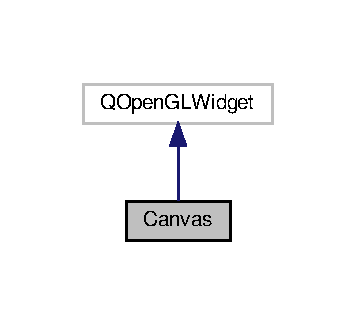
\includegraphics[width=171pt]{class_canvas__inherit__graph}
\end{center}
\end{figure}


Collaboration diagram for Canvas\+:
\nopagebreak
\begin{figure}[H]
\begin{center}
\leavevmode
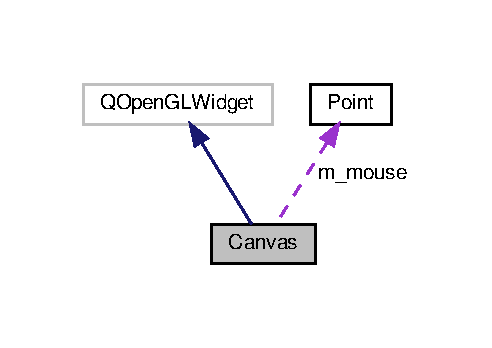
\includegraphics[width=236pt]{class_canvas__coll__graph}
\end{center}
\end{figure}
\subsection*{Public Member Functions}
\begin{DoxyCompactItemize}
\item 
\hyperlink{class_canvas_a8e5bf913d99dcf0511aaa5fd8c294cde}{Canvas} (Q\+Widget $\ast$parent)
\begin{DoxyCompactList}\small\item\em \hyperlink{class_canvas}{Canvas} Constructor. \end{DoxyCompactList}\item 
void \hyperlink{class_canvas_a68622ac24f847a47270c4e6f566eec3c}{initialize\+GL} ()
\begin{DoxyCompactList}\small\item\em initialize\+GL Open\+GL initialization method \end{DoxyCompactList}\item 
void \hyperlink{class_canvas_a4e9439400dd404eda24cf42ca5ca9972}{paint\+GL} ()
\begin{DoxyCompactList}\small\item\em paint\+GL method called on Open\+GL window refresh \end{DoxyCompactList}\item 
\hyperlink{class_point}{Point} \hyperlink{class_canvas_a5c78c7a84c0f9d5540caeab66b677299}{mouse} () const
\begin{DoxyCompactList}\small\item\em mouse getter method for mouse coordinates \end{DoxyCompactList}\item 
void \hyperlink{class_canvas_a104679999425d8ffdc27454b71e5e1e3}{set\+Mouse} (const \hyperlink{class_point}{Point} \&\hyperlink{class_canvas_a5c78c7a84c0f9d5540caeab66b677299}{mouse})
\begin{DoxyCompactList}\small\item\em set\+Mouse setter method for mouse coordinates \end{DoxyCompactList}\item 
int \hyperlink{class_canvas_a63f657b762d08168f52630bc49efbf71}{static\+State} () const
\begin{DoxyCompactList}\small\item\em static\+State getter method for state of static primitive \end{DoxyCompactList}\item 
void \hyperlink{class_canvas_a6c42c7c65e5eae64c4fa1839146f0440}{set\+Static\+State} (int \hyperlink{class_canvas_a63f657b762d08168f52630bc49efbf71}{static\+State})
\begin{DoxyCompactList}\small\item\em set\+Static\+State setter method for state of static primitive \end{DoxyCompactList}\item 
int \hyperlink{class_canvas_a8097ff7e44fb5fecf0dd0997e13e4c32}{moving\+State} () const
\begin{DoxyCompactList}\small\item\em moving\+State getter method for state of moving primitive \end{DoxyCompactList}\item 
void \hyperlink{class_canvas_a3ec03d6ae21250fcc0b0a3164f701933}{set\+Moving\+State} (int \hyperlink{class_canvas_a8097ff7e44fb5fecf0dd0997e13e4c32}{moving\+State})
\begin{DoxyCompactList}\small\item\em set\+Moving\+State setter method for state of moving primitive \end{DoxyCompactList}\end{DoxyCompactItemize}
\subsection*{Static Public Attributes}
\begin{DoxyCompactItemize}
\item 
static const int \hyperlink{class_canvas_a3d5a1c71903689cf817cd92ae7a2ebc9}{T\+OP} = 100
\begin{DoxyCompactList}\small\item\em T\+OP Top of the canvas. \end{DoxyCompactList}\item 
static const int \hyperlink{class_canvas_a0630c650c5daea2db5a01ce6c0954457}{B\+O\+T\+T\+OM} = -\/100
\begin{DoxyCompactList}\small\item\em B\+O\+T\+T\+OM Bottom of the canvas. \end{DoxyCompactList}\item 
static const int \hyperlink{class_canvas_a7da74603fc4232dfe00be701878d048b}{L\+E\+FT} = -\/100
\begin{DoxyCompactList}\small\item\em L\+E\+FT Left of the canvas. \end{DoxyCompactList}\item 
static const int \hyperlink{class_canvas_ab618bb921e1c0ee7c394fe3a83b17271}{R\+I\+G\+HT} = 100
\begin{DoxyCompactList}\small\item\em R\+I\+G\+HT Right on the canvas. \end{DoxyCompactList}\item 
static const int \hyperlink{class_canvas_a04b852dd0b2561a20a5e0e9f67a95b64}{P\+O\+I\+NT} = 0
\begin{DoxyCompactList}\small\item\em P\+O\+I\+NT set primitive to point. \end{DoxyCompactList}\item 
static const int \hyperlink{class_canvas_a28b792bd16aaf737eab6d697a211183a}{L\+I\+NE} = 1
\begin{DoxyCompactList}\small\item\em L\+I\+NE set primitive to line segment. \end{DoxyCompactList}\item 
static const int \hyperlink{class_canvas_a6d5c5da10948c78b6481ac831f32106f}{C\+I\+R\+C\+LE} = 2
\begin{DoxyCompactList}\small\item\em C\+I\+R\+C\+LE set primitive to circle. \end{DoxyCompactList}\item 
static const int \hyperlink{class_canvas_a7d54031701bd0ddbe165a6d4350ab9d6}{T\+R\+I\+A\+N\+G\+LE} = 3
\begin{DoxyCompactList}\small\item\em T\+R\+I\+A\+N\+G\+LE set primitive to triangle. \end{DoxyCompactList}\item 
static const int \hyperlink{class_canvas_a2d0245c75d7fc30adb8abd303844c10f}{S\+Q\+U\+A\+RE} = 4
\begin{DoxyCompactList}\small\item\em S\+Q\+U\+A\+RE set primitive to square. \end{DoxyCompactList}\end{DoxyCompactItemize}
\subsection*{Private Member Functions}
\begin{DoxyCompactItemize}
\item 
void \hyperlink{class_canvas_a0b546aa7d55d00f82b4db59ab4ab9cee}{prepare\+Draw} ()
\begin{DoxyCompactList}\small\item\em prepare\+Draw method to intialze canvas options per draw sequence \end{DoxyCompactList}\item 
void \hyperlink{class_canvas_ad9205f4414565884776edc5f421954a8}{draw\+Gridlines} (int granularity, float shade)
\begin{DoxyCompactList}\small\item\em draw\+Gridlines Used to draw grid lines across full canvas \end{DoxyCompactList}\item 
void \hyperlink{class_canvas_a9fb4b83a1067ddc2aa04676f51dc5a47}{mouse\+Move\+Event} (Q\+Mouse\+Event $\ast$event)
\begin{DoxyCompactList}\small\item\em mouse\+Move\+Event qt method to catch mouse movement events \end{DoxyCompactList}\item 
float \hyperlink{class_canvas_afddf8ae4dcfb9557ae557b9f998f5d5a}{convertedX} (float windowX)
\begin{DoxyCompactList}\small\item\em convertedX converts display x coordinate to canvas x coordinate \end{DoxyCompactList}\item 
float \hyperlink{class_canvas_a12cbc7e3a2cb3bbb6278052d49a90313}{convertedY} (float windowY)
\begin{DoxyCompactList}\small\item\em convertedY converts display y coordinate to canvas y coordinate \end{DoxyCompactList}\item 
void \hyperlink{class_canvas_a78ce810ea0004c4f3fa9ee9d92996875}{draw\+Square} (\hyperlink{class_a_a_b_b}{A\+A\+BB} sq, Q\+Color color)
\begin{DoxyCompactList}\small\item\em draw\+Square draw a square on the canvas \end{DoxyCompactList}\item 
void \hyperlink{class_canvas_ad7cf8e6e93765586808ac744d888dbdc}{draw\+Point} (\hyperlink{class_point}{Point} p, Q\+Color color)
\begin{DoxyCompactList}\small\item\em draw\+Point draw a point on the canvas \end{DoxyCompactList}\item 
void \hyperlink{class_canvas_ae3ad5d92c9a2868b94a6570914b05366}{draw\+Line} (\hyperlink{class_line_segment}{Line\+Segment} line, Q\+Color color)
\begin{DoxyCompactList}\small\item\em draw\+Line draw a line on the canvas \end{DoxyCompactList}\item 
void \hyperlink{class_canvas_ab1413076d90539aea7ac3a06b065afe2}{draw\+Circle} (\hyperlink{class_circle}{Circle} circle, Q\+Color color)
\begin{DoxyCompactList}\small\item\em draw\+Circle draw a circle on the canvas \end{DoxyCompactList}\item 
void \hyperlink{class_canvas_a74dd9cf1e8f3b48e2df2b34886770ac6}{draw\+Triangle} (\hyperlink{class_triangle}{Triangle} t, Q\+Color color)
\begin{DoxyCompactList}\small\item\em draw\+Triangle draw a triangle on the canvas \end{DoxyCompactList}\item 
void \hyperlink{class_canvas_a33b608940212192e7e0ff86c2301c2fe}{point\+Point\+Test} (\hyperlink{class_point}{Point} mv, \hyperlink{class_point}{Point} st)
\begin{DoxyCompactList}\small\item\em point\+Point\+Test test to call when two points need to be tested \end{DoxyCompactList}\item 
void \hyperlink{class_canvas_ad5681f0cada49f0453158155b42c2fb7}{point\+Line\+Test} (\hyperlink{class_point}{Point} p, \hyperlink{class_line_segment}{Line\+Segment} ls)
\begin{DoxyCompactList}\small\item\em point\+Line\+Test test to call when point and line segment need to be tested \end{DoxyCompactList}\item 
void \hyperlink{class_canvas_a407d5fea40a48519ab368d39739943c4}{point\+Circle\+Test} (\hyperlink{class_point}{Point} p, \hyperlink{class_circle}{Circle} cir)
\begin{DoxyCompactList}\small\item\em point\+Circle\+Test test to call when point and cirlce need to be tested \end{DoxyCompactList}\item 
void \hyperlink{class_canvas_a8c35a24d67af6d8a76be14321c08b7cb}{point\+Triangle\+Test} (\hyperlink{class_point}{Point} p, \hyperlink{class_triangle}{Triangle} t)
\begin{DoxyCompactList}\small\item\em point\+Triangle\+Test test to call when point and triangle need to be tested \end{DoxyCompactList}\item 
void \hyperlink{class_canvas_ac9278bae8055ec5b0f047393d2f140b2}{point\+Square\+Test} (\hyperlink{class_point}{Point} p, \hyperlink{class_a_a_b_b}{A\+A\+BB} b)
\begin{DoxyCompactList}\small\item\em point\+Square\+Test test to call when point and square need to be tested \end{DoxyCompactList}\item 
void \hyperlink{class_canvas_ac3e9882133dc6c55f8ff3bb119a8ed84}{line\+Line\+Test} (\hyperlink{class_line_segment}{Line\+Segment} a, \hyperlink{class_line_segment}{Line\+Segment} b)
\begin{DoxyCompactList}\small\item\em line\+Line\+Test test to call when two linesegment need to be tested \end{DoxyCompactList}\item 
void \hyperlink{class_canvas_a1c17d6af0a8770dc2022986cd27e4de4}{line\+Circle\+Test} (\hyperlink{class_line_segment}{Line\+Segment} ls, \hyperlink{class_circle}{Circle} cir)
\begin{DoxyCompactList}\small\item\em line\+Circle\+Test test to call when linesegment and circle need to be tested \end{DoxyCompactList}\item 
void \hyperlink{class_canvas_a39de2e31ab9a27b918fc4f7e78ee2030}{line\+Triangle\+Test} (\hyperlink{class_line_segment}{Line\+Segment} ls, \hyperlink{class_triangle}{Triangle} t)
\begin{DoxyCompactList}\small\item\em line\+Triangle\+Test test to call when linesegment and triangle need to be tested \end{DoxyCompactList}\item 
void \hyperlink{class_canvas_a2eaf680341aebbab7792cd136c2be950}{line\+Square\+Test} (\hyperlink{class_line_segment}{Line\+Segment} ls, \hyperlink{class_a_a_b_b}{A\+A\+BB} sq)
\begin{DoxyCompactList}\small\item\em line\+Square\+Test test to call when linesegment and triangle need to be tested \end{DoxyCompactList}\item 
void \hyperlink{class_canvas_afefa6855ba41959bd86059c3a243b837}{circle\+Circle\+Test} (\hyperlink{class_circle}{Circle} a, \hyperlink{class_circle}{Circle} b)
\begin{DoxyCompactList}\small\item\em circle\+Circle\+Test test to call when two circles need to be tested \end{DoxyCompactList}\item 
void \hyperlink{class_canvas_a528559214b858f9f9cd0a57ca95fb630}{circle\+Triangle\+Test} (\hyperlink{class_circle}{Circle} cir, \hyperlink{class_triangle}{Triangle} t)
\begin{DoxyCompactList}\small\item\em circle\+Triangle\+Test test to call when circle and triangle need to be tested \end{DoxyCompactList}\item 
void \hyperlink{class_canvas_ad9d725683b22b2dc7a5974fed63c16bb}{circle\+Square\+Test} (\hyperlink{class_circle}{Circle} cir, \hyperlink{class_a_a_b_b}{A\+A\+BB} sq)
\begin{DoxyCompactList}\small\item\em circle\+Square\+Test test to call when a circle and square need to be tested \end{DoxyCompactList}\item 
void \hyperlink{class_canvas_a03c673b6f4e09524d322a8c00c5a49f2}{triangle\+Triangle\+Test} (\hyperlink{class_triangle}{Triangle} a, \hyperlink{class_triangle}{Triangle} b)
\begin{DoxyCompactList}\small\item\em triangle\+Triangle\+Test test to call when two triangles need to be tested \end{DoxyCompactList}\item 
void \hyperlink{class_canvas_a8b0b8a040b3e5628a2ec2a89a3025eae}{triangle\+Square\+Test} (\hyperlink{class_triangle}{Triangle} t, \hyperlink{class_a_a_b_b}{A\+A\+BB} sq)
\begin{DoxyCompactList}\small\item\em triangle\+Square\+Test test to call when triangle and circle need to be tested \end{DoxyCompactList}\item 
void \hyperlink{class_canvas_a56718ad140b37cabc6b34157903886ee}{square\+Square\+Test} (\hyperlink{class_a_a_b_b}{A\+A\+BB} a, \hyperlink{class_a_a_b_b}{A\+A\+BB} b)
\begin{DoxyCompactList}\small\item\em square\+Square\+Test test to call when two squares need to be tested \end{DoxyCompactList}\end{DoxyCompactItemize}
\subsection*{Private Attributes}
\begin{DoxyCompactItemize}
\item 
\hyperlink{class_point}{Point} \hyperlink{class_canvas_a37d2fd203dc21501aee37001e49789b1}{m\+\_\+mouse}
\item 
int \hyperlink{class_canvas_adb29cf13087e13c9d4a1ef04bc53b931}{m\+\_\+static\+State} = 4
\item 
int \hyperlink{class_canvas_a0d0f98258b42bd7b40f175baf3f1220a}{m\+\_\+moving\+State} = 0
\end{DoxyCompactItemize}


\subsection{Detailed Description}
Intersection Tester -\/ v1.\+0.\+0 Original Author\+: Liam Mc\+Nabb Proceeding Author(s)\+: N/A Copyright (c) 2019 Permission is hereby granted, free of charge, to any person obtaining a copy of this software and associated documentation files (Intersection\+Tester), to deal in the Software without restriction, including without limitation the rights to use, copy, modify, merge, publish, distribute, sublicense, and/or sell copies of the Software, and to permit persons to whom the Software is furnished to do so, subject to the following conditions\+: The above copyright notice and this permission notice shall be included in all copies or substantial portions of the Software. T\+HE S\+O\+F\+T\+W\+A\+RE IS P\+R\+O\+V\+I\+D\+ED \char`\"{}\+A\+S I\+S\char`\"{}, W\+I\+T\+H\+O\+UT W\+A\+R\+R\+A\+N\+TY OF A\+NY K\+I\+ND, E\+X\+P\+R\+E\+SS OR I\+M\+P\+L\+I\+ED, I\+N\+C\+L\+U\+D\+I\+NG B\+UT N\+OT L\+I\+M\+I\+T\+ED TO T\+HE W\+A\+R\+R\+A\+N\+T\+I\+ES OF M\+E\+R\+C\+H\+A\+N\+T\+A\+B\+I\+L\+I\+TY, F\+I\+T\+N\+E\+SS F\+OR A P\+A\+R\+T\+I\+C\+U\+L\+AR P\+U\+R\+P\+O\+SE A\+ND N\+O\+N\+I\+N\+F\+R\+I\+N\+G\+E\+M\+E\+NT. IN NO E\+V\+E\+NT S\+H\+A\+LL T\+HE A\+U\+T\+H\+O\+RS OR C\+O\+P\+Y\+R\+I\+G\+HT H\+O\+L\+D\+E\+RS BE L\+I\+A\+B\+LE F\+OR A\+NY C\+L\+A\+IM, D\+A\+M\+A\+G\+ES OR O\+T\+H\+ER L\+I\+A\+B\+I\+L\+I\+TY, W\+H\+E\+T\+H\+ER IN AN A\+C\+T\+I\+ON OF C\+O\+N\+T\+R\+A\+CT, T\+O\+RT OR O\+T\+H\+E\+R\+W\+I\+SE, A\+R\+I\+S\+I\+NG F\+R\+OM, O\+UT OF OR IN C\+O\+N\+N\+E\+C\+T\+I\+ON W\+I\+TH T\+HE S\+O\+F\+T\+W\+A\+RE OR T\+HE U\+SE OR O\+T\+H\+ER D\+E\+A\+L\+I\+N\+GS IN T\+HE S\+O\+F\+T\+W\+A\+RE. 

Definition at line 35 of file canvas.\+h.



\subsection{Constructor \& Destructor Documentation}
\mbox{\Hypertarget{class_canvas_a8e5bf913d99dcf0511aaa5fd8c294cde}\label{class_canvas_a8e5bf913d99dcf0511aaa5fd8c294cde}} 
\index{Canvas@{Canvas}!Canvas@{Canvas}}
\index{Canvas@{Canvas}!Canvas@{Canvas}}
\subsubsection{\texorpdfstring{Canvas()}{Canvas()}}
{\footnotesize\ttfamily Canvas\+::\+Canvas (\begin{DoxyParamCaption}\item[{Q\+Widget $\ast$}]{parent }\end{DoxyParamCaption})}



\hyperlink{class_canvas}{Canvas} Constructor. 


\begin{DoxyParams}{Parameters}
{\em parent} & parent window \\
\hline
\end{DoxyParams}


Definition at line 3 of file canvas.\+cpp.


\begin{DoxyCode}
3                                 : QOpenGLWidget( parent )
4 \{
5     \hyperlink{class_intersect_tester_ac837c3469e328c8bb47d08742c304c9a}{IntersectTester::setTolerance}( 1.0f );
6 \}
\end{DoxyCode}


\subsection{Member Function Documentation}
\mbox{\Hypertarget{class_canvas_afefa6855ba41959bd86059c3a243b837}\label{class_canvas_afefa6855ba41959bd86059c3a243b837}} 
\index{Canvas@{Canvas}!circle\+Circle\+Test@{circle\+Circle\+Test}}
\index{circle\+Circle\+Test@{circle\+Circle\+Test}!Canvas@{Canvas}}
\subsubsection{\texorpdfstring{circle\+Circle\+Test()}{circleCircleTest()}}
{\footnotesize\ttfamily void Canvas\+::circle\+Circle\+Test (\begin{DoxyParamCaption}\item[{\hyperlink{class_circle}{Circle}}]{a,  }\item[{\hyperlink{class_circle}{Circle}}]{b }\end{DoxyParamCaption})\hspace{0.3cm}{\ttfamily [private]}}



circle\+Circle\+Test test to call when two circles need to be tested 


\begin{DoxyParams}{Parameters}
{\em a} & circle 1 \\
\hline
{\em b} & circle 2 \\
\hline
\end{DoxyParams}


Definition at line 299 of file canvas.\+cpp.


\begin{DoxyCode}
300 \{
301     QColor c = Qt::black;
302     \textcolor{keywordflow}{if}(\hyperlink{class_intersect_tester_a7710e17ff7d2e229059f23b9429213f5}{IntersectTester::isIntersecting}(a, b))
303         c = Qt::green;
304 
305     \hyperlink{class_canvas_ab1413076d90539aea7ac3a06b065afe2}{drawCircle}(a,c);
306     \hyperlink{class_canvas_ab1413076d90539aea7ac3a06b065afe2}{drawCircle}(b,c);
307 \}
\end{DoxyCode}
\mbox{\Hypertarget{class_canvas_ad9d725683b22b2dc7a5974fed63c16bb}\label{class_canvas_ad9d725683b22b2dc7a5974fed63c16bb}} 
\index{Canvas@{Canvas}!circle\+Square\+Test@{circle\+Square\+Test}}
\index{circle\+Square\+Test@{circle\+Square\+Test}!Canvas@{Canvas}}
\subsubsection{\texorpdfstring{circle\+Square\+Test()}{circleSquareTest()}}
{\footnotesize\ttfamily void Canvas\+::circle\+Square\+Test (\begin{DoxyParamCaption}\item[{\hyperlink{class_circle}{Circle}}]{cir,  }\item[{\hyperlink{class_a_a_b_b}{A\+A\+BB}}]{sq }\end{DoxyParamCaption})\hspace{0.3cm}{\ttfamily [private]}}



circle\+Square\+Test test to call when a circle and square need to be tested 


\begin{DoxyParams}{Parameters}
{\em cir} & circle \\
\hline
{\em sq} & square \\
\hline
\end{DoxyParams}


Definition at line 319 of file canvas.\+cpp.


\begin{DoxyCode}
320 \{
321     \hyperlink{class_point}{Point} A(sq.\hyperlink{class_a_a_b_b_aaf1ec35e5c0258cd57e65429f93c14a2}{minimums}[\hyperlink{class_a_a_b_b_aac753e0248d039329b25b38d0ed9cd4f}{AABB::XDIM}], sq.\hyperlink{class_a_a_b_b_aaf1ec35e5c0258cd57e65429f93c14a2}{minimums}[
      \hyperlink{class_a_a_b_b_a5192e3bdf0789cdc9e5f643b401e5b10}{AABB::YDIM}]);
322     \hyperlink{class_point}{Point} B(sq.\hyperlink{class_a_a_b_b_aaf1ec35e5c0258cd57e65429f93c14a2}{minimums}[\hyperlink{class_a_a_b_b_aac753e0248d039329b25b38d0ed9cd4f}{AABB::XDIM}], sq.\hyperlink{class_a_a_b_b_a1289c3a2e5c7a98f90d5bcdb8251a06f}{maximums}[
      \hyperlink{class_a_a_b_b_a5192e3bdf0789cdc9e5f643b401e5b10}{AABB::YDIM}]);
323     \hyperlink{class_point}{Point} C(sq.\hyperlink{class_a_a_b_b_a1289c3a2e5c7a98f90d5bcdb8251a06f}{maximums}[\hyperlink{class_a_a_b_b_aac753e0248d039329b25b38d0ed9cd4f}{AABB::XDIM}], sq.\hyperlink{class_a_a_b_b_a1289c3a2e5c7a98f90d5bcdb8251a06f}{maximums}[
      \hyperlink{class_a_a_b_b_a5192e3bdf0789cdc9e5f643b401e5b10}{AABB::YDIM}]);
324     \hyperlink{class_point}{Point} D(sq.\hyperlink{class_a_a_b_b_a1289c3a2e5c7a98f90d5bcdb8251a06f}{maximums}[\hyperlink{class_a_a_b_b_aac753e0248d039329b25b38d0ed9cd4f}{AABB::XDIM}], sq.\hyperlink{class_a_a_b_b_aaf1ec35e5c0258cd57e65429f93c14a2}{minimums}[
      \hyperlink{class_a_a_b_b_a5192e3bdf0789cdc9e5f643b401e5b10}{AABB::YDIM}]);
325 
326     QColor c = Qt::black;
327     \textcolor{keywordflow}{if}(\hyperlink{class_intersect_tester_a7710e17ff7d2e229059f23b9429213f5}{IntersectTester::isIntersecting}(cir, sq))
328         c = Qt::green;
329 
330     \hyperlink{class_canvas_ad7cf8e6e93765586808ac744d888dbdc}{drawPoint}(\hyperlink{class_intersect_tester_a6bb20d4839643fbfd53a5d4506448a92}{IntersectTester::closestPoint}( 
      \hyperlink{class_line_segment}{LineSegment}(A,B), cir.\hyperlink{class_circle_a9818ca0bbac64ff447945a8e51ff9319}{getCenter}() ),Qt::black);
331     \hyperlink{class_canvas_ad7cf8e6e93765586808ac744d888dbdc}{drawPoint}(\hyperlink{class_intersect_tester_a6bb20d4839643fbfd53a5d4506448a92}{IntersectTester::closestPoint}( 
      \hyperlink{class_line_segment}{LineSegment}(B,C), cir.\hyperlink{class_circle_a9818ca0bbac64ff447945a8e51ff9319}{getCenter}() ),Qt::black);
332     \hyperlink{class_canvas_ad7cf8e6e93765586808ac744d888dbdc}{drawPoint}(\hyperlink{class_intersect_tester_a6bb20d4839643fbfd53a5d4506448a92}{IntersectTester::closestPoint}( 
      \hyperlink{class_line_segment}{LineSegment}(D,C), cir.\hyperlink{class_circle_a9818ca0bbac64ff447945a8e51ff9319}{getCenter}() ),Qt::black);
333     \hyperlink{class_canvas_ad7cf8e6e93765586808ac744d888dbdc}{drawPoint}(\hyperlink{class_intersect_tester_a6bb20d4839643fbfd53a5d4506448a92}{IntersectTester::closestPoint}( 
      \hyperlink{class_line_segment}{LineSegment}(A,D), cir.\hyperlink{class_circle_a9818ca0bbac64ff447945a8e51ff9319}{getCenter}() ),Qt::black);
334     \hyperlink{class_canvas_ab1413076d90539aea7ac3a06b065afe2}{drawCircle}(cir,c);
335     \hyperlink{class_canvas_a78ce810ea0004c4f3fa9ee9d92996875}{drawSquare}(sq,c);
336 \}
\end{DoxyCode}
\mbox{\Hypertarget{class_canvas_a528559214b858f9f9cd0a57ca95fb630}\label{class_canvas_a528559214b858f9f9cd0a57ca95fb630}} 
\index{Canvas@{Canvas}!circle\+Triangle\+Test@{circle\+Triangle\+Test}}
\index{circle\+Triangle\+Test@{circle\+Triangle\+Test}!Canvas@{Canvas}}
\subsubsection{\texorpdfstring{circle\+Triangle\+Test()}{circleTriangleTest()}}
{\footnotesize\ttfamily void Canvas\+::circle\+Triangle\+Test (\begin{DoxyParamCaption}\item[{\hyperlink{class_circle}{Circle}}]{cir,  }\item[{\hyperlink{class_triangle}{Triangle}}]{t }\end{DoxyParamCaption})\hspace{0.3cm}{\ttfamily [private]}}



circle\+Triangle\+Test test to call when circle and triangle need to be tested 


\begin{DoxyParams}{Parameters}
{\em cir} & circle \\
\hline
{\em t} & triangle \\
\hline
\end{DoxyParams}


Definition at line 309 of file canvas.\+cpp.


\begin{DoxyCode}
310 \{
311     QColor c = Qt::black;
312     \textcolor{keywordflow}{if}(\hyperlink{class_intersect_tester_a7710e17ff7d2e229059f23b9429213f5}{IntersectTester::isIntersecting}(cir, t))
313         c = Qt::green;
314 
315     \hyperlink{class_canvas_ab1413076d90539aea7ac3a06b065afe2}{drawCircle}(cir,c);
316     \hyperlink{class_canvas_a74dd9cf1e8f3b48e2df2b34886770ac6}{drawTriangle}(t,c);
317 \}
\end{DoxyCode}
\mbox{\Hypertarget{class_canvas_afddf8ae4dcfb9557ae557b9f998f5d5a}\label{class_canvas_afddf8ae4dcfb9557ae557b9f998f5d5a}} 
\index{Canvas@{Canvas}!convertedX@{convertedX}}
\index{convertedX@{convertedX}!Canvas@{Canvas}}
\subsubsection{\texorpdfstring{converted\+X()}{convertedX()}}
{\footnotesize\ttfamily float Canvas\+::convertedX (\begin{DoxyParamCaption}\item[{float}]{windowX }\end{DoxyParamCaption})\hspace{0.3cm}{\ttfamily [private]}}



convertedX converts display x coordinate to canvas x coordinate 


\begin{DoxyParams}{Parameters}
{\em windowX} & display x coordinate \\
\hline
\end{DoxyParams}
\begin{DoxyReturn}{Returns}
canvas x coordinate 
\end{DoxyReturn}


Definition at line 496 of file canvas.\+cpp.


\begin{DoxyCode}
497 \{
498     \textcolor{keywordtype}{float} newX;
499     newX = \hyperlink{class_canvas_a7da74603fc4232dfe00be701878d048b}{LEFT} +
500             ( ( windowX / this->width() ) *
501               ( \hyperlink{class_canvas_ab618bb921e1c0ee7c394fe3a83b17271}{RIGHT} - \hyperlink{class_canvas_a7da74603fc4232dfe00be701878d048b}{LEFT} ) );
502     \textcolor{keywordflow}{return} newX;
503 \}
\end{DoxyCode}
\mbox{\Hypertarget{class_canvas_a12cbc7e3a2cb3bbb6278052d49a90313}\label{class_canvas_a12cbc7e3a2cb3bbb6278052d49a90313}} 
\index{Canvas@{Canvas}!convertedY@{convertedY}}
\index{convertedY@{convertedY}!Canvas@{Canvas}}
\subsubsection{\texorpdfstring{converted\+Y()}{convertedY()}}
{\footnotesize\ttfamily float Canvas\+::convertedY (\begin{DoxyParamCaption}\item[{float}]{windowY }\end{DoxyParamCaption})\hspace{0.3cm}{\ttfamily [private]}}



convertedY converts display y coordinate to canvas y coordinate 


\begin{DoxyParams}{Parameters}
{\em windowY} & display y coordinate \\
\hline
\end{DoxyParams}
\begin{DoxyReturn}{Returns}
canvas y coordinate 
\end{DoxyReturn}


Definition at line 505 of file canvas.\+cpp.


\begin{DoxyCode}
506 \{
507     \textcolor{keywordtype}{float} newY,reverseY;
508     reverseY = -( windowY - 1 - this->height() );
509 
510     newY = \hyperlink{class_canvas_a0630c650c5daea2db5a01ce6c0954457}{BOTTOM} +
511             ( ( reverseY / this->height() ) *
512               ( \hyperlink{class_canvas_a3d5a1c71903689cf817cd92ae7a2ebc9}{TOP} - \hyperlink{class_canvas_a0630c650c5daea2db5a01ce6c0954457}{BOTTOM} ) ) ;
513     \textcolor{keywordflow}{return} newY;
514 \}
\end{DoxyCode}
\mbox{\Hypertarget{class_canvas_ab1413076d90539aea7ac3a06b065afe2}\label{class_canvas_ab1413076d90539aea7ac3a06b065afe2}} 
\index{Canvas@{Canvas}!draw\+Circle@{draw\+Circle}}
\index{draw\+Circle@{draw\+Circle}!Canvas@{Canvas}}
\subsubsection{\texorpdfstring{draw\+Circle()}{drawCircle()}}
{\footnotesize\ttfamily void Canvas\+::draw\+Circle (\begin{DoxyParamCaption}\item[{\hyperlink{class_circle}{Circle}}]{circle,  }\item[{Q\+Color}]{color }\end{DoxyParamCaption})\hspace{0.3cm}{\ttfamily [private]}}



draw\+Circle draw a circle on the canvas 


\begin{DoxyParams}{Parameters}
{\em circle} & circle to draw \\
\hline
{\em color} & the color of the circle \\
\hline
\end{DoxyParams}


Definition at line 385 of file canvas.\+cpp.


\begin{DoxyCode}
386 \{
387     glColor3f(color.redF(),color.greenF(),color.blueF());
388     glBegin(GL\_LINE\_LOOP);
389     \textcolor{keywordflow}{for} ( \textcolor{keywordtype}{float} angle = 0; angle <= (2*M\_PI); angle += 0.01 )
390     \{
391         \textcolor{keywordtype}{float} x = circle.\hyperlink{class_circle_a9818ca0bbac64ff447945a8e51ff9319}{getCenter}().\hyperlink{class_point_a29c44ec7c7279e02629645a06cdaf7d5}{getX}() + sin( angle ) *
392                     circle.\hyperlink{class_circle_a95b7dc25d2e9b1e40a189cd83386a12e}{getRadius}();
393 
394         \textcolor{keywordtype}{float} y = circle.\hyperlink{class_circle_a9818ca0bbac64ff447945a8e51ff9319}{getCenter}().\hyperlink{class_point_a2371ffadbe245d12a8f556d0a976521b}{getY}() + cos( angle ) *
395                     circle.\hyperlink{class_circle_a95b7dc25d2e9b1e40a189cd83386a12e}{getRadius}();
396 
397         glVertex2f( x, y );
398     \}
399     glEnd();
400 
401     glColor4f(color.redF(),color.greenF(),color.blueF(), 0.2f);
402     glBegin( GL\_TRIANGLE\_FAN );
403     glVertex2f( circle.\hyperlink{class_circle_a9818ca0bbac64ff447945a8e51ff9319}{getCenter}().\hyperlink{class_point_a29c44ec7c7279e02629645a06cdaf7d5}{getX}(), circle.\hyperlink{class_circle_a9818ca0bbac64ff447945a8e51ff9319}{getCenter}().
      \hyperlink{class_point_a2371ffadbe245d12a8f556d0a976521b}{getY}() );
404     \textcolor{keywordflow}{for} ( \textcolor{keywordtype}{float} angle = 0; angle <= (2*M\_PI); angle += 0.01 )
405     \{
406         \textcolor{keywordtype}{float} x = circle.\hyperlink{class_circle_a9818ca0bbac64ff447945a8e51ff9319}{getCenter}().\hyperlink{class_point_a29c44ec7c7279e02629645a06cdaf7d5}{getX}() + sin( angle ) *
407                     circle.\hyperlink{class_circle_a95b7dc25d2e9b1e40a189cd83386a12e}{getRadius}();
408 
409         \textcolor{keywordtype}{float} y = circle.\hyperlink{class_circle_a9818ca0bbac64ff447945a8e51ff9319}{getCenter}().\hyperlink{class_point_a2371ffadbe245d12a8f556d0a976521b}{getY}() + cos( angle ) *
410                     circle.\hyperlink{class_circle_a95b7dc25d2e9b1e40a189cd83386a12e}{getRadius}();
411 
412         glVertex2f( x, y );
413     \}
414     \textcolor{keywordtype}{float} x = circle.\hyperlink{class_circle_a9818ca0bbac64ff447945a8e51ff9319}{getCenter}().\hyperlink{class_point_a29c44ec7c7279e02629645a06cdaf7d5}{getX}() + sin( 0 ) *
415                 circle.\hyperlink{class_circle_a95b7dc25d2e9b1e40a189cd83386a12e}{getRadius}();
416 
417     \textcolor{keywordtype}{float} y = circle.\hyperlink{class_circle_a9818ca0bbac64ff447945a8e51ff9319}{getCenter}().\hyperlink{class_point_a2371ffadbe245d12a8f556d0a976521b}{getY}() + cos( 0 ) *
418                 circle.\hyperlink{class_circle_a95b7dc25d2e9b1e40a189cd83386a12e}{getRadius}() ;
419 
420     glVertex2f( x, y );
421     glEnd();
422 \}
\end{DoxyCode}
\mbox{\Hypertarget{class_canvas_ad9205f4414565884776edc5f421954a8}\label{class_canvas_ad9205f4414565884776edc5f421954a8}} 
\index{Canvas@{Canvas}!draw\+Gridlines@{draw\+Gridlines}}
\index{draw\+Gridlines@{draw\+Gridlines}!Canvas@{Canvas}}
\subsubsection{\texorpdfstring{draw\+Gridlines()}{drawGridlines()}}
{\footnotesize\ttfamily void Canvas\+::draw\+Gridlines (\begin{DoxyParamCaption}\item[{int}]{granularity,  }\item[{float}]{shade }\end{DoxyParamCaption})\hspace{0.3cm}{\ttfamily [private]}}



draw\+Gridlines Used to draw grid lines across full canvas 


\begin{DoxyParams}{Parameters}
{\em granularity} & how many lifes drawn grid segments per dimension \\
\hline
{\em shade} & the greyscale shade of the grid \\
\hline
\end{DoxyParams}


Definition at line 460 of file canvas.\+cpp.


\begin{DoxyCode}
461 \{
462     \textcolor{keywordtype}{int} gap = ( \hyperlink{class_canvas_a3d5a1c71903689cf817cd92ae7a2ebc9}{TOP} - \hyperlink{class_canvas_a0630c650c5daea2db5a01ce6c0954457}{BOTTOM} ) / granularity;
463     glColor3f(shade,shade,shade);
464     glBegin(GL\_LINES);
465     \textcolor{keywordflow}{for} ( \textcolor{keywordtype}{int} i = 0; i < granularity; ++i )
466     \{
467         \textcolor{keywordtype}{int} x = \hyperlink{class_canvas_a7da74603fc4232dfe00be701878d048b}{LEFT} + (gap*i);
468         glVertex2f(x,\hyperlink{class_canvas_a0630c650c5daea2db5a01ce6c0954457}{BOTTOM});
469         glVertex2f(x,\hyperlink{class_canvas_a3d5a1c71903689cf817cd92ae7a2ebc9}{TOP});
470 
471         \textcolor{keywordtype}{int} y = \hyperlink{class_canvas_a0630c650c5daea2db5a01ce6c0954457}{BOTTOM} + (gap*i);
472         glVertex2f(\hyperlink{class_canvas_a7da74603fc4232dfe00be701878d048b}{LEFT},y);
473         glVertex2f(\hyperlink{class_canvas_ab618bb921e1c0ee7c394fe3a83b17271}{RIGHT},y);
474 
475     \}
476     glEnd();
477 \}
\end{DoxyCode}
\mbox{\Hypertarget{class_canvas_ae3ad5d92c9a2868b94a6570914b05366}\label{class_canvas_ae3ad5d92c9a2868b94a6570914b05366}} 
\index{Canvas@{Canvas}!draw\+Line@{draw\+Line}}
\index{draw\+Line@{draw\+Line}!Canvas@{Canvas}}
\subsubsection{\texorpdfstring{draw\+Line()}{drawLine()}}
{\footnotesize\ttfamily void Canvas\+::draw\+Line (\begin{DoxyParamCaption}\item[{\hyperlink{class_line_segment}{Line\+Segment}}]{line,  }\item[{Q\+Color}]{color }\end{DoxyParamCaption})\hspace{0.3cm}{\ttfamily [private]}}



draw\+Line draw a line on the canvas 


\begin{DoxyParams}{Parameters}
{\em line} & line to draw \\
\hline
{\em color} & the color of the line \\
\hline
\end{DoxyParams}


Definition at line 376 of file canvas.\+cpp.


\begin{DoxyCode}
377 \{
378     glColor3f(color.redF(),color.greenF(),color.blueF());
379     glBegin(GL\_LINES);
380     glVertex2f(line.\hyperlink{class_line_segment_afcff6bd5f6a3073a44f7b21db0be876f}{getStart}().\hyperlink{class_point_a29c44ec7c7279e02629645a06cdaf7d5}{getX}(), line.\hyperlink{class_line_segment_afcff6bd5f6a3073a44f7b21db0be876f}{getStart}().\hyperlink{class_point_a2371ffadbe245d12a8f556d0a976521b}{getY}());
381     glVertex2f(line.\hyperlink{class_line_segment_a7b05f883c369b950e61009edfafbbd0e}{getEnd}().\hyperlink{class_point_a29c44ec7c7279e02629645a06cdaf7d5}{getX}(), line.\hyperlink{class_line_segment_a7b05f883c369b950e61009edfafbbd0e}{getEnd}().\hyperlink{class_point_a2371ffadbe245d12a8f556d0a976521b}{getY}());
382     glEnd();
383 \}
\end{DoxyCode}
\mbox{\Hypertarget{class_canvas_ad7cf8e6e93765586808ac744d888dbdc}\label{class_canvas_ad7cf8e6e93765586808ac744d888dbdc}} 
\index{Canvas@{Canvas}!draw\+Point@{draw\+Point}}
\index{draw\+Point@{draw\+Point}!Canvas@{Canvas}}
\subsubsection{\texorpdfstring{draw\+Point()}{drawPoint()}}
{\footnotesize\ttfamily void Canvas\+::draw\+Point (\begin{DoxyParamCaption}\item[{\hyperlink{class_point}{Point}}]{p,  }\item[{Q\+Color}]{color }\end{DoxyParamCaption})\hspace{0.3cm}{\ttfamily [private]}}



draw\+Point draw a point on the canvas 


\begin{DoxyParams}{Parameters}
{\em p} & point to draw \\
\hline
{\em color} & the color of the point \\
\hline
\end{DoxyParams}


Definition at line 368 of file canvas.\+cpp.


\begin{DoxyCode}
369 \{
370     glColor3f(color.redF(),color.greenF(),color.blueF());
371     glBegin(GL\_POINTS);
372     glVertex2f(p.\hyperlink{class_point_a29c44ec7c7279e02629645a06cdaf7d5}{getX}(),p.\hyperlink{class_point_a2371ffadbe245d12a8f556d0a976521b}{getY}());
373     glEnd();
374 \}
\end{DoxyCode}
\mbox{\Hypertarget{class_canvas_a78ce810ea0004c4f3fa9ee9d92996875}\label{class_canvas_a78ce810ea0004c4f3fa9ee9d92996875}} 
\index{Canvas@{Canvas}!draw\+Square@{draw\+Square}}
\index{draw\+Square@{draw\+Square}!Canvas@{Canvas}}
\subsubsection{\texorpdfstring{draw\+Square()}{drawSquare()}}
{\footnotesize\ttfamily void Canvas\+::draw\+Square (\begin{DoxyParamCaption}\item[{\hyperlink{class_a_a_b_b}{A\+A\+BB}}]{sq,  }\item[{Q\+Color}]{color }\end{DoxyParamCaption})\hspace{0.3cm}{\ttfamily [private]}}



draw\+Square draw a square on the canvas 


\begin{DoxyParams}{Parameters}
{\em sq} & the square to draw \\
\hline
{\em color} & the color of the square \\
\hline
\end{DoxyParams}


Definition at line 441 of file canvas.\+cpp.


\begin{DoxyCode}
442 \{
443     glColor3f(color.redF(),color.greenF(),color.blueF());
444     glBegin(GL\_LINE\_LOOP);
445     glVertex2f(sq.\hyperlink{class_a_a_b_b_aaf1ec35e5c0258cd57e65429f93c14a2}{minimums}[\hyperlink{class_a_a_b_b_aac753e0248d039329b25b38d0ed9cd4f}{AABB::XDIM}],sq.\hyperlink{class_a_a_b_b_aaf1ec35e5c0258cd57e65429f93c14a2}{minimums}[
      \hyperlink{class_a_a_b_b_a5192e3bdf0789cdc9e5f643b401e5b10}{AABB::YDIM}]);
446     glVertex2f(sq.\hyperlink{class_a_a_b_b_aaf1ec35e5c0258cd57e65429f93c14a2}{minimums}[\hyperlink{class_a_a_b_b_aac753e0248d039329b25b38d0ed9cd4f}{AABB::XDIM}],sq.\hyperlink{class_a_a_b_b_a1289c3a2e5c7a98f90d5bcdb8251a06f}{maximums}[
      \hyperlink{class_a_a_b_b_a5192e3bdf0789cdc9e5f643b401e5b10}{AABB::YDIM}]);
447     glVertex2f(sq.\hyperlink{class_a_a_b_b_a1289c3a2e5c7a98f90d5bcdb8251a06f}{maximums}[\hyperlink{class_a_a_b_b_aac753e0248d039329b25b38d0ed9cd4f}{AABB::XDIM}],sq.\hyperlink{class_a_a_b_b_a1289c3a2e5c7a98f90d5bcdb8251a06f}{maximums}[
      \hyperlink{class_a_a_b_b_a5192e3bdf0789cdc9e5f643b401e5b10}{AABB::YDIM}]);
448     glVertex2f(sq.\hyperlink{class_a_a_b_b_a1289c3a2e5c7a98f90d5bcdb8251a06f}{maximums}[\hyperlink{class_a_a_b_b_aac753e0248d039329b25b38d0ed9cd4f}{AABB::XDIM}],sq.\hyperlink{class_a_a_b_b_aaf1ec35e5c0258cd57e65429f93c14a2}{minimums}[
      \hyperlink{class_a_a_b_b_a5192e3bdf0789cdc9e5f643b401e5b10}{AABB::YDIM}]);
449     glEnd();
450 
451     glColor4f(color.redF(),color.greenF(),color.blueF(), 0.2);
452     glBegin(GL\_QUADS);
453     glVertex2f(sq.\hyperlink{class_a_a_b_b_aaf1ec35e5c0258cd57e65429f93c14a2}{minimums}[\hyperlink{class_a_a_b_b_aac753e0248d039329b25b38d0ed9cd4f}{AABB::XDIM}],sq.\hyperlink{class_a_a_b_b_aaf1ec35e5c0258cd57e65429f93c14a2}{minimums}[
      \hyperlink{class_a_a_b_b_a5192e3bdf0789cdc9e5f643b401e5b10}{AABB::YDIM}]);
454     glVertex2f(sq.\hyperlink{class_a_a_b_b_aaf1ec35e5c0258cd57e65429f93c14a2}{minimums}[\hyperlink{class_a_a_b_b_aac753e0248d039329b25b38d0ed9cd4f}{AABB::XDIM}],sq.\hyperlink{class_a_a_b_b_a1289c3a2e5c7a98f90d5bcdb8251a06f}{maximums}[
      \hyperlink{class_a_a_b_b_a5192e3bdf0789cdc9e5f643b401e5b10}{AABB::YDIM}]);
455     glVertex2f(sq.\hyperlink{class_a_a_b_b_a1289c3a2e5c7a98f90d5bcdb8251a06f}{maximums}[\hyperlink{class_a_a_b_b_aac753e0248d039329b25b38d0ed9cd4f}{AABB::XDIM}],sq.\hyperlink{class_a_a_b_b_a1289c3a2e5c7a98f90d5bcdb8251a06f}{maximums}[
      \hyperlink{class_a_a_b_b_a5192e3bdf0789cdc9e5f643b401e5b10}{AABB::YDIM}]);
456     glVertex2f(sq.\hyperlink{class_a_a_b_b_a1289c3a2e5c7a98f90d5bcdb8251a06f}{maximums}[\hyperlink{class_a_a_b_b_aac753e0248d039329b25b38d0ed9cd4f}{AABB::XDIM}],sq.\hyperlink{class_a_a_b_b_aaf1ec35e5c0258cd57e65429f93c14a2}{minimums}[
      \hyperlink{class_a_a_b_b_a5192e3bdf0789cdc9e5f643b401e5b10}{AABB::YDIM}]);
457     glEnd();
458 \}
\end{DoxyCode}
\mbox{\Hypertarget{class_canvas_a74dd9cf1e8f3b48e2df2b34886770ac6}\label{class_canvas_a74dd9cf1e8f3b48e2df2b34886770ac6}} 
\index{Canvas@{Canvas}!draw\+Triangle@{draw\+Triangle}}
\index{draw\+Triangle@{draw\+Triangle}!Canvas@{Canvas}}
\subsubsection{\texorpdfstring{draw\+Triangle()}{drawTriangle()}}
{\footnotesize\ttfamily void Canvas\+::draw\+Triangle (\begin{DoxyParamCaption}\item[{\hyperlink{class_triangle}{Triangle}}]{t,  }\item[{Q\+Color}]{color }\end{DoxyParamCaption})\hspace{0.3cm}{\ttfamily [private]}}



draw\+Triangle draw a triangle on the canvas 


\begin{DoxyParams}{Parameters}
{\em t} & triangle to draw \\
\hline
{\em color} & the color of the triangle \\
\hline
\end{DoxyParams}


Definition at line 424 of file canvas.\+cpp.


\begin{DoxyCode}
425 \{
426     glColor3f(color.redF(),color.greenF(),color.blueF());
427     glBegin(GL\_LINE\_LOOP);
428     glVertex2f(t.\hyperlink{class_triangle_a88a35d0b66c9636a9be88adc88d003aa}{getVertexOne}().\hyperlink{class_point_a29c44ec7c7279e02629645a06cdaf7d5}{getX}(), t.\hyperlink{class_triangle_a88a35d0b66c9636a9be88adc88d003aa}{getVertexOne}().
      \hyperlink{class_point_a2371ffadbe245d12a8f556d0a976521b}{getY}());
429     glVertex2f(t.\hyperlink{class_triangle_ac1ae7463f829bcf377fd926b1ad10cac}{getVertexTwo}().\hyperlink{class_point_a29c44ec7c7279e02629645a06cdaf7d5}{getX}(), t.\hyperlink{class_triangle_ac1ae7463f829bcf377fd926b1ad10cac}{getVertexTwo}().
      \hyperlink{class_point_a2371ffadbe245d12a8f556d0a976521b}{getY}());
430     glVertex2f(t.\hyperlink{class_triangle_aed6ceca804b35da95d3d3c930de41e91}{getVertexThree}().\hyperlink{class_point_a29c44ec7c7279e02629645a06cdaf7d5}{getX}(), t.\hyperlink{class_triangle_aed6ceca804b35da95d3d3c930de41e91}{getVertexThree}().
      \hyperlink{class_point_a2371ffadbe245d12a8f556d0a976521b}{getY}());
431     glEnd();
432 
433     glColor4f(color.redF(),color.greenF(),color.blueF(),0.2);
434     glBegin(GL\_POLYGON);
435     glVertex2f(t.\hyperlink{class_triangle_a88a35d0b66c9636a9be88adc88d003aa}{getVertexOne}().\hyperlink{class_point_a29c44ec7c7279e02629645a06cdaf7d5}{getX}(), t.\hyperlink{class_triangle_a88a35d0b66c9636a9be88adc88d003aa}{getVertexOne}().
      \hyperlink{class_point_a2371ffadbe245d12a8f556d0a976521b}{getY}());
436     glVertex2f(t.\hyperlink{class_triangle_ac1ae7463f829bcf377fd926b1ad10cac}{getVertexTwo}().\hyperlink{class_point_a29c44ec7c7279e02629645a06cdaf7d5}{getX}(), t.\hyperlink{class_triangle_ac1ae7463f829bcf377fd926b1ad10cac}{getVertexTwo}().
      \hyperlink{class_point_a2371ffadbe245d12a8f556d0a976521b}{getY}());
437     glVertex2f(t.\hyperlink{class_triangle_aed6ceca804b35da95d3d3c930de41e91}{getVertexThree}().\hyperlink{class_point_a29c44ec7c7279e02629645a06cdaf7d5}{getX}(), t.\hyperlink{class_triangle_aed6ceca804b35da95d3d3c930de41e91}{getVertexThree}().
      \hyperlink{class_point_a2371ffadbe245d12a8f556d0a976521b}{getY}());
438     glEnd();
439 \}
\end{DoxyCode}
\mbox{\Hypertarget{class_canvas_a68622ac24f847a47270c4e6f566eec3c}\label{class_canvas_a68622ac24f847a47270c4e6f566eec3c}} 
\index{Canvas@{Canvas}!initialize\+GL@{initialize\+GL}}
\index{initialize\+GL@{initialize\+GL}!Canvas@{Canvas}}
\subsubsection{\texorpdfstring{initialize\+G\+L()}{initializeGL()}}
{\footnotesize\ttfamily void Canvas\+::initialize\+GL (\begin{DoxyParamCaption}{ }\end{DoxyParamCaption})}



initialize\+GL Open\+GL initialization method 



Definition at line 8 of file canvas.\+cpp.


\begin{DoxyCode}
9 \{
10 
11     glClear( GL\_COLOR\_BUFFER\_BIT | GL\_DEPTH\_BUFFER\_BIT );
12     glEnable( GL\_BLEND ); \textcolor{comment}{// Required Blending for alpha blending}
13     glEnable( GL\_ALPHA ); \textcolor{comment}{// Lets you add alpha values}
14     \textcolor{comment}{//    glEnable( GL\_LINE\_STIPPLE ); // Enables Dotted Line for use}
15     glBlendFunc( GL\_SRC\_ALPHA, GL\_ONE\_MINUS\_SRC\_ALPHA );
16     glClearColor(1,1,1,1);
17     \textcolor{comment}{//    connect( &timer, SIGNAL( timeout() ), this, SLOT( update() ) );}
18     \textcolor{comment}{//    timer.start( 1000 );}
19     QWidget::setMouseTracking(\textcolor{keyword}{true});
20     \hyperlink{class_canvas_a104679999425d8ffdc27454b71e5e1e3}{setMouse}(\hyperlink{class_point}{Point}(-100,100));
21 
22 \}
\end{DoxyCode}
\mbox{\Hypertarget{class_canvas_a1c17d6af0a8770dc2022986cd27e4de4}\label{class_canvas_a1c17d6af0a8770dc2022986cd27e4de4}} 
\index{Canvas@{Canvas}!line\+Circle\+Test@{line\+Circle\+Test}}
\index{line\+Circle\+Test@{line\+Circle\+Test}!Canvas@{Canvas}}
\subsubsection{\texorpdfstring{line\+Circle\+Test()}{lineCircleTest()}}
{\footnotesize\ttfamily void Canvas\+::line\+Circle\+Test (\begin{DoxyParamCaption}\item[{\hyperlink{class_line_segment}{Line\+Segment}}]{ls,  }\item[{\hyperlink{class_circle}{Circle}}]{cir }\end{DoxyParamCaption})\hspace{0.3cm}{\ttfamily [private]}}



line\+Circle\+Test test to call when linesegment and circle need to be tested 


\begin{DoxyParams}{Parameters}
{\em ls} & linesegment \\
\hline
{\em cir} & circle \\
\hline
\end{DoxyParams}


Definition at line 268 of file canvas.\+cpp.


\begin{DoxyCode}
269 \{
270     QColor c = Qt::black;
271     \textcolor{keywordflow}{if}(\hyperlink{class_intersect_tester_a7710e17ff7d2e229059f23b9429213f5}{IntersectTester::isIntersecting}(ls, cir))
272         c = Qt::green;
273 
274     \hyperlink{class_canvas_ad7cf8e6e93765586808ac744d888dbdc}{drawPoint}(\hyperlink{class_intersect_tester_a6bb20d4839643fbfd53a5d4506448a92}{IntersectTester::closestPoint}( ls, cir.
      \hyperlink{class_circle_a9818ca0bbac64ff447945a8e51ff9319}{getCenter}() ),Qt::black);
275     \hyperlink{class_canvas_ae3ad5d92c9a2868b94a6570914b05366}{drawLine}(ls,c);
276     \hyperlink{class_canvas_ab1413076d90539aea7ac3a06b065afe2}{drawCircle}(cir,c);
277 \}
\end{DoxyCode}
\mbox{\Hypertarget{class_canvas_ac3e9882133dc6c55f8ff3bb119a8ed84}\label{class_canvas_ac3e9882133dc6c55f8ff3bb119a8ed84}} 
\index{Canvas@{Canvas}!line\+Line\+Test@{line\+Line\+Test}}
\index{line\+Line\+Test@{line\+Line\+Test}!Canvas@{Canvas}}
\subsubsection{\texorpdfstring{line\+Line\+Test()}{lineLineTest()}}
{\footnotesize\ttfamily void Canvas\+::line\+Line\+Test (\begin{DoxyParamCaption}\item[{\hyperlink{class_line_segment}{Line\+Segment}}]{a,  }\item[{\hyperlink{class_line_segment}{Line\+Segment}}]{b }\end{DoxyParamCaption})\hspace{0.3cm}{\ttfamily [private]}}



line\+Line\+Test test to call when two linesegment need to be tested 


\begin{DoxyParams}{Parameters}
{\em a} & line 1 \\
\hline
{\em b} & line 2 \\
\hline
\end{DoxyParams}


Definition at line 258 of file canvas.\+cpp.


\begin{DoxyCode}
259 \{
260     QColor c = Qt::black;
261     \textcolor{keywordflow}{if}(\hyperlink{class_intersect_tester_a7710e17ff7d2e229059f23b9429213f5}{IntersectTester::isIntersecting}(a, b))
262         c = Qt::green;
263 
264     \hyperlink{class_canvas_ae3ad5d92c9a2868b94a6570914b05366}{drawLine}(a,c);
265     \hyperlink{class_canvas_ae3ad5d92c9a2868b94a6570914b05366}{drawLine}(b,c);
266 \}
\end{DoxyCode}
\mbox{\Hypertarget{class_canvas_a2eaf680341aebbab7792cd136c2be950}\label{class_canvas_a2eaf680341aebbab7792cd136c2be950}} 
\index{Canvas@{Canvas}!line\+Square\+Test@{line\+Square\+Test}}
\index{line\+Square\+Test@{line\+Square\+Test}!Canvas@{Canvas}}
\subsubsection{\texorpdfstring{line\+Square\+Test()}{lineSquareTest()}}
{\footnotesize\ttfamily void Canvas\+::line\+Square\+Test (\begin{DoxyParamCaption}\item[{\hyperlink{class_line_segment}{Line\+Segment}}]{ls,  }\item[{\hyperlink{class_a_a_b_b}{A\+A\+BB}}]{sq }\end{DoxyParamCaption})\hspace{0.3cm}{\ttfamily [private]}}



line\+Square\+Test test to call when linesegment and triangle need to be tested 


\begin{DoxyParams}{Parameters}
{\em ls} & linesegment \\
\hline
{\em sq} & square \\
\hline
\end{DoxyParams}


Definition at line 289 of file canvas.\+cpp.


\begin{DoxyCode}
290 \{
291     QColor c = Qt::black;
292     \textcolor{keywordflow}{if}(\hyperlink{class_intersect_tester_a7710e17ff7d2e229059f23b9429213f5}{IntersectTester::isIntersecting}(ls, sq))
293         c = Qt::green;
294 
295     \hyperlink{class_canvas_ae3ad5d92c9a2868b94a6570914b05366}{drawLine}(ls,c);
296     \hyperlink{class_canvas_a78ce810ea0004c4f3fa9ee9d92996875}{drawSquare}(sq,c);
297 \}
\end{DoxyCode}
\mbox{\Hypertarget{class_canvas_a39de2e31ab9a27b918fc4f7e78ee2030}\label{class_canvas_a39de2e31ab9a27b918fc4f7e78ee2030}} 
\index{Canvas@{Canvas}!line\+Triangle\+Test@{line\+Triangle\+Test}}
\index{line\+Triangle\+Test@{line\+Triangle\+Test}!Canvas@{Canvas}}
\subsubsection{\texorpdfstring{line\+Triangle\+Test()}{lineTriangleTest()}}
{\footnotesize\ttfamily void Canvas\+::line\+Triangle\+Test (\begin{DoxyParamCaption}\item[{\hyperlink{class_line_segment}{Line\+Segment}}]{ls,  }\item[{\hyperlink{class_triangle}{Triangle}}]{t }\end{DoxyParamCaption})\hspace{0.3cm}{\ttfamily [private]}}



line\+Triangle\+Test test to call when linesegment and triangle need to be tested 


\begin{DoxyParams}{Parameters}
{\em ls} & linesegment \\
\hline
{\em t} & triangle \\
\hline
\end{DoxyParams}


Definition at line 279 of file canvas.\+cpp.


\begin{DoxyCode}
280 \{
281     QColor c = Qt::black;
282     \textcolor{keywordflow}{if}(\hyperlink{class_intersect_tester_a7710e17ff7d2e229059f23b9429213f5}{IntersectTester::isIntersecting}(ls, t))
283         c = Qt::green;
284 
285     \hyperlink{class_canvas_ae3ad5d92c9a2868b94a6570914b05366}{drawLine}(ls,c);
286     \hyperlink{class_canvas_a74dd9cf1e8f3b48e2df2b34886770ac6}{drawTriangle}(t,c);
287 \}
\end{DoxyCode}
\mbox{\Hypertarget{class_canvas_a5c78c7a84c0f9d5540caeab66b677299}\label{class_canvas_a5c78c7a84c0f9d5540caeab66b677299}} 
\index{Canvas@{Canvas}!mouse@{mouse}}
\index{mouse@{mouse}!Canvas@{Canvas}}
\subsubsection{\texorpdfstring{mouse()}{mouse()}}
{\footnotesize\ttfamily \hyperlink{class_point}{Point} Canvas\+::mouse (\begin{DoxyParamCaption}{ }\end{DoxyParamCaption}) const}



mouse getter method for mouse coordinates 

\begin{DoxyReturn}{Returns}
mouse coordinates 
\end{DoxyReturn}


Definition at line 523 of file canvas.\+cpp.


\begin{DoxyCode}
524 \{
525     \textcolor{keywordflow}{return} \hyperlink{class_canvas_a37d2fd203dc21501aee37001e49789b1}{m\_mouse};
526 \}
\end{DoxyCode}
\mbox{\Hypertarget{class_canvas_a9fb4b83a1067ddc2aa04676f51dc5a47}\label{class_canvas_a9fb4b83a1067ddc2aa04676f51dc5a47}} 
\index{Canvas@{Canvas}!mouse\+Move\+Event@{mouse\+Move\+Event}}
\index{mouse\+Move\+Event@{mouse\+Move\+Event}!Canvas@{Canvas}}
\subsubsection{\texorpdfstring{mouse\+Move\+Event()}{mouseMoveEvent()}}
{\footnotesize\ttfamily void Canvas\+::mouse\+Move\+Event (\begin{DoxyParamCaption}\item[{Q\+Mouse\+Event $\ast$}]{event }\end{DoxyParamCaption})\hspace{0.3cm}{\ttfamily [private]}}



mouse\+Move\+Event qt method to catch mouse movement events 


\begin{DoxyParams}{Parameters}
{\em event} & the moust event \\
\hline
\end{DoxyParams}


Definition at line 516 of file canvas.\+cpp.


\begin{DoxyCode}
517 \{
518     \hyperlink{class_canvas_a104679999425d8ffdc27454b71e5e1e3}{setMouse}(\hyperlink{class_point}{Point}( \textcolor{keywordtype}{int}(\hyperlink{class_canvas_afddf8ae4dcfb9557ae557b9f998f5d5a}{convertedX}( \textcolor{keywordtype}{float}( event->x() ) ) ),
519                      \textcolor{keywordtype}{int}(\hyperlink{class_canvas_a12cbc7e3a2cb3bbb6278052d49a90313}{convertedY}( \textcolor{keywordtype}{float}( event->y() ) ) ) ) );
520     update();
521 \}
\end{DoxyCode}
\mbox{\Hypertarget{class_canvas_a8097ff7e44fb5fecf0dd0997e13e4c32}\label{class_canvas_a8097ff7e44fb5fecf0dd0997e13e4c32}} 
\index{Canvas@{Canvas}!moving\+State@{moving\+State}}
\index{moving\+State@{moving\+State}!Canvas@{Canvas}}
\subsubsection{\texorpdfstring{moving\+State()}{movingState()}}
{\footnotesize\ttfamily int Canvas\+::moving\+State (\begin{DoxyParamCaption}{ }\end{DoxyParamCaption}) const}



moving\+State getter method for state of moving primitive 

\begin{DoxyReturn}{Returns}
state of moving primitive 
\end{DoxyReturn}


Definition at line 533 of file canvas.\+cpp.


\begin{DoxyCode}
534 \{
535     \textcolor{keywordflow}{return} \hyperlink{class_canvas_a0d0f98258b42bd7b40f175baf3f1220a}{m\_movingState};
536 \}
\end{DoxyCode}
\mbox{\Hypertarget{class_canvas_a4e9439400dd404eda24cf42ca5ca9972}\label{class_canvas_a4e9439400dd404eda24cf42ca5ca9972}} 
\index{Canvas@{Canvas}!paint\+GL@{paint\+GL}}
\index{paint\+GL@{paint\+GL}!Canvas@{Canvas}}
\subsubsection{\texorpdfstring{paint\+G\+L()}{paintGL()}}
{\footnotesize\ttfamily void Canvas\+::paint\+GL (\begin{DoxyParamCaption}{ }\end{DoxyParamCaption})}



paint\+GL method called on Open\+GL window refresh 



Definition at line 26 of file canvas.\+cpp.


\begin{DoxyCode}
27 \{
28     \hyperlink{class_canvas_a0b546aa7d55d00f82b4db59ab4ab9cee}{prepareDraw}();
29 
30     \hyperlink{class_canvas_ad9205f4414565884776edc5f421954a8}{drawGridlines}(100, 0.95f);
31     \hyperlink{class_canvas_ad9205f4414565884776edc5f421954a8}{drawGridlines}(20, 0.8f);
32     \hyperlink{class_canvas_ad9205f4414565884776edc5f421954a8}{drawGridlines}(2,0.6f);
33 
34 
35     \textcolor{keywordflow}{if}( \hyperlink{class_canvas_a8097ff7e44fb5fecf0dd0997e13e4c32}{movingState}() == \hyperlink{class_canvas_a04b852dd0b2561a20a5e0e9f67a95b64}{POINT} && \hyperlink{class_canvas_a63f657b762d08168f52630bc49efbf71}{staticState}() == 
      \hyperlink{class_canvas_a04b852dd0b2561a20a5e0e9f67a95b64}{POINT} )
36     \{
37         \hyperlink{class_point}{Point} \textcolor{keyword}{set}(0,0);
38         \hyperlink{class_canvas_a33b608940212192e7e0ff86c2301c2fe}{pointPointTest}(\hyperlink{class_canvas_a5c78c7a84c0f9d5540caeab66b677299}{mouse}(), \textcolor{keyword}{set});
39     \}
40     \textcolor{keywordflow}{else} \textcolor{keywordflow}{if}( \hyperlink{class_canvas_a8097ff7e44fb5fecf0dd0997e13e4c32}{movingState}() == \hyperlink{class_canvas_a04b852dd0b2561a20a5e0e9f67a95b64}{POINT} && \hyperlink{class_canvas_a63f657b762d08168f52630bc49efbf71}{staticState}() == 
      \hyperlink{class_canvas_a28b792bd16aaf737eab6d697a211183a}{LINE} )
41     \{
42         \hyperlink{class_line_segment}{LineSegment} line(\hyperlink{class_point}{Point}(-50,-40),\hyperlink{class_point}{Point}(80,10));
43         \hyperlink{class_canvas_ad5681f0cada49f0453158155b42c2fb7}{pointLineTest}(\hyperlink{class_canvas_a5c78c7a84c0f9d5540caeab66b677299}{mouse}(), line);
44     \}
45     \textcolor{keywordflow}{else} \textcolor{keywordflow}{if}( \hyperlink{class_canvas_a8097ff7e44fb5fecf0dd0997e13e4c32}{movingState}() == \hyperlink{class_canvas_a04b852dd0b2561a20a5e0e9f67a95b64}{POINT} && \hyperlink{class_canvas_a63f657b762d08168f52630bc49efbf71}{staticState}() == 
      \hyperlink{class_canvas_a6d5c5da10948c78b6481ac831f32106f}{CIRCLE} )
46     \{
47         \hyperlink{class_circle}{Circle} circle(\hyperlink{class_point}{Point}(30,30),20);
48         \hyperlink{class_canvas_a407d5fea40a48519ab368d39739943c4}{pointCircleTest}(\hyperlink{class_canvas_a5c78c7a84c0f9d5540caeab66b677299}{mouse}(), circle);
49     \}
50     \textcolor{keywordflow}{else} \textcolor{keywordflow}{if}( \hyperlink{class_canvas_a8097ff7e44fb5fecf0dd0997e13e4c32}{movingState}() == \hyperlink{class_canvas_a04b852dd0b2561a20a5e0e9f67a95b64}{POINT} && \hyperlink{class_canvas_a63f657b762d08168f52630bc49efbf71}{staticState}() == 
      \hyperlink{class_canvas_a7d54031701bd0ddbe165a6d4350ab9d6}{TRIANGLE} )
51     \{
52         \hyperlink{class_triangle}{Triangle} t(\hyperlink{class_point}{Point}(-10,-10), \hyperlink{class_point}{Point}(-30,-10), \hyperlink{class_point}{Point}(-20,10));
53         \hyperlink{class_canvas_a8c35a24d67af6d8a76be14321c08b7cb}{pointTriangleTest}(\hyperlink{class_canvas_a5c78c7a84c0f9d5540caeab66b677299}{mouse}(), t);
54     \}
55     \textcolor{keywordflow}{else} \textcolor{keywordflow}{if}( \hyperlink{class_canvas_a8097ff7e44fb5fecf0dd0997e13e4c32}{movingState}() == \hyperlink{class_canvas_a04b852dd0b2561a20a5e0e9f67a95b64}{POINT} && \hyperlink{class_canvas_a63f657b762d08168f52630bc49efbf71}{staticState}() == 
      \hyperlink{class_canvas_a2d0245c75d7fc30adb8abd303844c10f}{SQUARE} )
56     \{
57         \hyperlink{class_a_a_b_b}{AABB} box(-20,20,-20,20);
58         \hyperlink{class_canvas_ac9278bae8055ec5b0f047393d2f140b2}{pointSquareTest}(\hyperlink{class_canvas_a5c78c7a84c0f9d5540caeab66b677299}{mouse}(), box);
59     \}
60     \textcolor{keywordflow}{else} \textcolor{keywordflow}{if} ( \hyperlink{class_canvas_a8097ff7e44fb5fecf0dd0997e13e4c32}{movingState}() == \hyperlink{class_canvas_a28b792bd16aaf737eab6d697a211183a}{LINE} && \hyperlink{class_canvas_a63f657b762d08168f52630bc49efbf71}{staticState}() == 
      \hyperlink{class_canvas_a04b852dd0b2561a20a5e0e9f67a95b64}{POINT} )
61     \{
62         \hyperlink{class_point}{Point} \textcolor{keyword}{set}(0,0);
63         \hyperlink{class_line_segment}{LineSegment} line(\hyperlink{class_point}{Point}( \hyperlink{class_canvas_a5c78c7a84c0f9d5540caeab66b677299}{mouse}().getX()-24, \hyperlink{class_canvas_a5c78c7a84c0f9d5540caeab66b677299}{mouse}().getY()-18 ),
64                          \hyperlink{class_point}{Point}( \hyperlink{class_canvas_a5c78c7a84c0f9d5540caeab66b677299}{mouse}().getX()+24, \hyperlink{class_canvas_a5c78c7a84c0f9d5540caeab66b677299}{mouse}().getY()+18 ) );
65         \hyperlink{class_canvas_ad5681f0cada49f0453158155b42c2fb7}{pointLineTest}(\textcolor{keyword}{set}, line);
66     \}
67     \textcolor{keywordflow}{else} \textcolor{keywordflow}{if} ( \hyperlink{class_canvas_a8097ff7e44fb5fecf0dd0997e13e4c32}{movingState}() == \hyperlink{class_canvas_a28b792bd16aaf737eab6d697a211183a}{LINE} && \hyperlink{class_canvas_a63f657b762d08168f52630bc49efbf71}{staticState}() == 
      \hyperlink{class_canvas_a28b792bd16aaf737eab6d697a211183a}{LINE})
68     \{
69         \hyperlink{class_line_segment}{LineSegment} line(\hyperlink{class_point}{Point}( \hyperlink{class_canvas_a5c78c7a84c0f9d5540caeab66b677299}{mouse}().getX()-24, \hyperlink{class_canvas_a5c78c7a84c0f9d5540caeab66b677299}{mouse}().getY()-18 ),
70                          \hyperlink{class_point}{Point}( \hyperlink{class_canvas_a5c78c7a84c0f9d5540caeab66b677299}{mouse}().getX()+24, \hyperlink{class_canvas_a5c78c7a84c0f9d5540caeab66b677299}{mouse}().getY()+18 ) );
71         \hyperlink{class_line_segment}{LineSegment} line2(\hyperlink{class_point}{Point}(-50,-40),\hyperlink{class_point}{Point}(80,10));
72         \hyperlink{class_canvas_ac3e9882133dc6c55f8ff3bb119a8ed84}{lineLineTest}(line, line2);
73     \}
74     \textcolor{keywordflow}{else} \textcolor{keywordflow}{if} ( \hyperlink{class_canvas_a8097ff7e44fb5fecf0dd0997e13e4c32}{movingState}() == \hyperlink{class_canvas_a28b792bd16aaf737eab6d697a211183a}{LINE} && \hyperlink{class_canvas_a63f657b762d08168f52630bc49efbf71}{staticState}() == 
      \hyperlink{class_canvas_a6d5c5da10948c78b6481ac831f32106f}{CIRCLE})
75     \{
76         \hyperlink{class_line_segment}{LineSegment} line(\hyperlink{class_point}{Point}( \hyperlink{class_canvas_a5c78c7a84c0f9d5540caeab66b677299}{mouse}().getX()-24, \hyperlink{class_canvas_a5c78c7a84c0f9d5540caeab66b677299}{mouse}().getY()-18 ),
77                          \hyperlink{class_point}{Point}( \hyperlink{class_canvas_a5c78c7a84c0f9d5540caeab66b677299}{mouse}().getX()+24, \hyperlink{class_canvas_a5c78c7a84c0f9d5540caeab66b677299}{mouse}().getY()+18 ) );
78         \hyperlink{class_circle}{Circle} circle(\hyperlink{class_point}{Point}(30,30),20);
79         \hyperlink{class_canvas_a1c17d6af0a8770dc2022986cd27e4de4}{lineCircleTest}(line, circle);
80     \}
81     \textcolor{keywordflow}{else} \textcolor{keywordflow}{if} ( \hyperlink{class_canvas_a8097ff7e44fb5fecf0dd0997e13e4c32}{movingState}() == \hyperlink{class_canvas_a28b792bd16aaf737eab6d697a211183a}{LINE} && \hyperlink{class_canvas_a63f657b762d08168f52630bc49efbf71}{staticState}() == 
      \hyperlink{class_canvas_a7d54031701bd0ddbe165a6d4350ab9d6}{TRIANGLE})
82     \{
83         \hyperlink{class_line_segment}{LineSegment} line(\hyperlink{class_point}{Point}( \hyperlink{class_canvas_a5c78c7a84c0f9d5540caeab66b677299}{mouse}().getX()-24, \hyperlink{class_canvas_a5c78c7a84c0f9d5540caeab66b677299}{mouse}().getY()-18 ),
84                          \hyperlink{class_point}{Point}( \hyperlink{class_canvas_a5c78c7a84c0f9d5540caeab66b677299}{mouse}().getX()+24, \hyperlink{class_canvas_a5c78c7a84c0f9d5540caeab66b677299}{mouse}().getY()+18 ) );
85         \hyperlink{class_triangle}{Triangle} t(\hyperlink{class_point}{Point}(-10,-10), \hyperlink{class_point}{Point}(-30,-10), \hyperlink{class_point}{Point}(-20,10));
86         \hyperlink{class_canvas_a39de2e31ab9a27b918fc4f7e78ee2030}{lineTriangleTest}(line, t);
87     \}
88     \textcolor{keywordflow}{else} \textcolor{keywordflow}{if} ( \hyperlink{class_canvas_a8097ff7e44fb5fecf0dd0997e13e4c32}{movingState}() == \hyperlink{class_canvas_a28b792bd16aaf737eab6d697a211183a}{LINE} && \hyperlink{class_canvas_a63f657b762d08168f52630bc49efbf71}{staticState}() == 
      \hyperlink{class_canvas_a2d0245c75d7fc30adb8abd303844c10f}{SQUARE})
89     \{
90         \hyperlink{class_line_segment}{LineSegment} line(\hyperlink{class_point}{Point}( \hyperlink{class_canvas_a5c78c7a84c0f9d5540caeab66b677299}{mouse}().getX()-24, \hyperlink{class_canvas_a5c78c7a84c0f9d5540caeab66b677299}{mouse}().getY()-18 ),
91                          \hyperlink{class_point}{Point}( \hyperlink{class_canvas_a5c78c7a84c0f9d5540caeab66b677299}{mouse}().getX()+24, \hyperlink{class_canvas_a5c78c7a84c0f9d5540caeab66b677299}{mouse}().getY()+18 ) );
92         \hyperlink{class_a_a_b_b}{AABB} box(-20,20,-20,20);
93         \hyperlink{class_canvas_a2eaf680341aebbab7792cd136c2be950}{lineSquareTest}(line, box);
94     \}
95     \textcolor{keywordflow}{else} \textcolor{keywordflow}{if} ( \hyperlink{class_canvas_a8097ff7e44fb5fecf0dd0997e13e4c32}{movingState}() == \hyperlink{class_canvas_a6d5c5da10948c78b6481ac831f32106f}{CIRCLE} && \hyperlink{class_canvas_a63f657b762d08168f52630bc49efbf71}{staticState}() == 
      \hyperlink{class_canvas_a04b852dd0b2561a20a5e0e9f67a95b64}{POINT})
96     \{
97         \hyperlink{class_circle}{Circle} cir(\hyperlink{class_canvas_a5c78c7a84c0f9d5540caeab66b677299}{mouse}(), 10 );
98         \hyperlink{class_point}{Point} \textcolor{keyword}{set}(0,0);
99         \hyperlink{class_canvas_a407d5fea40a48519ab368d39739943c4}{pointCircleTest}(\textcolor{keyword}{set}, cir);
100     \}
101     \textcolor{keywordflow}{else} \textcolor{keywordflow}{if} ( \hyperlink{class_canvas_a8097ff7e44fb5fecf0dd0997e13e4c32}{movingState}() == \hyperlink{class_canvas_a6d5c5da10948c78b6481ac831f32106f}{CIRCLE} && \hyperlink{class_canvas_a63f657b762d08168f52630bc49efbf71}{staticState}() == 
      \hyperlink{class_canvas_a28b792bd16aaf737eab6d697a211183a}{LINE})
102     \{
103         \hyperlink{class_line_segment}{LineSegment} line(\hyperlink{class_point}{Point}(-50,-40),\hyperlink{class_point}{Point}(80,10));
104         \hyperlink{class_circle}{Circle} cir(\hyperlink{class_canvas_a5c78c7a84c0f9d5540caeab66b677299}{mouse}(), 10 );
105         \hyperlink{class_canvas_a1c17d6af0a8770dc2022986cd27e4de4}{lineCircleTest}(line, cir);
106     \}
107     \textcolor{keywordflow}{else} \textcolor{keywordflow}{if} ( \hyperlink{class_canvas_a8097ff7e44fb5fecf0dd0997e13e4c32}{movingState}() == \hyperlink{class_canvas_a6d5c5da10948c78b6481ac831f32106f}{CIRCLE} && \hyperlink{class_canvas_a63f657b762d08168f52630bc49efbf71}{staticState}() == 
      \hyperlink{class_canvas_a6d5c5da10948c78b6481ac831f32106f}{CIRCLE})
108     \{
109         \hyperlink{class_circle}{Circle} circle(\hyperlink{class_point}{Point}(30,30),20);
110         \hyperlink{class_circle}{Circle} cir(\hyperlink{class_canvas_a5c78c7a84c0f9d5540caeab66b677299}{mouse}(), 10 );
111         \hyperlink{class_canvas_afefa6855ba41959bd86059c3a243b837}{circleCircleTest}(circle, cir);
112     \}
113     \textcolor{keywordflow}{else} \textcolor{keywordflow}{if} ( \hyperlink{class_canvas_a8097ff7e44fb5fecf0dd0997e13e4c32}{movingState}() == \hyperlink{class_canvas_a6d5c5da10948c78b6481ac831f32106f}{CIRCLE} && \hyperlink{class_canvas_a63f657b762d08168f52630bc49efbf71}{staticState}() == 
      \hyperlink{class_canvas_a7d54031701bd0ddbe165a6d4350ab9d6}{TRIANGLE})
114     \{
115         \hyperlink{class_triangle}{Triangle} t(\hyperlink{class_point}{Point}(-10,-10), \hyperlink{class_point}{Point}(-30,-10), \hyperlink{class_point}{Point}(-20,10));
116         \hyperlink{class_circle}{Circle} cir(\hyperlink{class_canvas_a5c78c7a84c0f9d5540caeab66b677299}{mouse}(), 10 );
117         \hyperlink{class_canvas_a528559214b858f9f9cd0a57ca95fb630}{circleTriangleTest}(cir, t);
118     \}
119     \textcolor{keywordflow}{else} \textcolor{keywordflow}{if} ( \hyperlink{class_canvas_a8097ff7e44fb5fecf0dd0997e13e4c32}{movingState}() == \hyperlink{class_canvas_a6d5c5da10948c78b6481ac831f32106f}{CIRCLE} && \hyperlink{class_canvas_a63f657b762d08168f52630bc49efbf71}{staticState}() == 
      \hyperlink{class_canvas_a2d0245c75d7fc30adb8abd303844c10f}{SQUARE})
120     \{
121         \hyperlink{class_a_a_b_b}{AABB} box(-20,20,-20,20);
122         \hyperlink{class_circle}{Circle} cir(\hyperlink{class_canvas_a5c78c7a84c0f9d5540caeab66b677299}{mouse}(), 10 );
123         \hyperlink{class_canvas_ad9d725683b22b2dc7a5974fed63c16bb}{circleSquareTest}(cir, box);
124     \}
125     \textcolor{keywordflow}{else} \textcolor{keywordflow}{if} ( \hyperlink{class_canvas_a8097ff7e44fb5fecf0dd0997e13e4c32}{movingState}() == \hyperlink{class_canvas_a7d54031701bd0ddbe165a6d4350ab9d6}{TRIANGLE} && \hyperlink{class_canvas_a63f657b762d08168f52630bc49efbf71}{staticState}() == 
      \hyperlink{class_canvas_a04b852dd0b2561a20a5e0e9f67a95b64}{POINT})
126     \{
127         \hyperlink{class_triangle}{Triangle} t(\hyperlink{class_point}{Point}(\hyperlink{class_canvas_a5c78c7a84c0f9d5540caeab66b677299}{mouse}().getX()-11,\hyperlink{class_canvas_a5c78c7a84c0f9d5540caeab66b677299}{mouse}().getY()-11),
128                    \hyperlink{class_point}{Point}(\hyperlink{class_canvas_a5c78c7a84c0f9d5540caeab66b677299}{mouse}().getX()+11,\hyperlink{class_canvas_a5c78c7a84c0f9d5540caeab66b677299}{mouse}().getY()-11),
129                    \hyperlink{class_point}{Point}(\hyperlink{class_canvas_a5c78c7a84c0f9d5540caeab66b677299}{mouse}().getX(),\hyperlink{class_canvas_a5c78c7a84c0f9d5540caeab66b677299}{mouse}().getY()+11));
130         \hyperlink{class_point}{Point} \textcolor{keyword}{set}(0,0);
131         \hyperlink{class_canvas_a8c35a24d67af6d8a76be14321c08b7cb}{pointTriangleTest}(\textcolor{keyword}{set}, t);
132     \}
133     \textcolor{keywordflow}{else} \textcolor{keywordflow}{if} ( \hyperlink{class_canvas_a8097ff7e44fb5fecf0dd0997e13e4c32}{movingState}() == \hyperlink{class_canvas_a7d54031701bd0ddbe165a6d4350ab9d6}{TRIANGLE} && \hyperlink{class_canvas_a63f657b762d08168f52630bc49efbf71}{staticState}() == 
      \hyperlink{class_canvas_a28b792bd16aaf737eab6d697a211183a}{LINE})
134     \{
135         \hyperlink{class_line_segment}{LineSegment} line(\hyperlink{class_point}{Point}(-50,-40),\hyperlink{class_point}{Point}(80,10));
136         \hyperlink{class_triangle}{Triangle} t(\hyperlink{class_point}{Point}(\hyperlink{class_canvas_a5c78c7a84c0f9d5540caeab66b677299}{mouse}().getX()-11,\hyperlink{class_canvas_a5c78c7a84c0f9d5540caeab66b677299}{mouse}().getY()-11),
137                    \hyperlink{class_point}{Point}(\hyperlink{class_canvas_a5c78c7a84c0f9d5540caeab66b677299}{mouse}().getX()+11,\hyperlink{class_canvas_a5c78c7a84c0f9d5540caeab66b677299}{mouse}().getY()-11),
138                    \hyperlink{class_point}{Point}(\hyperlink{class_canvas_a5c78c7a84c0f9d5540caeab66b677299}{mouse}().getX(),\hyperlink{class_canvas_a5c78c7a84c0f9d5540caeab66b677299}{mouse}().getY()+11));
139         \hyperlink{class_canvas_a39de2e31ab9a27b918fc4f7e78ee2030}{lineTriangleTest}(line, t);
140     \}
141     \textcolor{keywordflow}{else} \textcolor{keywordflow}{if} ( \hyperlink{class_canvas_a8097ff7e44fb5fecf0dd0997e13e4c32}{movingState}() == \hyperlink{class_canvas_a7d54031701bd0ddbe165a6d4350ab9d6}{TRIANGLE} && \hyperlink{class_canvas_a63f657b762d08168f52630bc49efbf71}{staticState}() == 
      \hyperlink{class_canvas_a6d5c5da10948c78b6481ac831f32106f}{CIRCLE})
142     \{
143         \hyperlink{class_circle}{Circle} circle(\hyperlink{class_point}{Point}(30,30),20);
144         \hyperlink{class_triangle}{Triangle} t(\hyperlink{class_point}{Point}(\hyperlink{class_canvas_a5c78c7a84c0f9d5540caeab66b677299}{mouse}().getX()-11,\hyperlink{class_canvas_a5c78c7a84c0f9d5540caeab66b677299}{mouse}().getY()-11),
145                    \hyperlink{class_point}{Point}(\hyperlink{class_canvas_a5c78c7a84c0f9d5540caeab66b677299}{mouse}().getX()+11,\hyperlink{class_canvas_a5c78c7a84c0f9d5540caeab66b677299}{mouse}().getY()-11),
146                    \hyperlink{class_point}{Point}(\hyperlink{class_canvas_a5c78c7a84c0f9d5540caeab66b677299}{mouse}().getX(),\hyperlink{class_canvas_a5c78c7a84c0f9d5540caeab66b677299}{mouse}().getY()+11));
147         \hyperlink{class_canvas_a528559214b858f9f9cd0a57ca95fb630}{circleTriangleTest}(circle, t);
148     \}
149     \textcolor{keywordflow}{else} \textcolor{keywordflow}{if} ( \hyperlink{class_canvas_a8097ff7e44fb5fecf0dd0997e13e4c32}{movingState}() == \hyperlink{class_canvas_a7d54031701bd0ddbe165a6d4350ab9d6}{TRIANGLE} && \hyperlink{class_canvas_a63f657b762d08168f52630bc49efbf71}{staticState}() == 
      \hyperlink{class_canvas_a7d54031701bd0ddbe165a6d4350ab9d6}{TRIANGLE})
150     \{
151         \hyperlink{class_triangle}{Triangle} t(\hyperlink{class_point}{Point}(-10,-10), \hyperlink{class_point}{Point}(-30,-10), \hyperlink{class_point}{Point}(-20,10));
152         \hyperlink{class_triangle}{Triangle} t2(\hyperlink{class_point}{Point}(\hyperlink{class_canvas_a5c78c7a84c0f9d5540caeab66b677299}{mouse}().getX()-11,\hyperlink{class_canvas_a5c78c7a84c0f9d5540caeab66b677299}{mouse}().getY()-11),
153                    \hyperlink{class_point}{Point}(\hyperlink{class_canvas_a5c78c7a84c0f9d5540caeab66b677299}{mouse}().getX()+11,\hyperlink{class_canvas_a5c78c7a84c0f9d5540caeab66b677299}{mouse}().getY()-11),
154                    \hyperlink{class_point}{Point}(\hyperlink{class_canvas_a5c78c7a84c0f9d5540caeab66b677299}{mouse}().getX(),\hyperlink{class_canvas_a5c78c7a84c0f9d5540caeab66b677299}{mouse}().getY()+11));
155         \hyperlink{class_canvas_a03c673b6f4e09524d322a8c00c5a49f2}{triangleTriangleTest}(t, t2);
156     \}
157     \textcolor{keywordflow}{else} \textcolor{keywordflow}{if} ( \hyperlink{class_canvas_a8097ff7e44fb5fecf0dd0997e13e4c32}{movingState}() == \hyperlink{class_canvas_a7d54031701bd0ddbe165a6d4350ab9d6}{TRIANGLE} && \hyperlink{class_canvas_a63f657b762d08168f52630bc49efbf71}{staticState}() == 
      \hyperlink{class_canvas_a2d0245c75d7fc30adb8abd303844c10f}{SQUARE})
158     \{
159         \hyperlink{class_a_a_b_b}{AABB} box(-20,20,-20,20);
160         \hyperlink{class_triangle}{Triangle} t(\hyperlink{class_point}{Point}(\hyperlink{class_canvas_a5c78c7a84c0f9d5540caeab66b677299}{mouse}().getX()-11,\hyperlink{class_canvas_a5c78c7a84c0f9d5540caeab66b677299}{mouse}().getY()-11),
161                    \hyperlink{class_point}{Point}(\hyperlink{class_canvas_a5c78c7a84c0f9d5540caeab66b677299}{mouse}().getX()+11,\hyperlink{class_canvas_a5c78c7a84c0f9d5540caeab66b677299}{mouse}().getY()-11),
162                    \hyperlink{class_point}{Point}(\hyperlink{class_canvas_a5c78c7a84c0f9d5540caeab66b677299}{mouse}().getX(),\hyperlink{class_canvas_a5c78c7a84c0f9d5540caeab66b677299}{mouse}().getY()+11));
163         \hyperlink{class_canvas_a8b0b8a040b3e5628a2ec2a89a3025eae}{triangleSquareTest}(t, box);
164     \}
165     \textcolor{keywordflow}{else} \textcolor{keywordflow}{if} ( \hyperlink{class_canvas_a8097ff7e44fb5fecf0dd0997e13e4c32}{movingState}() == \hyperlink{class_canvas_a2d0245c75d7fc30adb8abd303844c10f}{SQUARE} && \hyperlink{class_canvas_a63f657b762d08168f52630bc49efbf71}{staticState}() == 
      \hyperlink{class_canvas_a04b852dd0b2561a20a5e0e9f67a95b64}{POINT})
166     \{
167         \hyperlink{class_a_a_b_b}{AABB} box(\hyperlink{class_canvas_a5c78c7a84c0f9d5540caeab66b677299}{mouse}().getX()-20,\hyperlink{class_canvas_a5c78c7a84c0f9d5540caeab66b677299}{mouse}().getX()+20,\hyperlink{class_canvas_a5c78c7a84c0f9d5540caeab66b677299}{mouse}().getY()-10,
      \hyperlink{class_canvas_a5c78c7a84c0f9d5540caeab66b677299}{mouse}().getY()+10);
168         \hyperlink{class_point}{Point} \textcolor{keyword}{set}(0,0);
169         \hyperlink{class_canvas_ac9278bae8055ec5b0f047393d2f140b2}{pointSquareTest}(\textcolor{keyword}{set}, box);
170     \}
171     \textcolor{keywordflow}{else} \textcolor{keywordflow}{if} ( \hyperlink{class_canvas_a8097ff7e44fb5fecf0dd0997e13e4c32}{movingState}() == \hyperlink{class_canvas_a2d0245c75d7fc30adb8abd303844c10f}{SQUARE} && \hyperlink{class_canvas_a63f657b762d08168f52630bc49efbf71}{staticState}() == 
      \hyperlink{class_canvas_a28b792bd16aaf737eab6d697a211183a}{LINE})
172     \{
173         \hyperlink{class_line_segment}{LineSegment} line(\hyperlink{class_point}{Point}(-50,-40),\hyperlink{class_point}{Point}(80,10));
174         \hyperlink{class_a_a_b_b}{AABB} box(\hyperlink{class_canvas_a5c78c7a84c0f9d5540caeab66b677299}{mouse}().getX()-20,\hyperlink{class_canvas_a5c78c7a84c0f9d5540caeab66b677299}{mouse}().getX()+20,\hyperlink{class_canvas_a5c78c7a84c0f9d5540caeab66b677299}{mouse}().getY()-10,
      \hyperlink{class_canvas_a5c78c7a84c0f9d5540caeab66b677299}{mouse}().getY()+10);
175         \hyperlink{class_canvas_a2eaf680341aebbab7792cd136c2be950}{lineSquareTest}(line, box);
176     \}
177     \textcolor{keywordflow}{else} \textcolor{keywordflow}{if} ( \hyperlink{class_canvas_a8097ff7e44fb5fecf0dd0997e13e4c32}{movingState}() == \hyperlink{class_canvas_a2d0245c75d7fc30adb8abd303844c10f}{SQUARE} && \hyperlink{class_canvas_a63f657b762d08168f52630bc49efbf71}{staticState}() == 
      \hyperlink{class_canvas_a6d5c5da10948c78b6481ac831f32106f}{CIRCLE})
178     \{
179         \hyperlink{class_circle}{Circle} circle(\hyperlink{class_point}{Point}(30,30),20);
180         \hyperlink{class_a_a_b_b}{AABB} box(\hyperlink{class_canvas_a5c78c7a84c0f9d5540caeab66b677299}{mouse}().getX()-20,\hyperlink{class_canvas_a5c78c7a84c0f9d5540caeab66b677299}{mouse}().getX()+20,\hyperlink{class_canvas_a5c78c7a84c0f9d5540caeab66b677299}{mouse}().getY()-10,
      \hyperlink{class_canvas_a5c78c7a84c0f9d5540caeab66b677299}{mouse}().getY()+10);
181         \hyperlink{class_canvas_ad9d725683b22b2dc7a5974fed63c16bb}{circleSquareTest}(circle, box);
182     \}
183     \textcolor{keywordflow}{else} \textcolor{keywordflow}{if} ( \hyperlink{class_canvas_a8097ff7e44fb5fecf0dd0997e13e4c32}{movingState}() == \hyperlink{class_canvas_a2d0245c75d7fc30adb8abd303844c10f}{SQUARE} && \hyperlink{class_canvas_a63f657b762d08168f52630bc49efbf71}{staticState}() == 
      \hyperlink{class_canvas_a7d54031701bd0ddbe165a6d4350ab9d6}{TRIANGLE})
184     \{
185         \hyperlink{class_triangle}{Triangle} t(\hyperlink{class_point}{Point}(-10,-10), \hyperlink{class_point}{Point}(-30,-10), \hyperlink{class_point}{Point}(-20,10));
186         \hyperlink{class_a_a_b_b}{AABB} box(\hyperlink{class_canvas_a5c78c7a84c0f9d5540caeab66b677299}{mouse}().getX()-20,\hyperlink{class_canvas_a5c78c7a84c0f9d5540caeab66b677299}{mouse}().getX()+20,\hyperlink{class_canvas_a5c78c7a84c0f9d5540caeab66b677299}{mouse}().getY()-10,
      \hyperlink{class_canvas_a5c78c7a84c0f9d5540caeab66b677299}{mouse}().getY()+10);
187         \hyperlink{class_canvas_a8b0b8a040b3e5628a2ec2a89a3025eae}{triangleSquareTest}(t, box);
188     \}
189     \textcolor{keywordflow}{else} \textcolor{keywordflow}{if} ( \hyperlink{class_canvas_a8097ff7e44fb5fecf0dd0997e13e4c32}{movingState}() == \hyperlink{class_canvas_a2d0245c75d7fc30adb8abd303844c10f}{SQUARE} && \hyperlink{class_canvas_a63f657b762d08168f52630bc49efbf71}{staticState}() == 
      \hyperlink{class_canvas_a2d0245c75d7fc30adb8abd303844c10f}{SQUARE})
190     \{
191         \hyperlink{class_a_a_b_b}{AABB} a(-20,20,-20,20);
192         \hyperlink{class_a_a_b_b}{AABB} b(\hyperlink{class_canvas_a5c78c7a84c0f9d5540caeab66b677299}{mouse}().getX()-20,\hyperlink{class_canvas_a5c78c7a84c0f9d5540caeab66b677299}{mouse}().getX()+20,\hyperlink{class_canvas_a5c78c7a84c0f9d5540caeab66b677299}{mouse}().getY()-10,
      \hyperlink{class_canvas_a5c78c7a84c0f9d5540caeab66b677299}{mouse}().getY()+10);
193         \hyperlink{class_canvas_a56718ad140b37cabc6b34157903886ee}{squareSquareTest}(a, b);
194     \}
195 \}
\end{DoxyCode}
\mbox{\Hypertarget{class_canvas_a407d5fea40a48519ab368d39739943c4}\label{class_canvas_a407d5fea40a48519ab368d39739943c4}} 
\index{Canvas@{Canvas}!point\+Circle\+Test@{point\+Circle\+Test}}
\index{point\+Circle\+Test@{point\+Circle\+Test}!Canvas@{Canvas}}
\subsubsection{\texorpdfstring{point\+Circle\+Test()}{pointCircleTest()}}
{\footnotesize\ttfamily void Canvas\+::point\+Circle\+Test (\begin{DoxyParamCaption}\item[{\hyperlink{class_point}{Point}}]{p,  }\item[{\hyperlink{class_circle}{Circle}}]{cir }\end{DoxyParamCaption})\hspace{0.3cm}{\ttfamily [private]}}



point\+Circle\+Test test to call when point and cirlce need to be tested 


\begin{DoxyParams}{Parameters}
{\em p} & point \\
\hline
{\em cir} & circle \\
\hline
\end{DoxyParams}


Definition at line 222 of file canvas.\+cpp.


\begin{DoxyCode}
223 \{
224     \hyperlink{class_canvas_ad7cf8e6e93765586808ac744d888dbdc}{drawPoint}(p,Qt::red);
225     QColor c = Qt::black;
226     \textcolor{keywordflow}{if}(\hyperlink{class_intersect_tester_a7710e17ff7d2e229059f23b9429213f5}{IntersectTester::isIntersecting}(p, cir))
227     \{
228         c = Qt::green;
229         \hyperlink{class_canvas_ad7cf8e6e93765586808ac744d888dbdc}{drawPoint}(p,c);
230     \}
231     \hyperlink{class_canvas_ab1413076d90539aea7ac3a06b065afe2}{drawCircle}(cir,c);
232 \}
\end{DoxyCode}
\mbox{\Hypertarget{class_canvas_ad5681f0cada49f0453158155b42c2fb7}\label{class_canvas_ad5681f0cada49f0453158155b42c2fb7}} 
\index{Canvas@{Canvas}!point\+Line\+Test@{point\+Line\+Test}}
\index{point\+Line\+Test@{point\+Line\+Test}!Canvas@{Canvas}}
\subsubsection{\texorpdfstring{point\+Line\+Test()}{pointLineTest()}}
{\footnotesize\ttfamily void Canvas\+::point\+Line\+Test (\begin{DoxyParamCaption}\item[{\hyperlink{class_point}{Point}}]{p,  }\item[{\hyperlink{class_line_segment}{Line\+Segment}}]{ls }\end{DoxyParamCaption})\hspace{0.3cm}{\ttfamily [private]}}



point\+Line\+Test test to call when point and line segment need to be tested 


\begin{DoxyParams}{Parameters}
{\em p} & point \\
\hline
{\em ls} & line segment \\
\hline
\end{DoxyParams}


Definition at line 209 of file canvas.\+cpp.


\begin{DoxyCode}
210 \{
211     \hyperlink{class_canvas_ad7cf8e6e93765586808ac744d888dbdc}{drawPoint}(p,Qt::red);
212     QColor c = Qt::black;
213     \textcolor{keywordflow}{if}(\hyperlink{class_intersect_tester_a7710e17ff7d2e229059f23b9429213f5}{IntersectTester::isIntersecting}(p, ls))
214     \{
215         c = Qt::green;
216         \hyperlink{class_canvas_ad7cf8e6e93765586808ac744d888dbdc}{drawPoint}(p,c);
217     \}
218     \hyperlink{class_canvas_ad7cf8e6e93765586808ac744d888dbdc}{drawPoint}(\hyperlink{class_intersect_tester_a6bb20d4839643fbfd53a5d4506448a92}{IntersectTester::closestPoint}(ls,p), Qt::black);
219     \hyperlink{class_canvas_ae3ad5d92c9a2868b94a6570914b05366}{drawLine}(ls,c);
220 \}
\end{DoxyCode}
\mbox{\Hypertarget{class_canvas_a33b608940212192e7e0ff86c2301c2fe}\label{class_canvas_a33b608940212192e7e0ff86c2301c2fe}} 
\index{Canvas@{Canvas}!point\+Point\+Test@{point\+Point\+Test}}
\index{point\+Point\+Test@{point\+Point\+Test}!Canvas@{Canvas}}
\subsubsection{\texorpdfstring{point\+Point\+Test()}{pointPointTest()}}
{\footnotesize\ttfamily void Canvas\+::point\+Point\+Test (\begin{DoxyParamCaption}\item[{\hyperlink{class_point}{Point}}]{mv,  }\item[{\hyperlink{class_point}{Point}}]{st }\end{DoxyParamCaption})\hspace{0.3cm}{\ttfamily [private]}}



point\+Point\+Test test to call when two points need to be tested 


\begin{DoxyParams}{Parameters}
{\em mv} & point 1 \\
\hline
{\em st} & point 2 \\
\hline
\end{DoxyParams}


Definition at line 197 of file canvas.\+cpp.


\begin{DoxyCode}
198 \{
199     \hyperlink{class_canvas_ad7cf8e6e93765586808ac744d888dbdc}{drawPoint}(mv,Qt::red);
200     QColor c = Qt::black;
201     \textcolor{keywordflow}{if}(\hyperlink{class_intersect_tester_a7710e17ff7d2e229059f23b9429213f5}{IntersectTester::isIntersecting}(mv, st))
202     \{
203         c = Qt::green;
204         \hyperlink{class_canvas_ad7cf8e6e93765586808ac744d888dbdc}{drawPoint}(mv,c);
205     \}
206     \hyperlink{class_canvas_ad7cf8e6e93765586808ac744d888dbdc}{drawPoint}(st,c);
207 \}
\end{DoxyCode}
\mbox{\Hypertarget{class_canvas_ac9278bae8055ec5b0f047393d2f140b2}\label{class_canvas_ac9278bae8055ec5b0f047393d2f140b2}} 
\index{Canvas@{Canvas}!point\+Square\+Test@{point\+Square\+Test}}
\index{point\+Square\+Test@{point\+Square\+Test}!Canvas@{Canvas}}
\subsubsection{\texorpdfstring{point\+Square\+Test()}{pointSquareTest()}}
{\footnotesize\ttfamily void Canvas\+::point\+Square\+Test (\begin{DoxyParamCaption}\item[{\hyperlink{class_point}{Point}}]{p,  }\item[{\hyperlink{class_a_a_b_b}{A\+A\+BB}}]{b }\end{DoxyParamCaption})\hspace{0.3cm}{\ttfamily [private]}}



point\+Square\+Test test to call when point and square need to be tested 


\begin{DoxyParams}{Parameters}
{\em p} & point \\
\hline
{\em b} & square \\
\hline
\end{DoxyParams}


Definition at line 246 of file canvas.\+cpp.


\begin{DoxyCode}
247 \{
248     \hyperlink{class_canvas_ad7cf8e6e93765586808ac744d888dbdc}{drawPoint}(p,Qt::red);
249     QColor c = Qt::black;
250     \textcolor{keywordflow}{if}(\hyperlink{class_intersect_tester_a7710e17ff7d2e229059f23b9429213f5}{IntersectTester::isIntersecting}(p, b))
251     \{
252         c = Qt::green;
253         \hyperlink{class_canvas_ad7cf8e6e93765586808ac744d888dbdc}{drawPoint}(p,c);
254     \}
255     \hyperlink{class_canvas_a78ce810ea0004c4f3fa9ee9d92996875}{drawSquare}(b,c);
256 \}
\end{DoxyCode}
\mbox{\Hypertarget{class_canvas_a8c35a24d67af6d8a76be14321c08b7cb}\label{class_canvas_a8c35a24d67af6d8a76be14321c08b7cb}} 
\index{Canvas@{Canvas}!point\+Triangle\+Test@{point\+Triangle\+Test}}
\index{point\+Triangle\+Test@{point\+Triangle\+Test}!Canvas@{Canvas}}
\subsubsection{\texorpdfstring{point\+Triangle\+Test()}{pointTriangleTest()}}
{\footnotesize\ttfamily void Canvas\+::point\+Triangle\+Test (\begin{DoxyParamCaption}\item[{\hyperlink{class_point}{Point}}]{p,  }\item[{\hyperlink{class_triangle}{Triangle}}]{t }\end{DoxyParamCaption})\hspace{0.3cm}{\ttfamily [private]}}



point\+Triangle\+Test test to call when point and triangle need to be tested 


\begin{DoxyParams}{Parameters}
{\em p} & point \\
\hline
{\em t} & triangle \\
\hline
\end{DoxyParams}


Definition at line 234 of file canvas.\+cpp.


\begin{DoxyCode}
235 \{
236     \hyperlink{class_canvas_ad7cf8e6e93765586808ac744d888dbdc}{drawPoint}(p,Qt::red);
237     QColor c = Qt::black;
238     \textcolor{keywordflow}{if}(\hyperlink{class_intersect_tester_a7710e17ff7d2e229059f23b9429213f5}{IntersectTester::isIntersecting}(p, t))
239     \{
240         c = Qt::green;
241         \hyperlink{class_canvas_ad7cf8e6e93765586808ac744d888dbdc}{drawPoint}(p,c);
242     \}
243     \hyperlink{class_canvas_a74dd9cf1e8f3b48e2df2b34886770ac6}{drawTriangle}(t,c);
244 \}
\end{DoxyCode}
\mbox{\Hypertarget{class_canvas_a0b546aa7d55d00f82b4db59ab4ab9cee}\label{class_canvas_a0b546aa7d55d00f82b4db59ab4ab9cee}} 
\index{Canvas@{Canvas}!prepare\+Draw@{prepare\+Draw}}
\index{prepare\+Draw@{prepare\+Draw}!Canvas@{Canvas}}
\subsubsection{\texorpdfstring{prepare\+Draw()}{prepareDraw()}}
{\footnotesize\ttfamily void Canvas\+::prepare\+Draw (\begin{DoxyParamCaption}{ }\end{DoxyParamCaption})\hspace{0.3cm}{\ttfamily [private]}}



prepare\+Draw method to intialze canvas options per draw sequence 



Definition at line 479 of file canvas.\+cpp.


\begin{DoxyCode}
480 \{
481     glMatrixMode( GL\_PROJECTION );
482     glLoadIdentity();
483     glClearColor( 1,
484                   1,
485                   1, 1.0 );
486     glOrtho(\hyperlink{class_canvas_a7da74603fc4232dfe00be701878d048b}{LEFT},\hyperlink{class_canvas_ab618bb921e1c0ee7c394fe3a83b17271}{RIGHT},\hyperlink{class_canvas_a0630c650c5daea2db5a01ce6c0954457}{BOTTOM},\hyperlink{class_canvas_a3d5a1c71903689cf817cd92ae7a2ebc9}{TOP},1,0);
487     glClear( GL\_COLOR\_BUFFER\_BIT );
488     glMatrixMode( GL\_MODELVIEW );
489     glLoadIdentity();
490 
491     glLoadIdentity();
492     glPointSize( 3 );
493 \}
\end{DoxyCode}
\mbox{\Hypertarget{class_canvas_a104679999425d8ffdc27454b71e5e1e3}\label{class_canvas_a104679999425d8ffdc27454b71e5e1e3}} 
\index{Canvas@{Canvas}!set\+Mouse@{set\+Mouse}}
\index{set\+Mouse@{set\+Mouse}!Canvas@{Canvas}}
\subsubsection{\texorpdfstring{set\+Mouse()}{setMouse()}}
{\footnotesize\ttfamily void Canvas\+::set\+Mouse (\begin{DoxyParamCaption}\item[{const \hyperlink{class_point}{Point} \&}]{mouse }\end{DoxyParamCaption})}



set\+Mouse setter method for mouse coordinates 


\begin{DoxyParams}{Parameters}
{\em mouse} & new mouse coordinates \\
\hline
\end{DoxyParams}


Definition at line 528 of file canvas.\+cpp.


\begin{DoxyCode}
529 \{
530     \hyperlink{class_canvas_a37d2fd203dc21501aee37001e49789b1}{m\_mouse} = \hyperlink{class_canvas_a5c78c7a84c0f9d5540caeab66b677299}{mouse};
531 \}
\end{DoxyCode}
\mbox{\Hypertarget{class_canvas_a3ec03d6ae21250fcc0b0a3164f701933}\label{class_canvas_a3ec03d6ae21250fcc0b0a3164f701933}} 
\index{Canvas@{Canvas}!set\+Moving\+State@{set\+Moving\+State}}
\index{set\+Moving\+State@{set\+Moving\+State}!Canvas@{Canvas}}
\subsubsection{\texorpdfstring{set\+Moving\+State()}{setMovingState()}}
{\footnotesize\ttfamily void Canvas\+::set\+Moving\+State (\begin{DoxyParamCaption}\item[{int}]{moving\+State }\end{DoxyParamCaption})}



set\+Moving\+State setter method for state of moving primitive 


\begin{DoxyParams}{Parameters}
{\em moving\+State} & new state of moving primitive \\
\hline
\end{DoxyParams}


Definition at line 538 of file canvas.\+cpp.


\begin{DoxyCode}
539 \{
540     \hyperlink{class_canvas_a0d0f98258b42bd7b40f175baf3f1220a}{m\_movingState} = \hyperlink{class_canvas_a8097ff7e44fb5fecf0dd0997e13e4c32}{movingState};
541 \}
\end{DoxyCode}
\mbox{\Hypertarget{class_canvas_a6c42c7c65e5eae64c4fa1839146f0440}\label{class_canvas_a6c42c7c65e5eae64c4fa1839146f0440}} 
\index{Canvas@{Canvas}!set\+Static\+State@{set\+Static\+State}}
\index{set\+Static\+State@{set\+Static\+State}!Canvas@{Canvas}}
\subsubsection{\texorpdfstring{set\+Static\+State()}{setStaticState()}}
{\footnotesize\ttfamily void Canvas\+::set\+Static\+State (\begin{DoxyParamCaption}\item[{int}]{static\+State }\end{DoxyParamCaption})}



set\+Static\+State setter method for state of static primitive 


\begin{DoxyParams}{Parameters}
{\em static\+State} & new state of static primitive \\
\hline
\end{DoxyParams}


Definition at line 548 of file canvas.\+cpp.


\begin{DoxyCode}
549 \{
550     \hyperlink{class_canvas_adb29cf13087e13c9d4a1ef04bc53b931}{m\_staticState} = \hyperlink{class_canvas_a63f657b762d08168f52630bc49efbf71}{staticState};
551 \}
\end{DoxyCode}
\mbox{\Hypertarget{class_canvas_a56718ad140b37cabc6b34157903886ee}\label{class_canvas_a56718ad140b37cabc6b34157903886ee}} 
\index{Canvas@{Canvas}!square\+Square\+Test@{square\+Square\+Test}}
\index{square\+Square\+Test@{square\+Square\+Test}!Canvas@{Canvas}}
\subsubsection{\texorpdfstring{square\+Square\+Test()}{squareSquareTest()}}
{\footnotesize\ttfamily void Canvas\+::square\+Square\+Test (\begin{DoxyParamCaption}\item[{\hyperlink{class_a_a_b_b}{A\+A\+BB}}]{a,  }\item[{\hyperlink{class_a_a_b_b}{A\+A\+BB}}]{b }\end{DoxyParamCaption})\hspace{0.3cm}{\ttfamily [private]}}



square\+Square\+Test test to call when two squares need to be tested 


\begin{DoxyParams}{Parameters}
{\em a} & \\
\hline
{\em b} & \\
\hline
\end{DoxyParams}


Definition at line 358 of file canvas.\+cpp.


\begin{DoxyCode}
359 \{
360     QColor c = Qt::black;
361     \textcolor{keywordflow}{if}(\hyperlink{class_intersect_tester_a7710e17ff7d2e229059f23b9429213f5}{IntersectTester::isIntersecting}(a, b))
362         c = Qt::green;
363 
364     \hyperlink{class_canvas_a78ce810ea0004c4f3fa9ee9d92996875}{drawSquare}(a,c);
365     \hyperlink{class_canvas_a78ce810ea0004c4f3fa9ee9d92996875}{drawSquare}(b,c);
366 \}
\end{DoxyCode}
\mbox{\Hypertarget{class_canvas_a63f657b762d08168f52630bc49efbf71}\label{class_canvas_a63f657b762d08168f52630bc49efbf71}} 
\index{Canvas@{Canvas}!static\+State@{static\+State}}
\index{static\+State@{static\+State}!Canvas@{Canvas}}
\subsubsection{\texorpdfstring{static\+State()}{staticState()}}
{\footnotesize\ttfamily int Canvas\+::static\+State (\begin{DoxyParamCaption}{ }\end{DoxyParamCaption}) const}



static\+State getter method for state of static primitive 

\begin{DoxyReturn}{Returns}
state of static primitive 
\end{DoxyReturn}


Definition at line 543 of file canvas.\+cpp.


\begin{DoxyCode}
544 \{
545     \textcolor{keywordflow}{return} \hyperlink{class_canvas_adb29cf13087e13c9d4a1ef04bc53b931}{m\_staticState};
546 \}
\end{DoxyCode}
\mbox{\Hypertarget{class_canvas_a8b0b8a040b3e5628a2ec2a89a3025eae}\label{class_canvas_a8b0b8a040b3e5628a2ec2a89a3025eae}} 
\index{Canvas@{Canvas}!triangle\+Square\+Test@{triangle\+Square\+Test}}
\index{triangle\+Square\+Test@{triangle\+Square\+Test}!Canvas@{Canvas}}
\subsubsection{\texorpdfstring{triangle\+Square\+Test()}{triangleSquareTest()}}
{\footnotesize\ttfamily void Canvas\+::triangle\+Square\+Test (\begin{DoxyParamCaption}\item[{\hyperlink{class_triangle}{Triangle}}]{t,  }\item[{\hyperlink{class_a_a_b_b}{A\+A\+BB}}]{sq }\end{DoxyParamCaption})\hspace{0.3cm}{\ttfamily [private]}}



triangle\+Square\+Test test to call when triangle and circle need to be tested 


\begin{DoxyParams}{Parameters}
{\em t} & triangle \\
\hline
{\em sq} & square \\
\hline
\end{DoxyParams}


Definition at line 348 of file canvas.\+cpp.


\begin{DoxyCode}
349 \{
350     QColor c = Qt::black;
351     \textcolor{keywordflow}{if}(\hyperlink{class_intersect_tester_a7710e17ff7d2e229059f23b9429213f5}{IntersectTester::isIntersecting}(t, sq))
352         c = Qt::green;
353 
354     \hyperlink{class_canvas_a74dd9cf1e8f3b48e2df2b34886770ac6}{drawTriangle}(t,c);
355     \hyperlink{class_canvas_a78ce810ea0004c4f3fa9ee9d92996875}{drawSquare}(sq,c);
356 \}
\end{DoxyCode}
\mbox{\Hypertarget{class_canvas_a03c673b6f4e09524d322a8c00c5a49f2}\label{class_canvas_a03c673b6f4e09524d322a8c00c5a49f2}} 
\index{Canvas@{Canvas}!triangle\+Triangle\+Test@{triangle\+Triangle\+Test}}
\index{triangle\+Triangle\+Test@{triangle\+Triangle\+Test}!Canvas@{Canvas}}
\subsubsection{\texorpdfstring{triangle\+Triangle\+Test()}{triangleTriangleTest()}}
{\footnotesize\ttfamily void Canvas\+::triangle\+Triangle\+Test (\begin{DoxyParamCaption}\item[{\hyperlink{class_triangle}{Triangle}}]{a,  }\item[{\hyperlink{class_triangle}{Triangle}}]{b }\end{DoxyParamCaption})\hspace{0.3cm}{\ttfamily [private]}}



triangle\+Triangle\+Test test to call when two triangles need to be tested 


\begin{DoxyParams}{Parameters}
{\em a} & triangle \\
\hline
{\em b} & triangle \\
\hline
\end{DoxyParams}


Definition at line 338 of file canvas.\+cpp.


\begin{DoxyCode}
339 \{
340     QColor c = Qt::black;
341     \textcolor{keywordflow}{if}(\hyperlink{class_intersect_tester_a7710e17ff7d2e229059f23b9429213f5}{IntersectTester::isIntersecting}(a, b))
342         c = Qt::green;
343 
344     \hyperlink{class_canvas_a74dd9cf1e8f3b48e2df2b34886770ac6}{drawTriangle}(a,c);
345     \hyperlink{class_canvas_a74dd9cf1e8f3b48e2df2b34886770ac6}{drawTriangle}(b,c);
346 \}
\end{DoxyCode}


\subsection{Member Data Documentation}
\mbox{\Hypertarget{class_canvas_a0630c650c5daea2db5a01ce6c0954457}\label{class_canvas_a0630c650c5daea2db5a01ce6c0954457}} 
\index{Canvas@{Canvas}!B\+O\+T\+T\+OM@{B\+O\+T\+T\+OM}}
\index{B\+O\+T\+T\+OM@{B\+O\+T\+T\+OM}!Canvas@{Canvas}}
\subsubsection{\texorpdfstring{B\+O\+T\+T\+OM}{BOTTOM}}
{\footnotesize\ttfamily const int Canvas\+::\+B\+O\+T\+T\+OM = -\/100\hspace{0.3cm}{\ttfamily [static]}}



B\+O\+T\+T\+OM Bottom of the canvas. 



Definition at line 46 of file canvas.\+h.

\mbox{\Hypertarget{class_canvas_a6d5c5da10948c78b6481ac831f32106f}\label{class_canvas_a6d5c5da10948c78b6481ac831f32106f}} 
\index{Canvas@{Canvas}!C\+I\+R\+C\+LE@{C\+I\+R\+C\+LE}}
\index{C\+I\+R\+C\+LE@{C\+I\+R\+C\+LE}!Canvas@{Canvas}}
\subsubsection{\texorpdfstring{C\+I\+R\+C\+LE}{CIRCLE}}
{\footnotesize\ttfamily const int Canvas\+::\+C\+I\+R\+C\+LE = 2\hspace{0.3cm}{\ttfamily [static]}}



C\+I\+R\+C\+LE set primitive to circle. 



Definition at line 68 of file canvas.\+h.

\mbox{\Hypertarget{class_canvas_a7da74603fc4232dfe00be701878d048b}\label{class_canvas_a7da74603fc4232dfe00be701878d048b}} 
\index{Canvas@{Canvas}!L\+E\+FT@{L\+E\+FT}}
\index{L\+E\+FT@{L\+E\+FT}!Canvas@{Canvas}}
\subsubsection{\texorpdfstring{L\+E\+FT}{LEFT}}
{\footnotesize\ttfamily const int Canvas\+::\+L\+E\+FT = -\/100\hspace{0.3cm}{\ttfamily [static]}}



L\+E\+FT Left of the canvas. 



Definition at line 50 of file canvas.\+h.

\mbox{\Hypertarget{class_canvas_a28b792bd16aaf737eab6d697a211183a}\label{class_canvas_a28b792bd16aaf737eab6d697a211183a}} 
\index{Canvas@{Canvas}!L\+I\+NE@{L\+I\+NE}}
\index{L\+I\+NE@{L\+I\+NE}!Canvas@{Canvas}}
\subsubsection{\texorpdfstring{L\+I\+NE}{LINE}}
{\footnotesize\ttfamily const int Canvas\+::\+L\+I\+NE = 1\hspace{0.3cm}{\ttfamily [static]}}



L\+I\+NE set primitive to line segment. 



Definition at line 64 of file canvas.\+h.

\mbox{\Hypertarget{class_canvas_a37d2fd203dc21501aee37001e49789b1}\label{class_canvas_a37d2fd203dc21501aee37001e49789b1}} 
\index{Canvas@{Canvas}!m\+\_\+mouse@{m\+\_\+mouse}}
\index{m\+\_\+mouse@{m\+\_\+mouse}!Canvas@{Canvas}}
\subsubsection{\texorpdfstring{m\+\_\+mouse}{m\_mouse}}
{\footnotesize\ttfamily \hyperlink{class_point}{Point} Canvas\+::m\+\_\+mouse\hspace{0.3cm}{\ttfamily [private]}}



Definition at line 126 of file canvas.\+h.

\mbox{\Hypertarget{class_canvas_a0d0f98258b42bd7b40f175baf3f1220a}\label{class_canvas_a0d0f98258b42bd7b40f175baf3f1220a}} 
\index{Canvas@{Canvas}!m\+\_\+moving\+State@{m\+\_\+moving\+State}}
\index{m\+\_\+moving\+State@{m\+\_\+moving\+State}!Canvas@{Canvas}}
\subsubsection{\texorpdfstring{m\+\_\+moving\+State}{m\_movingState}}
{\footnotesize\ttfamily int Canvas\+::m\+\_\+moving\+State = 0\hspace{0.3cm}{\ttfamily [private]}}



Definition at line 128 of file canvas.\+h.

\mbox{\Hypertarget{class_canvas_adb29cf13087e13c9d4a1ef04bc53b931}\label{class_canvas_adb29cf13087e13c9d4a1ef04bc53b931}} 
\index{Canvas@{Canvas}!m\+\_\+static\+State@{m\+\_\+static\+State}}
\index{m\+\_\+static\+State@{m\+\_\+static\+State}!Canvas@{Canvas}}
\subsubsection{\texorpdfstring{m\+\_\+static\+State}{m\_staticState}}
{\footnotesize\ttfamily int Canvas\+::m\+\_\+static\+State = 4\hspace{0.3cm}{\ttfamily [private]}}



Definition at line 127 of file canvas.\+h.

\mbox{\Hypertarget{class_canvas_a04b852dd0b2561a20a5e0e9f67a95b64}\label{class_canvas_a04b852dd0b2561a20a5e0e9f67a95b64}} 
\index{Canvas@{Canvas}!P\+O\+I\+NT@{P\+O\+I\+NT}}
\index{P\+O\+I\+NT@{P\+O\+I\+NT}!Canvas@{Canvas}}
\subsubsection{\texorpdfstring{P\+O\+I\+NT}{POINT}}
{\footnotesize\ttfamily const int Canvas\+::\+P\+O\+I\+NT = 0\hspace{0.3cm}{\ttfamily [static]}}



P\+O\+I\+NT set primitive to point. 



Definition at line 60 of file canvas.\+h.

\mbox{\Hypertarget{class_canvas_ab618bb921e1c0ee7c394fe3a83b17271}\label{class_canvas_ab618bb921e1c0ee7c394fe3a83b17271}} 
\index{Canvas@{Canvas}!R\+I\+G\+HT@{R\+I\+G\+HT}}
\index{R\+I\+G\+HT@{R\+I\+G\+HT}!Canvas@{Canvas}}
\subsubsection{\texorpdfstring{R\+I\+G\+HT}{RIGHT}}
{\footnotesize\ttfamily const int Canvas\+::\+R\+I\+G\+HT = 100\hspace{0.3cm}{\ttfamily [static]}}



R\+I\+G\+HT Right on the canvas. 



Definition at line 54 of file canvas.\+h.

\mbox{\Hypertarget{class_canvas_a2d0245c75d7fc30adb8abd303844c10f}\label{class_canvas_a2d0245c75d7fc30adb8abd303844c10f}} 
\index{Canvas@{Canvas}!S\+Q\+U\+A\+RE@{S\+Q\+U\+A\+RE}}
\index{S\+Q\+U\+A\+RE@{S\+Q\+U\+A\+RE}!Canvas@{Canvas}}
\subsubsection{\texorpdfstring{S\+Q\+U\+A\+RE}{SQUARE}}
{\footnotesize\ttfamily const int Canvas\+::\+S\+Q\+U\+A\+RE = 4\hspace{0.3cm}{\ttfamily [static]}}



S\+Q\+U\+A\+RE set primitive to square. 



Definition at line 76 of file canvas.\+h.

\mbox{\Hypertarget{class_canvas_a3d5a1c71903689cf817cd92ae7a2ebc9}\label{class_canvas_a3d5a1c71903689cf817cd92ae7a2ebc9}} 
\index{Canvas@{Canvas}!T\+OP@{T\+OP}}
\index{T\+OP@{T\+OP}!Canvas@{Canvas}}
\subsubsection{\texorpdfstring{T\+OP}{TOP}}
{\footnotesize\ttfamily const int Canvas\+::\+T\+OP = 100\hspace{0.3cm}{\ttfamily [static]}}



T\+OP Top of the canvas. 



Definition at line 42 of file canvas.\+h.

\mbox{\Hypertarget{class_canvas_a7d54031701bd0ddbe165a6d4350ab9d6}\label{class_canvas_a7d54031701bd0ddbe165a6d4350ab9d6}} 
\index{Canvas@{Canvas}!T\+R\+I\+A\+N\+G\+LE@{T\+R\+I\+A\+N\+G\+LE}}
\index{T\+R\+I\+A\+N\+G\+LE@{T\+R\+I\+A\+N\+G\+LE}!Canvas@{Canvas}}
\subsubsection{\texorpdfstring{T\+R\+I\+A\+N\+G\+LE}{TRIANGLE}}
{\footnotesize\ttfamily const int Canvas\+::\+T\+R\+I\+A\+N\+G\+LE = 3\hspace{0.3cm}{\ttfamily [static]}}



T\+R\+I\+A\+N\+G\+LE set primitive to triangle. 



Definition at line 72 of file canvas.\+h.



The documentation for this class was generated from the following files\+:\begin{DoxyCompactItemize}
\item 
/home/liam/\+Projects/\+Intersection\+Tester\+G\+U\+I/\hyperlink{canvas_8h}{canvas.\+h}\item 
/home/liam/\+Projects/\+Intersection\+Tester\+G\+U\+I/\hyperlink{canvas_8cpp}{canvas.\+cpp}\end{DoxyCompactItemize}

\hypertarget{class_circle}{}\section{Circle Class Reference}
\label{class_circle}\index{Circle@{Circle}}


{\ttfamily \#include $<$Intersect\+Tester.\+h$>$}



Collaboration diagram for Circle\+:\nopagebreak
\begin{figure}[H]
\begin{center}
\leavevmode
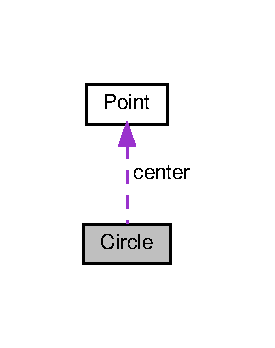
\includegraphics[width=132pt]{class_circle__coll__graph}
\end{center}
\end{figure}
\subsection*{Public Member Functions}
\begin{DoxyCompactItemize}
\item 
\hyperlink{class_circle_a7a761c34c5a913be8bc0b05ea0dc327c}{Circle} (\hyperlink{class_point}{Point} \hyperlink{class_circle_a8c4026a5a34d2df1527f019dd456317b}{center}, float \hyperlink{class_circle_a47644132ec8bec0f3a4e8d0e15bcd5d3}{radius})
\begin{DoxyCompactList}\small\item\em \hyperlink{class_circle}{Circle} Default constructor for circle. \end{DoxyCompactList}\item 
\hyperlink{class_point}{Point} \hyperlink{class_circle_a9818ca0bbac64ff447945a8e51ff9319}{get\+Center} () const
\begin{DoxyCompactList}\small\item\em get\+Center getter method for center point \end{DoxyCompactList}\item 
float \hyperlink{class_circle_a95b7dc25d2e9b1e40a189cd83386a12e}{get\+Radius} () const
\begin{DoxyCompactList}\small\item\em get\+Radius getter method for radius of circle \end{DoxyCompactList}\end{DoxyCompactItemize}
\subsection*{Public Attributes}
\begin{DoxyCompactItemize}
\item 
\hyperlink{class_point}{Point} \hyperlink{class_circle_a8c4026a5a34d2df1527f019dd456317b}{center}
\item 
float \hyperlink{class_circle_a47644132ec8bec0f3a4e8d0e15bcd5d3}{radius}
\end{DoxyCompactItemize}


\subsection{Detailed Description}


Definition at line 171 of file Intersect\+Tester.\+h.



\subsection{Constructor \& Destructor Documentation}
\mbox{\Hypertarget{class_circle_a7a761c34c5a913be8bc0b05ea0dc327c}\label{class_circle_a7a761c34c5a913be8bc0b05ea0dc327c}} 
\index{Circle@{Circle}!Circle@{Circle}}
\index{Circle@{Circle}!Circle@{Circle}}
\subsubsection{\texorpdfstring{Circle()}{Circle()}}
{\footnotesize\ttfamily Circle\+::\+Circle (\begin{DoxyParamCaption}\item[{\hyperlink{class_point}{Point}}]{center,  }\item[{float}]{radius }\end{DoxyParamCaption})\hspace{0.3cm}{\ttfamily [inline]}}



\hyperlink{class_circle}{Circle} Default constructor for circle. 


\begin{DoxyParams}{Parameters}
{\em center} & center point of the circle \\
\hline
{\em radius} & the radius of the circle (distance from center to edge) \\
\hline
\end{DoxyParams}


Definition at line 180 of file Intersect\+Tester.\+h.


\begin{DoxyCode}
181     \{
182         this->center = \hyperlink{class_circle_a8c4026a5a34d2df1527f019dd456317b}{center};
183         this->\hyperlink{class_circle_a47644132ec8bec0f3a4e8d0e15bcd5d3}{radius} = \hyperlink{class_circle_a47644132ec8bec0f3a4e8d0e15bcd5d3}{radius};
184     \}
\end{DoxyCode}


\subsection{Member Function Documentation}
\mbox{\Hypertarget{class_circle_a9818ca0bbac64ff447945a8e51ff9319}\label{class_circle_a9818ca0bbac64ff447945a8e51ff9319}} 
\index{Circle@{Circle}!get\+Center@{get\+Center}}
\index{get\+Center@{get\+Center}!Circle@{Circle}}
\subsubsection{\texorpdfstring{get\+Center()}{getCenter()}}
{\footnotesize\ttfamily \hyperlink{class_point}{Point} Circle\+::get\+Center (\begin{DoxyParamCaption}{ }\end{DoxyParamCaption}) const\hspace{0.3cm}{\ttfamily [inline]}}



get\+Center getter method for center point 

\begin{DoxyReturn}{Returns}
center 
\end{DoxyReturn}


Definition at line 189 of file Intersect\+Tester.\+h.


\begin{DoxyCode}
189 \{ \textcolor{keywordflow}{return} \hyperlink{class_circle_a8c4026a5a34d2df1527f019dd456317b}{center}; \}
\end{DoxyCode}
\mbox{\Hypertarget{class_circle_a95b7dc25d2e9b1e40a189cd83386a12e}\label{class_circle_a95b7dc25d2e9b1e40a189cd83386a12e}} 
\index{Circle@{Circle}!get\+Radius@{get\+Radius}}
\index{get\+Radius@{get\+Radius}!Circle@{Circle}}
\subsubsection{\texorpdfstring{get\+Radius()}{getRadius()}}
{\footnotesize\ttfamily float Circle\+::get\+Radius (\begin{DoxyParamCaption}{ }\end{DoxyParamCaption}) const\hspace{0.3cm}{\ttfamily [inline]}}



get\+Radius getter method for radius of circle 

\begin{DoxyReturn}{Returns}
radius 
\end{DoxyReturn}


Definition at line 194 of file Intersect\+Tester.\+h.


\begin{DoxyCode}
194 \{ \textcolor{keywordflow}{return} \hyperlink{class_circle_a47644132ec8bec0f3a4e8d0e15bcd5d3}{radius}; \}
\end{DoxyCode}


\subsection{Member Data Documentation}
\mbox{\Hypertarget{class_circle_a8c4026a5a34d2df1527f019dd456317b}\label{class_circle_a8c4026a5a34d2df1527f019dd456317b}} 
\index{Circle@{Circle}!center@{center}}
\index{center@{center}!Circle@{Circle}}
\subsubsection{\texorpdfstring{center}{center}}
{\footnotesize\ttfamily \hyperlink{class_point}{Point} Circle\+::center}



Definition at line 173 of file Intersect\+Tester.\+h.

\mbox{\Hypertarget{class_circle_a47644132ec8bec0f3a4e8d0e15bcd5d3}\label{class_circle_a47644132ec8bec0f3a4e8d0e15bcd5d3}} 
\index{Circle@{Circle}!radius@{radius}}
\index{radius@{radius}!Circle@{Circle}}
\subsubsection{\texorpdfstring{radius}{radius}}
{\footnotesize\ttfamily float Circle\+::radius}



Definition at line 174 of file Intersect\+Tester.\+h.



The documentation for this class was generated from the following file\+:\begin{DoxyCompactItemize}
\item 
/home/liam/\+Projects/\+Intersection\+Tester\+G\+U\+I/\+Intersect\+Tester/\hyperlink{_intersect_tester_8h}{Intersect\+Tester.\+h}\end{DoxyCompactItemize}

\hypertarget{class_intersect_tester}{}\section{Intersect\+Tester Class Reference}
\label{class_intersect_tester}\index{Intersect\+Tester@{Intersect\+Tester}}


{\ttfamily \#include $<$Intersect\+Tester.\+h$>$}

\subsection*{Public Member Functions}
\begin{DoxyCompactItemize}
\item 
\hyperlink{class_intersect_tester_a2c6c76bd440dde9b8d158b4c37b174f8}{Intersect\+Tester} ()
\end{DoxyCompactItemize}
\subsection*{Static Public Member Functions}
\begin{DoxyCompactItemize}
\item 
static bool \hyperlink{class_intersect_tester_a7710e17ff7d2e229059f23b9429213f5}{is\+Intersecting} (\hyperlink{class_point}{Point} a, \hyperlink{class_point}{Point} b)
\begin{DoxyCompactList}\small\item\em \hyperlink{class_intersect_tester_a7710e17ff7d2e229059f23b9429213f5}{Intersect\+Tester\+::is\+Intersecting} checks if the two points sit on each other. \end{DoxyCompactList}\item 
static bool \hyperlink{class_intersect_tester_acc62b7619356707ae3295e2fab1694ae}{is\+Intersecting} (\hyperlink{class_point}{Point} p, \hyperlink{class_line_segment}{Line\+Segment} ls)
\begin{DoxyCompactList}\small\item\em \hyperlink{class_intersect_tester_a7710e17ff7d2e229059f23b9429213f5}{Intersect\+Tester\+::is\+Intersecting} calls is\+Point\+On\+Line\+Segment  \hyperlink{class_intersect_tester_a95ba0d50e91eb8559aa3c6a4dc0d4c0f}{Intersect\+Tester\+::is\+Point\+On\+Line\+Segment}. \end{DoxyCompactList}\item 
static bool \hyperlink{class_intersect_tester_a12df0518a663c87dcfcc299e9cd6c07f}{is\+Intersecting} (\hyperlink{class_point}{Point} p, \hyperlink{class_circle}{Circle} c)
\begin{DoxyCompactList}\small\item\em \hyperlink{class_intersect_tester_a7710e17ff7d2e229059f23b9429213f5}{Intersect\+Tester\+::is\+Intersecting} calls is\+Point\+On\+Circle  \hyperlink{class_intersect_tester_a1adb6abbf2f6454b48be18cf5eb69333}{Intersect\+Tester\+::is\+Point\+On\+Circle}. \end{DoxyCompactList}\item 
static bool \hyperlink{class_intersect_tester_afd66862467239ef2fd7c79114c960dc6}{is\+Intersecting} (\hyperlink{class_point}{Point} p, \hyperlink{class_triangle}{Triangle} t)
\begin{DoxyCompactList}\small\item\em \hyperlink{class_intersect_tester_a7710e17ff7d2e229059f23b9429213f5}{Intersect\+Tester\+::is\+Intersecting} calls is\+Point\+On\+Triangle  \hyperlink{class_intersect_tester_a04fb92f5e4c68c3f3a91321b94c6011f}{Intersect\+Tester\+::is\+Point\+On\+Triangle}. \end{DoxyCompactList}\item 
static bool \hyperlink{class_intersect_tester_a29619798894f9997823c27e73f53236d}{is\+Intersecting} (\hyperlink{class_point}{Point} p, \hyperlink{class_a_a_b_b}{A\+A\+BB} a)
\begin{DoxyCompactList}\small\item\em \hyperlink{class_intersect_tester_a7710e17ff7d2e229059f23b9429213f5}{Intersect\+Tester\+::is\+Intersecting} calls is\+Point\+On\+A\+A\+BB  \hyperlink{class_intersect_tester_a04fb92f5e4c68c3f3a91321b94c6011f}{Intersect\+Tester\+::is\+Point\+On\+Triangle}. \end{DoxyCompactList}\item 
static bool \hyperlink{class_intersect_tester_a7984196b3e057a2c02a8f2a8d55847e0}{is\+Intersecting} (\hyperlink{class_line_segment}{Line\+Segment} a, \hyperlink{class_line_segment}{Line\+Segment} b)
\begin{DoxyCompactList}\small\item\em \hyperlink{class_intersect_tester_a7710e17ff7d2e229059f23b9429213f5}{Intersect\+Tester\+::is\+Intersecting} calls are\+Line\+Segments\+Intersecting  \hyperlink{class_intersect_tester_a0552b121b444528907c1958c02fb217b}{Intersect\+Tester\+::are\+Line\+Segments\+Intersecting}. \end{DoxyCompactList}\item 
static bool \hyperlink{class_intersect_tester_ab2cc7dc060f09e9bf33b197de8ca6f16}{is\+Intersecting} (\hyperlink{class_line_segment}{Line\+Segment} a, \hyperlink{class_circle}{Circle} c)
\begin{DoxyCompactList}\small\item\em \hyperlink{class_intersect_tester_a7710e17ff7d2e229059f23b9429213f5}{Intersect\+Tester\+::is\+Intersecting} calls are\+Line\+Segment\+And\+Circle\+Intersecting  \hyperlink{class_intersect_tester_a36c9fcad6ad5607f5a47369aeb2b57c3}{Intersect\+Tester\+::are\+Line\+Segment\+And\+Circle\+Intersecting}. \end{DoxyCompactList}\item 
static bool \hyperlink{class_intersect_tester_aa7f33e35eaa5d3662fc8a57e99eff82f}{is\+Intersecting} (\hyperlink{class_line_segment}{Line\+Segment} ls, \hyperlink{class_triangle}{Triangle} t)
\begin{DoxyCompactList}\small\item\em \hyperlink{class_intersect_tester_a7710e17ff7d2e229059f23b9429213f5}{Intersect\+Tester\+::is\+Intersecting} calls does\+Line\+Segment\+Intersect\+Triangle  \hyperlink{class_intersect_tester_a7e7603c33cc5921adb9d0d24eb76ebc9}{Intersect\+Tester\+::does\+Line\+Segment\+Intersect\+Triangle}. \end{DoxyCompactList}\item 
static bool \hyperlink{class_intersect_tester_a6caf298c7e2e46a9b00f68ce9554a5eb}{is\+Intersecting} (\hyperlink{class_line_segment}{Line\+Segment} ls, \hyperlink{class_a_a_b_b}{A\+A\+BB} a)
\begin{DoxyCompactList}\small\item\em \hyperlink{class_intersect_tester_a7710e17ff7d2e229059f23b9429213f5}{Intersect\+Tester\+::is\+Intersecting} calls does\+Line\+Segment\+Intersect\+A\+A\+BB  \hyperlink{class_intersect_tester_a817105ec3f73e20066121d7d9d85a3ae}{Intersect\+Tester\+::does\+Line\+Segment\+Intersect\+A\+A\+BB}. \end{DoxyCompactList}\item 
static bool \hyperlink{class_intersect_tester_a3f908e959ef38b2591582b8796ed2efd}{is\+Intersecting} (\hyperlink{class_circle}{Circle} a, \hyperlink{class_circle}{Circle} b)
\begin{DoxyCompactList}\small\item\em \hyperlink{class_intersect_tester_a7710e17ff7d2e229059f23b9429213f5}{Intersect\+Tester\+::is\+Intersecting} calls do\+Circles\+Intersect  \hyperlink{class_intersect_tester_a5ce26d69bdb46983fb96516c8a8e1b55}{Intersect\+Tester\+::do\+Circles\+Intersect}. \end{DoxyCompactList}\item 
static bool \hyperlink{class_intersect_tester_a76f351cdf60b75daf6a4a1e7240c1f3d}{is\+Intersecting} (\hyperlink{class_circle}{Circle} c, \hyperlink{class_triangle}{Triangle} t)
\begin{DoxyCompactList}\small\item\em \hyperlink{class_intersect_tester_a7710e17ff7d2e229059f23b9429213f5}{Intersect\+Tester\+::is\+Intersecting} calls does\+Circle\+Intersect\+Triangle  \hyperlink{class_intersect_tester_a4a2f8f6f66be1f1d432c3e04e919273f}{Intersect\+Tester\+::does\+Circle\+Intersect\+Triangle}. \end{DoxyCompactList}\item 
static bool \hyperlink{class_intersect_tester_afe557ee5f9e2da763c430cbbad44162e}{is\+Intersecting} (\hyperlink{class_circle}{Circle} c, \hyperlink{class_a_a_b_b}{A\+A\+BB} a)
\begin{DoxyCompactList}\small\item\em \hyperlink{class_intersect_tester_a7710e17ff7d2e229059f23b9429213f5}{Intersect\+Tester\+::is\+Intersecting} calls do\+Circleand\+A\+A\+B\+B\+Intersect  \hyperlink{class_intersect_tester_af76b72861b57c630e7c54ad9449a2d27}{Intersect\+Tester\+::do\+Circleand\+A\+A\+B\+B\+Intersect}. \end{DoxyCompactList}\item 
static bool \hyperlink{class_intersect_tester_a7195f2152c0c36590c2cdbd0e7365a3b}{is\+Intersecting} (\hyperlink{class_triangle}{Triangle} a, \hyperlink{class_triangle}{Triangle} b)
\begin{DoxyCompactList}\small\item\em \hyperlink{class_intersect_tester_a7710e17ff7d2e229059f23b9429213f5}{Intersect\+Tester\+::is\+Intersecting} calls do\+Triangles\+Intersect  \hyperlink{class_intersect_tester_a42709665c17cf203a7157466fdccd10f}{Intersect\+Tester\+::do\+Triangles\+Intersect}. \end{DoxyCompactList}\item 
static bool \hyperlink{class_intersect_tester_a7676eefb6df137a07551f4b49f8926a6}{is\+Intersecting} (\hyperlink{class_triangle}{Triangle} t, \hyperlink{class_a_a_b_b}{A\+A\+BB} a)
\begin{DoxyCompactList}\small\item\em \hyperlink{class_intersect_tester_a7710e17ff7d2e229059f23b9429213f5}{Intersect\+Tester\+::is\+Intersecting} calls do\+Triangle\+And\+A\+A\+B\+B\+Intersect  \hyperlink{class_intersect_tester_acb2dbd261f6351d83cf7471a972b5b52}{Intersect\+Tester\+::do\+Triangle\+And\+A\+A\+B\+B\+Intersect}. \end{DoxyCompactList}\item 
static bool \hyperlink{class_intersect_tester_a3996af79d5b862299a88dbb5705da88f}{is\+Intersecting} (\hyperlink{class_a_a_b_b}{A\+A\+BB} a, \hyperlink{class_a_a_b_b}{A\+A\+BB} b)
\begin{DoxyCompactList}\small\item\em \hyperlink{class_intersect_tester_a7710e17ff7d2e229059f23b9429213f5}{Intersect\+Tester\+::is\+Intersecting} calls are\+Boxes\+Intersecting  \hyperlink{class_intersect_tester_aff69bf4a84e714029204496c2efb0b3b}{Intersect\+Tester\+::are\+Boxes\+Intersecting}. \end{DoxyCompactList}\item 
static float \hyperlink{class_intersect_tester_a8eea20bc180b49008d29002fc4e2c7cf}{distance\+Between\+Points} (\hyperlink{class_point}{Point} a, \hyperlink{class_point}{Point} b)
\begin{DoxyCompactList}\small\item\em distance\+Between\+Points calculates the distance between two points. \end{DoxyCompactList}\item 
static float \hyperlink{class_intersect_tester_a1b966d15da1de1fab5350c8e81e0b70f}{cross\+Product} (\hyperlink{class_point}{Point} a, \hyperlink{class_point}{Point} b, \hyperlink{class_point}{Point} c)
\begin{DoxyCompactList}\small\item\em cross\+Product calculates the cross product of three points \end{DoxyCompactList}\item 
static float \hyperlink{class_intersect_tester_acf0fb2d4e58655d8314b2409a46900c2}{dot\+Product} (\hyperlink{class_point}{Point} a, \hyperlink{class_point}{Point} b, \hyperlink{class_point}{Point} c)
\begin{DoxyCompactList}\small\item\em dot\+Product calculates the dot product of three points \end{DoxyCompactList}\item 
static int \hyperlink{class_intersect_tester_a9d0a30b1831dbf7b80f8e2bfaf1b4a0b}{direction} (\hyperlink{class_point}{Point} a, \hyperlink{class_point}{Point} b, \hyperlink{class_point}{Point} c)
\begin{DoxyCompactList}\small\item\em direction return the sign of the vector of points. \end{DoxyCompactList}\item 
static void \hyperlink{class_intersect_tester_ac837c3469e328c8bb47d08742c304c9a}{set\+Tolerance} (float value)
\begin{DoxyCompactList}\small\item\em set\+Tolerance set the tolerance value for precision tests. \end{DoxyCompactList}\item 
static \hyperlink{class_point}{Point} \hyperlink{class_intersect_tester_a6bb20d4839643fbfd53a5d4506448a92}{closest\+Point} (\hyperlink{class_line_segment}{Line\+Segment} ls, \hyperlink{class_point}{Point} c)
\begin{DoxyCompactList}\small\item\em closest\+Point returns the closest point on a line segment to \hyperlink{class_point}{Point} c. \end{DoxyCompactList}\end{DoxyCompactItemize}
\subsection*{Private Member Functions}
\begin{DoxyCompactItemize}
\item 
bool \hyperlink{class_intersect_tester_af4b47b5b70e769205f6b113cb054f961}{is\+Point\+On\+Line\+Segment\+Old} (\hyperlink{class_point}{Point} p, \hyperlink{class_line_segment}{Line\+Segment} ls)
\end{DoxyCompactItemize}
\subsection*{Static Private Member Functions}
\begin{DoxyCompactItemize}
\item 
static bool \hyperlink{class_intersect_tester_a95ba0d50e91eb8559aa3c6a4dc0d4c0f}{is\+Point\+On\+Line\+Segment} (\hyperlink{class_point}{Point} p, \hyperlink{class_line_segment}{Line\+Segment} ls)
\begin{DoxyCompactList}\small\item\em \hyperlink{class_intersect_tester_a95ba0d50e91eb8559aa3c6a4dc0d4c0f}{Intersect\+Tester\+::is\+Point\+On\+Line\+Segment} used to check whether a coordinate point (p) intersects with a line (ls). \end{DoxyCompactList}\item 
static bool \hyperlink{class_intersect_tester_a1adb6abbf2f6454b48be18cf5eb69333}{is\+Point\+On\+Circle} (\hyperlink{class_point}{Point} p, \hyperlink{class_circle}{Circle} c)
\begin{DoxyCompactList}\small\item\em is\+Point\+On\+Circle Tested by checking the distance between the point, and the center of the circle, if the distance is less than or equal to the radius, the point is within the circle. \end{DoxyCompactList}\item 
static bool \hyperlink{class_intersect_tester_a04fb92f5e4c68c3f3a91321b94c6011f}{is\+Point\+On\+Triangle} (\hyperlink{class_point}{Point} p, \hyperlink{class_triangle}{Triangle} t)
\begin{DoxyCompactList}\small\item\em is\+Point\+On\+Triangle In order for a point to sit inside a triangle we must check the crossproduct for a direction. if all crossproducts move in the same direction, then the point sits in the triangle. We also check edge cases using previous tests point-\/to-\/line, and point-\/to-\/point. \end{DoxyCompactList}\item 
static bool \hyperlink{class_intersect_tester_a7d951e17cc8d244ea34b3e75d53e5bca}{is\+Point\+On\+A\+A\+BB} (\hyperlink{class_point}{Point} p, \hyperlink{class_a_a_b_b}{A\+A\+BB} a)
\begin{DoxyCompactList}\small\item\em is\+Point\+On\+A\+A\+BB We test the null hypothesis. If the X axis, or the Y axis fall outside of the axes range of the bounding box, the we know this is false. Otherwise it is true. \end{DoxyCompactList}\item 
static bool \hyperlink{class_intersect_tester_a0552b121b444528907c1958c02fb217b}{are\+Line\+Segments\+Intersecting} (\hyperlink{class_line_segment}{Line\+Segment} a, \hyperlink{class_line_segment}{Line\+Segment} b)
\begin{DoxyCompactList}\small\item\em are\+Line\+Segments\+Intersecting we check the vector direction between the points. If the both ends of the line segment sit on seperate sides of the opposing line,than they intersect. Otherwise we also check if the lines sit on top of each other. \end{DoxyCompactList}\item 
static bool \hyperlink{class_intersect_tester_a36c9fcad6ad5607f5a47369aeb2b57c3}{are\+Line\+Segment\+And\+Circle\+Intersecting} (\hyperlink{class_line_segment}{Line\+Segment} a, \hyperlink{class_circle}{Circle} c)
\begin{DoxyCompactList}\small\item\em are\+Line\+Segment\+And\+Circle\+Intersecting We calculate the closest point between the line and the circle\textquotesingle{}s center. If the closest point falls on the line segment and the distance is less than the radius, the two intersect. \end{DoxyCompactList}\item 
static bool \hyperlink{class_intersect_tester_a7e7603c33cc5921adb9d0d24eb76ebc9}{does\+Line\+Segment\+Intersect\+Triangle} (\hyperlink{class_line_segment}{Line\+Segment} a, \hyperlink{class_triangle}{Triangle} t)
\begin{DoxyCompactList}\small\item\em does\+Line\+Segment\+Intersect\+Triangle we test the line segment against each edge of the triangle. If any of the lines intersect, than we know the line and triangle intersect. \end{DoxyCompactList}\item 
static bool \hyperlink{class_intersect_tester_a817105ec3f73e20066121d7d9d85a3ae}{does\+Line\+Segment\+Intersect\+A\+A\+BB} (\hyperlink{class_line_segment}{Line\+Segment} ls, \hyperlink{class_a_a_b_b}{A\+A\+BB} a)
\begin{DoxyCompactList}\small\item\em does\+Line\+Segment\+Intersect\+A\+A\+BB We first check if either point lies of the line segment fall inside the box, if not, we test every line-\/to-\/line intersection. If any return true, we know the \hyperlink{class_line_segment}{Line\+Segment} and \hyperlink{class_a_a_b_b}{A\+A\+BB} intersect \end{DoxyCompactList}\item 
static bool \hyperlink{class_intersect_tester_a5ce26d69bdb46983fb96516c8a8e1b55}{do\+Circles\+Intersect} (\hyperlink{class_circle}{Circle} a, \hyperlink{class_circle}{Circle} b)
\begin{DoxyCompactList}\small\item\em do\+Circles\+Intersect we calculate the distance between points. If the distance is less than the combined radius, the two circles intersect. \end{DoxyCompactList}\item 
static bool \hyperlink{class_intersect_tester_a4a2f8f6f66be1f1d432c3e04e919273f}{does\+Circle\+Intersect\+Triangle} (\hyperlink{class_circle}{Circle} c, \hyperlink{class_triangle}{Triangle} t)
\begin{DoxyCompactList}\small\item\em does\+Circle\+Intersect\+Triangle we test if the circle\textquotesingle{}s center point sits in the triangle, if not we also check if any triangle edge intersects with the circle. If any of these are true, we know the two objects intersect. \end{DoxyCompactList}\item 
static bool \hyperlink{class_intersect_tester_af76b72861b57c630e7c54ad9449a2d27}{do\+Circleand\+A\+A\+B\+B\+Intersect} (\hyperlink{class_circle}{Circle} c, \hyperlink{class_a_a_b_b}{A\+A\+BB} a)
\begin{DoxyCompactList}\small\item\em do\+Circleand\+A\+A\+B\+B\+Intersect we test the circle\textquotesingle{}s center, using a point-\/to-\/box, and point-\/to-\/line tests. If any are true, we know the two intersect. \end{DoxyCompactList}\item 
static bool \hyperlink{class_intersect_tester_a42709665c17cf203a7157466fdccd10f}{do\+Triangles\+Intersect} (\hyperlink{class_triangle}{Triangle} a, \hyperlink{class_triangle}{Triangle} b)
\begin{DoxyCompactList}\small\item\em do\+Triangles\+Intersect we test the edges of the triangles against each other. If any are true, we know the triangles intersect \end{DoxyCompactList}\item 
static bool \hyperlink{class_intersect_tester_acb2dbd261f6351d83cf7471a972b5b52}{do\+Triangle\+And\+A\+A\+B\+B\+Intersect} (\hyperlink{class_triangle}{Triangle} t, \hyperlink{class_a_a_b_b}{A\+A\+BB} a)
\begin{DoxyCompactList}\small\item\em do\+Triangle\+And\+A\+A\+B\+B\+Intersect we test the edges of the triangle and \hyperlink{class_a_a_b_b}{A\+A\+BB} against each other. If any are true, we know the two intersect \end{DoxyCompactList}\item 
static bool \hyperlink{class_intersect_tester_aff69bf4a84e714029204496c2efb0b3b}{are\+Boxes\+Intersecting} (\hyperlink{class_a_a_b_b}{A\+A\+BB} a, \hyperlink{class_a_a_b_b}{A\+A\+BB} b)
\begin{DoxyCompactList}\small\item\em are\+Boxes\+Intersecting the axis-\/aligned box test is similar to the point test. We use the null hypothesis. If the X dimension extents of \hyperlink{class_a_a_b_b}{A\+A\+BB} 2 do not fall into the extents of \hyperlink{class_a_a_b_b}{A\+A\+BB} 1, then we know that it is not possible for the boxes to intersect. We can make the same assumption for the Y axis. If both the X and Y axes of \hyperlink{class_a_a_b_b}{A\+A\+BB} 2 can be found in \hyperlink{class_a_a_b_b}{A\+A\+BB} 1, then we know that they intersect. \end{DoxyCompactList}\end{DoxyCompactItemize}
\subsection*{Static Private Attributes}
\begin{DoxyCompactItemize}
\item 
static float \hyperlink{class_intersect_tester_a50c5d2e177394644ceee23c700a541fd}{tolerance} = std\+::numeric\+\_\+limits$<$float$>$\+::epsilon()
\end{DoxyCompactItemize}


\subsection{Detailed Description}


Definition at line 199 of file Intersect\+Tester.\+h.



\subsection{Constructor \& Destructor Documentation}
\mbox{\Hypertarget{class_intersect_tester_a2c6c76bd440dde9b8d158b4c37b174f8}\label{class_intersect_tester_a2c6c76bd440dde9b8d158b4c37b174f8}} 
\index{Intersect\+Tester@{Intersect\+Tester}!Intersect\+Tester@{Intersect\+Tester}}
\index{Intersect\+Tester@{Intersect\+Tester}!Intersect\+Tester@{Intersect\+Tester}}
\subsubsection{\texorpdfstring{Intersect\+Tester()}{IntersectTester()}}
{\footnotesize\ttfamily Intersect\+Tester\+::\+Intersect\+Tester (\begin{DoxyParamCaption}{ }\end{DoxyParamCaption})}



\subsection{Member Function Documentation}
\mbox{\Hypertarget{class_intersect_tester_aff69bf4a84e714029204496c2efb0b3b}\label{class_intersect_tester_aff69bf4a84e714029204496c2efb0b3b}} 
\index{Intersect\+Tester@{Intersect\+Tester}!are\+Boxes\+Intersecting@{are\+Boxes\+Intersecting}}
\index{are\+Boxes\+Intersecting@{are\+Boxes\+Intersecting}!Intersect\+Tester@{Intersect\+Tester}}
\subsubsection{\texorpdfstring{are\+Boxes\+Intersecting()}{areBoxesIntersecting()}}
{\footnotesize\ttfamily bool Intersect\+Tester\+::are\+Boxes\+Intersecting (\begin{DoxyParamCaption}\item[{\hyperlink{class_a_a_b_b}{A\+A\+BB}}]{a,  }\item[{\hyperlink{class_a_a_b_b}{A\+A\+BB}}]{b }\end{DoxyParamCaption})\hspace{0.3cm}{\ttfamily [static]}, {\ttfamily [private]}}



are\+Boxes\+Intersecting the axis-\/aligned box test is similar to the point test. We use the null hypothesis. If the X dimension extents of \hyperlink{class_a_a_b_b}{A\+A\+BB} 2 do not fall into the extents of \hyperlink{class_a_a_b_b}{A\+A\+BB} 1, then we know that it is not possible for the boxes to intersect. We can make the same assumption for the Y axis. If both the X and Y axes of \hyperlink{class_a_a_b_b}{A\+A\+BB} 2 can be found in \hyperlink{class_a_a_b_b}{A\+A\+BB} 1, then we know that they intersect. 


\begin{DoxyParams}{Parameters}
{\em a} & \hyperlink{class_a_a_b_b}{A\+A\+BB} 1 \\
\hline
{\em b} & \hyperlink{class_a_a_b_b}{A\+A\+BB} 2 \\
\hline
\end{DoxyParams}
\begin{DoxyReturn}{Returns}

\end{DoxyReturn}


Definition at line 239 of file Intersect\+Tester.\+cpp.


\begin{DoxyCode}
240 \{
241     \textcolor{keywordflow}{return} a.\hyperlink{class_a_a_b_b_a62290d3f27644484f2df17c42cd1bfd5}{intersects}(b);
242 \}
\end{DoxyCode}
\mbox{\Hypertarget{class_intersect_tester_a36c9fcad6ad5607f5a47369aeb2b57c3}\label{class_intersect_tester_a36c9fcad6ad5607f5a47369aeb2b57c3}} 
\index{Intersect\+Tester@{Intersect\+Tester}!are\+Line\+Segment\+And\+Circle\+Intersecting@{are\+Line\+Segment\+And\+Circle\+Intersecting}}
\index{are\+Line\+Segment\+And\+Circle\+Intersecting@{are\+Line\+Segment\+And\+Circle\+Intersecting}!Intersect\+Tester@{Intersect\+Tester}}
\subsubsection{\texorpdfstring{are\+Line\+Segment\+And\+Circle\+Intersecting()}{areLineSegmentAndCircleIntersecting()}}
{\footnotesize\ttfamily bool Intersect\+Tester\+::are\+Line\+Segment\+And\+Circle\+Intersecting (\begin{DoxyParamCaption}\item[{\hyperlink{class_line_segment}{Line\+Segment}}]{a,  }\item[{\hyperlink{class_circle}{Circle}}]{c }\end{DoxyParamCaption})\hspace{0.3cm}{\ttfamily [static]}, {\ttfamily [private]}}



are\+Line\+Segment\+And\+Circle\+Intersecting We calculate the closest point between the line and the circle\textquotesingle{}s center. If the closest point falls on the line segment and the distance is less than the radius, the two intersect. 


\begin{DoxyParams}{Parameters}
{\em a} & \hyperlink{class_line_segment}{Line\+Segment} \\
\hline
{\em c} & \hyperlink{class_circle}{Circle} \\
\hline
\end{DoxyParams}
\begin{DoxyReturn}{Returns}
if linesegment and circle intersect, return true, otherwise return false. 
\end{DoxyReturn}


Definition at line 122 of file Intersect\+Tester.\+cpp.


\begin{DoxyCode}
123 \{
124     \textcolor{keywordflow}{if}( \hyperlink{class_intersect_tester_a7710e17ff7d2e229059f23b9429213f5}{isIntersecting}( a.\hyperlink{class_line_segment_afcff6bd5f6a3073a44f7b21db0be876f}{getStart}(), c) || \hyperlink{class_intersect_tester_a7710e17ff7d2e229059f23b9429213f5}{isIntersecting}(a.
      \hyperlink{class_line_segment_a7b05f883c369b950e61009edfafbbd0e}{getEnd}(), c) )
125         \textcolor{keywordflow}{return} \textcolor{keyword}{true};
126 
127     \hyperlink{class_point}{Point} closest = \hyperlink{class_intersect_tester_a6bb20d4839643fbfd53a5d4506448a92}{closestPoint}(a, c.\hyperlink{class_circle_a9818ca0bbac64ff447945a8e51ff9319}{getCenter}());
128 
129     \textcolor{keywordflow}{if} (!\hyperlink{class_intersect_tester_a7710e17ff7d2e229059f23b9429213f5}{isIntersecting}(closest,a))
130         \textcolor{keywordflow}{return} \textcolor{keyword}{false};
131 
132     \textcolor{keywordtype}{float} distTest = \hyperlink{class_intersect_tester_a8eea20bc180b49008d29002fc4e2c7cf}{distanceBetweenPoints}( closest, c.
      \hyperlink{class_circle_a9818ca0bbac64ff447945a8e51ff9319}{getCenter}() );
133     \textcolor{keywordflow}{if}( distTest <= c.\hyperlink{class_circle_a95b7dc25d2e9b1e40a189cd83386a12e}{getRadius}() )
134         \textcolor{keywordflow}{return} \textcolor{keyword}{true};
135     \textcolor{keywordflow}{return} \textcolor{keyword}{false};
136 \}
\end{DoxyCode}
\mbox{\Hypertarget{class_intersect_tester_a0552b121b444528907c1958c02fb217b}\label{class_intersect_tester_a0552b121b444528907c1958c02fb217b}} 
\index{Intersect\+Tester@{Intersect\+Tester}!are\+Line\+Segments\+Intersecting@{are\+Line\+Segments\+Intersecting}}
\index{are\+Line\+Segments\+Intersecting@{are\+Line\+Segments\+Intersecting}!Intersect\+Tester@{Intersect\+Tester}}
\subsubsection{\texorpdfstring{are\+Line\+Segments\+Intersecting()}{areLineSegmentsIntersecting()}}
{\footnotesize\ttfamily bool Intersect\+Tester\+::are\+Line\+Segments\+Intersecting (\begin{DoxyParamCaption}\item[{\hyperlink{class_line_segment}{Line\+Segment}}]{a,  }\item[{\hyperlink{class_line_segment}{Line\+Segment}}]{b }\end{DoxyParamCaption})\hspace{0.3cm}{\ttfamily [static]}, {\ttfamily [private]}}



are\+Line\+Segments\+Intersecting we check the vector direction between the points. If the both ends of the line segment sit on seperate sides of the opposing line,than they intersect. Otherwise we also check if the lines sit on top of each other. 


\begin{DoxyParams}{Parameters}
{\em a} & \hyperlink{class_line_segment}{Line\+Segment} a \\
\hline
{\em b} & \hyperlink{class_line_segment}{Line\+Segment} b \\
\hline
\end{DoxyParams}
\begin{DoxyReturn}{Returns}
if line segments intersect, return true, otherwise return false 
\end{DoxyReturn}


Definition at line 100 of file Intersect\+Tester.\+cpp.


\begin{DoxyCode}
101 \{
102     \textcolor{keywordtype}{int} or1, or2, or3, or4;
103     or1 = \hyperlink{class_intersect_tester_a9d0a30b1831dbf7b80f8e2bfaf1b4a0b}{direction}( a.\hyperlink{class_line_segment_afcff6bd5f6a3073a44f7b21db0be876f}{getStart}(), a.\hyperlink{class_line_segment_a7b05f883c369b950e61009edfafbbd0e}{getEnd}(), b.\hyperlink{class_line_segment_afcff6bd5f6a3073a44f7b21db0be876f}{getStart}() );
104     or2 = \hyperlink{class_intersect_tester_a9d0a30b1831dbf7b80f8e2bfaf1b4a0b}{direction}( a.\hyperlink{class_line_segment_afcff6bd5f6a3073a44f7b21db0be876f}{getStart}(), a.\hyperlink{class_line_segment_a7b05f883c369b950e61009edfafbbd0e}{getEnd}(), b.\hyperlink{class_line_segment_a7b05f883c369b950e61009edfafbbd0e}{getEnd}() );
105     or3 = \hyperlink{class_intersect_tester_a9d0a30b1831dbf7b80f8e2bfaf1b4a0b}{direction}( b.\hyperlink{class_line_segment_afcff6bd5f6a3073a44f7b21db0be876f}{getStart}(), b.\hyperlink{class_line_segment_a7b05f883c369b950e61009edfafbbd0e}{getEnd}(), a.\hyperlink{class_line_segment_afcff6bd5f6a3073a44f7b21db0be876f}{getStart}() );
106     or4 = \hyperlink{class_intersect_tester_a9d0a30b1831dbf7b80f8e2bfaf1b4a0b}{direction}( b.\hyperlink{class_line_segment_afcff6bd5f6a3073a44f7b21db0be876f}{getStart}(), b.\hyperlink{class_line_segment_a7b05f883c369b950e61009edfafbbd0e}{getEnd}(), a.\hyperlink{class_line_segment_a7b05f883c369b950e61009edfafbbd0e}{getEnd}() );
107 
108     \textcolor{keywordflow}{if} (or1 != or2 && or3 != or4 )
109         \textcolor{keywordflow}{return} \textcolor{keyword}{true};
110     \textcolor{keywordflow}{if}( or1 == 0 && \hyperlink{class_intersect_tester_a7710e17ff7d2e229059f23b9429213f5}{isIntersecting}( b.\hyperlink{class_line_segment_afcff6bd5f6a3073a44f7b21db0be876f}{getStart}(), a ) )
111         \textcolor{keywordflow}{return} \textcolor{keyword}{true};
112     \textcolor{keywordflow}{if}( or2 == 0 && \hyperlink{class_intersect_tester_a7710e17ff7d2e229059f23b9429213f5}{isIntersecting}( a.\hyperlink{class_line_segment_afcff6bd5f6a3073a44f7b21db0be876f}{getStart}(), b ) )
113         \textcolor{keywordflow}{return} \textcolor{keyword}{true};
114     \textcolor{keywordflow}{if}( or3 == 0 && \hyperlink{class_intersect_tester_a7710e17ff7d2e229059f23b9429213f5}{isIntersecting}( b.\hyperlink{class_line_segment_a7b05f883c369b950e61009edfafbbd0e}{getEnd}(), a ) )
115         \textcolor{keywordflow}{return} \textcolor{keyword}{true};
116     \textcolor{keywordflow}{if}( or4 == 0 && \hyperlink{class_intersect_tester_a7710e17ff7d2e229059f23b9429213f5}{isIntersecting}( a.\hyperlink{class_line_segment_a7b05f883c369b950e61009edfafbbd0e}{getEnd}(), b ) )
117         \textcolor{keywordflow}{return} \textcolor{keyword}{true};
118 
119     \textcolor{keywordflow}{return} \textcolor{keyword}{false};
120 \}
\end{DoxyCode}
\mbox{\Hypertarget{class_intersect_tester_a6bb20d4839643fbfd53a5d4506448a92}\label{class_intersect_tester_a6bb20d4839643fbfd53a5d4506448a92}} 
\index{Intersect\+Tester@{Intersect\+Tester}!closest\+Point@{closest\+Point}}
\index{closest\+Point@{closest\+Point}!Intersect\+Tester@{Intersect\+Tester}}
\subsubsection{\texorpdfstring{closest\+Point()}{closestPoint()}}
{\footnotesize\ttfamily \hyperlink{class_point}{Point} Intersect\+Tester\+::closest\+Point (\begin{DoxyParamCaption}\item[{\hyperlink{class_line_segment}{Line\+Segment}}]{ls,  }\item[{\hyperlink{class_point}{Point}}]{c }\end{DoxyParamCaption})\hspace{0.3cm}{\ttfamily [static]}}



closest\+Point returns the closest point on a line segment to \hyperlink{class_point}{Point} c. 


\begin{DoxyParams}{Parameters}
{\em ls} & \hyperlink{class_line_segment}{Line\+Segment} \\
\hline
{\em c} & \hyperlink{class_point}{Point} \\
\hline
\end{DoxyParams}
\begin{DoxyReturn}{Returns}

\end{DoxyReturn}


Definition at line 288 of file Intersect\+Tester.\+cpp.


\begin{DoxyCode}
289 \{
290     \hyperlink{class_point}{Point} p1 = ls.\hyperlink{class_line_segment_afcff6bd5f6a3073a44f7b21db0be876f}{getStart}();
291     \hyperlink{class_point}{Point} p2 = ls.\hyperlink{class_line_segment_a7b05f883c369b950e61009edfafbbd0e}{getEnd}();
292     \hyperlink{class_point}{Point} p3 = c;
293 
294     \textcolor{keywordtype}{float} distX = (p1.\hyperlink{class_point_a29c44ec7c7279e02629645a06cdaf7d5}{getX}() - p2.\hyperlink{class_point_a29c44ec7c7279e02629645a06cdaf7d5}{getX}());
295     \textcolor{keywordtype}{float} distY = (p1.\hyperlink{class_point_a2371ffadbe245d12a8f556d0a976521b}{getY}() - p2.\hyperlink{class_point_a2371ffadbe245d12a8f556d0a976521b}{getY}());
296 
297     \textcolor{keywordtype}{float} len = sqrt( (distX * distX ) + (distY * distY ) );
298     \textcolor{keywordtype}{float} dot = (\hyperlink{class_intersect_tester_acf0fb2d4e58655d8314b2409a46900c2}{dotProduct}( p3, p1, p2 )) / (len*len);
299 
300     \textcolor{keywordtype}{float} closestX = p1.\hyperlink{class_point_a29c44ec7c7279e02629645a06cdaf7d5}{getX}() + ( dot * fabs( p2.\hyperlink{class_point_a29c44ec7c7279e02629645a06cdaf7d5}{getX}() - p1.\hyperlink{class_point_a29c44ec7c7279e02629645a06cdaf7d5}{getX}() ) );
301     \textcolor{keywordtype}{float} closestY = p1.\hyperlink{class_point_a2371ffadbe245d12a8f556d0a976521b}{getY}() + ( dot * fabs( p2.\hyperlink{class_point_a2371ffadbe245d12a8f556d0a976521b}{getY}() - p1.\hyperlink{class_point_a2371ffadbe245d12a8f556d0a976521b}{getY}() ) );
302     \textcolor{keywordflow}{return} \hyperlink{class_point}{Point}(closestX, closestY);
303 \}
\end{DoxyCode}
\mbox{\Hypertarget{class_intersect_tester_a1b966d15da1de1fab5350c8e81e0b70f}\label{class_intersect_tester_a1b966d15da1de1fab5350c8e81e0b70f}} 
\index{Intersect\+Tester@{Intersect\+Tester}!cross\+Product@{cross\+Product}}
\index{cross\+Product@{cross\+Product}!Intersect\+Tester@{Intersect\+Tester}}
\subsubsection{\texorpdfstring{cross\+Product()}{crossProduct()}}
{\footnotesize\ttfamily float Intersect\+Tester\+::cross\+Product (\begin{DoxyParamCaption}\item[{\hyperlink{class_point}{Point}}]{a,  }\item[{\hyperlink{class_point}{Point}}]{b,  }\item[{\hyperlink{class_point}{Point}}]{c }\end{DoxyParamCaption})\hspace{0.3cm}{\ttfamily [static]}}



cross\+Product calculates the cross product of three points 


\begin{DoxyParams}{Parameters}
{\em a} & \hyperlink{class_point}{Point} \\
\hline
{\em b} & \hyperlink{class_point}{Point} \\
\hline
{\em c} & \hyperlink{class_point}{Point} \\
\hline
\end{DoxyParams}
\begin{DoxyReturn}{Returns}

\end{DoxyReturn}


Definition at line 259 of file Intersect\+Tester.\+cpp.


\begin{DoxyCode}
260 \{
261     \textcolor{keywordflow}{return} ( a.\hyperlink{class_point_a2371ffadbe245d12a8f556d0a976521b}{getY}() - b.\hyperlink{class_point_a2371ffadbe245d12a8f556d0a976521b}{getY}() ) *
262            ( c.\hyperlink{class_point_a29c44ec7c7279e02629645a06cdaf7d5}{getX}() - b.\hyperlink{class_point_a29c44ec7c7279e02629645a06cdaf7d5}{getX}() ) -
263            ( a.\hyperlink{class_point_a29c44ec7c7279e02629645a06cdaf7d5}{getX}() - b.\hyperlink{class_point_a29c44ec7c7279e02629645a06cdaf7d5}{getX}() ) *
264            ( c.\hyperlink{class_point_a2371ffadbe245d12a8f556d0a976521b}{getY}() - b.\hyperlink{class_point_a2371ffadbe245d12a8f556d0a976521b}{getY}() );
265 \}
\end{DoxyCode}
\mbox{\Hypertarget{class_intersect_tester_a9d0a30b1831dbf7b80f8e2bfaf1b4a0b}\label{class_intersect_tester_a9d0a30b1831dbf7b80f8e2bfaf1b4a0b}} 
\index{Intersect\+Tester@{Intersect\+Tester}!direction@{direction}}
\index{direction@{direction}!Intersect\+Tester@{Intersect\+Tester}}
\subsubsection{\texorpdfstring{direction()}{direction()}}
{\footnotesize\ttfamily int Intersect\+Tester\+::direction (\begin{DoxyParamCaption}\item[{\hyperlink{class_point}{Point}}]{a,  }\item[{\hyperlink{class_point}{Point}}]{b,  }\item[{\hyperlink{class_point}{Point}}]{c }\end{DoxyParamCaption})\hspace{0.3cm}{\ttfamily [static]}}



direction return the sign of the vector of points. 


\begin{DoxyParams}{Parameters}
{\em a} & \hyperlink{class_point}{Point} \\
\hline
{\em b} & \hyperlink{class_point}{Point} \\
\hline
{\em c} & \hyperlink{class_point}{Point} \\
\hline
\end{DoxyParams}
\begin{DoxyReturn}{Returns}
returns 1 if positive, -\/1 if negative, and 0 if colinear. 
\end{DoxyReturn}


Definition at line 274 of file Intersect\+Tester.\+cpp.


\begin{DoxyCode}
275 \{
276     \textcolor{keywordtype}{float} dir = ( b.\hyperlink{class_point_a2371ffadbe245d12a8f556d0a976521b}{getY}() - a.\hyperlink{class_point_a2371ffadbe245d12a8f556d0a976521b}{getY}() ) * ( c.\hyperlink{class_point_a29c44ec7c7279e02629645a06cdaf7d5}{getX}() - b.\hyperlink{class_point_a29c44ec7c7279e02629645a06cdaf7d5}{getX}() ) -
277               ( b.\hyperlink{class_point_a29c44ec7c7279e02629645a06cdaf7d5}{getX}() - a.\hyperlink{class_point_a29c44ec7c7279e02629645a06cdaf7d5}{getX}() ) * ( c.\hyperlink{class_point_a2371ffadbe245d12a8f556d0a976521b}{getY}() - b.\hyperlink{class_point_a2371ffadbe245d12a8f556d0a976521b}{getY}() );
278 
279     \textcolor{keywordflow}{if} (dir == 0)
280         \textcolor{keywordflow}{return} 0; \textcolor{comment}{//Colinear}
281     \textcolor{keywordflow}{else} \textcolor{keywordflow}{if} ( dir > 0 )
282         \textcolor{keywordflow}{return} 1; \textcolor{comment}{//Clockwise}
283 
284     \textcolor{keywordflow}{return} -1; \textcolor{comment}{//Anti-clockwise}
285 \}
\end{DoxyCode}
\mbox{\Hypertarget{class_intersect_tester_a8eea20bc180b49008d29002fc4e2c7cf}\label{class_intersect_tester_a8eea20bc180b49008d29002fc4e2c7cf}} 
\index{Intersect\+Tester@{Intersect\+Tester}!distance\+Between\+Points@{distance\+Between\+Points}}
\index{distance\+Between\+Points@{distance\+Between\+Points}!Intersect\+Tester@{Intersect\+Tester}}
\subsubsection{\texorpdfstring{distance\+Between\+Points()}{distanceBetweenPoints()}}
{\footnotesize\ttfamily float Intersect\+Tester\+::distance\+Between\+Points (\begin{DoxyParamCaption}\item[{\hyperlink{class_point}{Point}}]{a,  }\item[{\hyperlink{class_point}{Point}}]{b }\end{DoxyParamCaption})\hspace{0.3cm}{\ttfamily [static]}}



distance\+Between\+Points calculates the distance between two points. 


\begin{DoxyParams}{Parameters}
{\em a} & \hyperlink{class_point}{Point} \\
\hline
{\em b} & \hyperlink{class_point}{Point} \\
\hline
\end{DoxyParams}
\begin{DoxyReturn}{Returns}
a floating point that depicts the distance between two points 
\end{DoxyReturn}


Definition at line 250 of file Intersect\+Tester.\+cpp.


\begin{DoxyCode}
251 \{
252     \textcolor{keywordtype}{float} squareX = (b.\hyperlink{class_point_a29c44ec7c7279e02629645a06cdaf7d5}{getX}()-a.\hyperlink{class_point_a29c44ec7c7279e02629645a06cdaf7d5}{getX}())*(b.\hyperlink{class_point_a29c44ec7c7279e02629645a06cdaf7d5}{getX}()-a.\hyperlink{class_point_a29c44ec7c7279e02629645a06cdaf7d5}{getX}());
253     \textcolor{keywordtype}{float} squareY = (b.\hyperlink{class_point_a2371ffadbe245d12a8f556d0a976521b}{getY}()-a.\hyperlink{class_point_a2371ffadbe245d12a8f556d0a976521b}{getY}())*(b.\hyperlink{class_point_a2371ffadbe245d12a8f556d0a976521b}{getY}()-a.\hyperlink{class_point_a2371ffadbe245d12a8f556d0a976521b}{getY}());
254     \textcolor{keywordtype}{float} answer = sqrt( squareX + squareY );
255 
256      \textcolor{keywordflow}{return} answer;
257 \}
\end{DoxyCode}
\mbox{\Hypertarget{class_intersect_tester_af76b72861b57c630e7c54ad9449a2d27}\label{class_intersect_tester_af76b72861b57c630e7c54ad9449a2d27}} 
\index{Intersect\+Tester@{Intersect\+Tester}!do\+Circleand\+A\+A\+B\+B\+Intersect@{do\+Circleand\+A\+A\+B\+B\+Intersect}}
\index{do\+Circleand\+A\+A\+B\+B\+Intersect@{do\+Circleand\+A\+A\+B\+B\+Intersect}!Intersect\+Tester@{Intersect\+Tester}}
\subsubsection{\texorpdfstring{do\+Circleand\+A\+A\+B\+B\+Intersect()}{doCircleandAABBIntersect()}}
{\footnotesize\ttfamily bool Intersect\+Tester\+::do\+Circleand\+A\+A\+B\+B\+Intersect (\begin{DoxyParamCaption}\item[{\hyperlink{class_circle}{Circle}}]{c,  }\item[{\hyperlink{class_a_a_b_b}{A\+A\+BB}}]{a }\end{DoxyParamCaption})\hspace{0.3cm}{\ttfamily [static]}, {\ttfamily [private]}}



do\+Circleand\+A\+A\+B\+B\+Intersect we test the circle\textquotesingle{}s center, using a point-\/to-\/box, and point-\/to-\/line tests. If any are true, we know the two intersect. 


\begin{DoxyParams}{Parameters}
{\em c} & \hyperlink{class_circle}{Circle} \\
\hline
{\em a} & \hyperlink{class_a_a_b_b}{A\+A\+BB} \\
\hline
\end{DoxyParams}
\begin{DoxyReturn}{Returns}
if the circle and \hyperlink{class_a_a_b_b}{A\+A\+BB} intersect, return true, otherwise return false. 
\end{DoxyReturn}


Definition at line 188 of file Intersect\+Tester.\+cpp.


\begin{DoxyCode}
189 \{
190     \hyperlink{class_point}{Point} A(a.\hyperlink{class_a_a_b_b_aaf1ec35e5c0258cd57e65429f93c14a2}{minimums}[\hyperlink{class_a_a_b_b_aac753e0248d039329b25b38d0ed9cd4f}{AABB::XDIM}], a.\hyperlink{class_a_a_b_b_aaf1ec35e5c0258cd57e65429f93c14a2}{minimums}[
      \hyperlink{class_a_a_b_b_a5192e3bdf0789cdc9e5f643b401e5b10}{AABB::YDIM}]);
191     \hyperlink{class_point}{Point} B(a.\hyperlink{class_a_a_b_b_aaf1ec35e5c0258cd57e65429f93c14a2}{minimums}[\hyperlink{class_a_a_b_b_aac753e0248d039329b25b38d0ed9cd4f}{AABB::XDIM}], a.\hyperlink{class_a_a_b_b_a1289c3a2e5c7a98f90d5bcdb8251a06f}{maximums}[
      \hyperlink{class_a_a_b_b_a5192e3bdf0789cdc9e5f643b401e5b10}{AABB::YDIM}]);
192     \hyperlink{class_point}{Point} C(a.\hyperlink{class_a_a_b_b_a1289c3a2e5c7a98f90d5bcdb8251a06f}{maximums}[\hyperlink{class_a_a_b_b_aac753e0248d039329b25b38d0ed9cd4f}{AABB::XDIM}], a.\hyperlink{class_a_a_b_b_a1289c3a2e5c7a98f90d5bcdb8251a06f}{maximums}[
      \hyperlink{class_a_a_b_b_a5192e3bdf0789cdc9e5f643b401e5b10}{AABB::YDIM}]);
193     \hyperlink{class_point}{Point} D(a.\hyperlink{class_a_a_b_b_a1289c3a2e5c7a98f90d5bcdb8251a06f}{maximums}[\hyperlink{class_a_a_b_b_aac753e0248d039329b25b38d0ed9cd4f}{AABB::XDIM}], a.\hyperlink{class_a_a_b_b_aaf1ec35e5c0258cd57e65429f93c14a2}{minimums}[
      \hyperlink{class_a_a_b_b_a5192e3bdf0789cdc9e5f643b401e5b10}{AABB::YDIM}]);
194 
195     \textcolor{keywordflow}{if}(\hyperlink{class_intersect_tester_a7710e17ff7d2e229059f23b9429213f5}{isIntersecting}( c.\hyperlink{class_circle_a9818ca0bbac64ff447945a8e51ff9319}{getCenter}(), a ) ||
196        \hyperlink{class_intersect_tester_a7710e17ff7d2e229059f23b9429213f5}{isIntersecting}( \hyperlink{class_line_segment}{LineSegment}( A, B ), c ) ||
197        \hyperlink{class_intersect_tester_a7710e17ff7d2e229059f23b9429213f5}{isIntersecting}( \hyperlink{class_line_segment}{LineSegment}( B, C ), c ) ||
198        \hyperlink{class_intersect_tester_a7710e17ff7d2e229059f23b9429213f5}{isIntersecting}( \hyperlink{class_line_segment}{LineSegment}( D, C ), c ) ||
199        \hyperlink{class_intersect_tester_a7710e17ff7d2e229059f23b9429213f5}{isIntersecting}( \hyperlink{class_line_segment}{LineSegment}( A, D ), c ) )
200         \textcolor{keywordflow}{return} \textcolor{keyword}{true};
201 
202     \textcolor{keywordflow}{return} \textcolor{keyword}{false};
203 \}
\end{DoxyCode}
\mbox{\Hypertarget{class_intersect_tester_a5ce26d69bdb46983fb96516c8a8e1b55}\label{class_intersect_tester_a5ce26d69bdb46983fb96516c8a8e1b55}} 
\index{Intersect\+Tester@{Intersect\+Tester}!do\+Circles\+Intersect@{do\+Circles\+Intersect}}
\index{do\+Circles\+Intersect@{do\+Circles\+Intersect}!Intersect\+Tester@{Intersect\+Tester}}
\subsubsection{\texorpdfstring{do\+Circles\+Intersect()}{doCirclesIntersect()}}
{\footnotesize\ttfamily bool Intersect\+Tester\+::do\+Circles\+Intersect (\begin{DoxyParamCaption}\item[{\hyperlink{class_circle}{Circle}}]{a,  }\item[{\hyperlink{class_circle}{Circle}}]{b }\end{DoxyParamCaption})\hspace{0.3cm}{\ttfamily [static]}, {\ttfamily [private]}}



do\+Circles\+Intersect we calculate the distance between points. If the distance is less than the combined radius, the two circles intersect. 


\begin{DoxyParams}{Parameters}
{\em a} & \hyperlink{class_circle}{Circle} a \\
\hline
{\em b} & \hyperlink{class_circle}{Circle} b \\
\hline
\end{DoxyParams}
\begin{DoxyReturn}{Returns}
if the circles intersect, return true, otherwise return false. 
\end{DoxyReturn}


Definition at line 167 of file Intersect\+Tester.\+cpp.


\begin{DoxyCode}
168 \{
169     \textcolor{keywordflow}{return} ( \hyperlink{class_intersect_tester_a8eea20bc180b49008d29002fc4e2c7cf}{distanceBetweenPoints}( a.\hyperlink{class_circle_a9818ca0bbac64ff447945a8e51ff9319}{getCenter}(), b.
      \hyperlink{class_circle_a9818ca0bbac64ff447945a8e51ff9319}{getCenter}() ) <=
170              a.\hyperlink{class_circle_a95b7dc25d2e9b1e40a189cd83386a12e}{getRadius}() + b.\hyperlink{class_circle_a95b7dc25d2e9b1e40a189cd83386a12e}{getRadius}() );
171 \}
\end{DoxyCode}
\mbox{\Hypertarget{class_intersect_tester_a4a2f8f6f66be1f1d432c3e04e919273f}\label{class_intersect_tester_a4a2f8f6f66be1f1d432c3e04e919273f}} 
\index{Intersect\+Tester@{Intersect\+Tester}!does\+Circle\+Intersect\+Triangle@{does\+Circle\+Intersect\+Triangle}}
\index{does\+Circle\+Intersect\+Triangle@{does\+Circle\+Intersect\+Triangle}!Intersect\+Tester@{Intersect\+Tester}}
\subsubsection{\texorpdfstring{does\+Circle\+Intersect\+Triangle()}{doesCircleIntersectTriangle()}}
{\footnotesize\ttfamily bool Intersect\+Tester\+::does\+Circle\+Intersect\+Triangle (\begin{DoxyParamCaption}\item[{\hyperlink{class_circle}{Circle}}]{c,  }\item[{\hyperlink{class_triangle}{Triangle}}]{t }\end{DoxyParamCaption})\hspace{0.3cm}{\ttfamily [static]}, {\ttfamily [private]}}



does\+Circle\+Intersect\+Triangle we test if the circle\textquotesingle{}s center point sits in the triangle, if not we also check if any triangle edge intersects with the circle. If any of these are true, we know the two objects intersect. 


\begin{DoxyParams}{Parameters}
{\em c} & \hyperlink{class_circle}{Circle} \\
\hline
{\em t} & \hyperlink{class_triangle}{Triangle} \\
\hline
\end{DoxyParams}
\begin{DoxyReturn}{Returns}
if the circle and triangle intersect, return true, otherwise return false. 
\end{DoxyReturn}


Definition at line 173 of file Intersect\+Tester.\+cpp.


\begin{DoxyCode}
174 \{
175     \hyperlink{class_point}{Point} A = t.\hyperlink{class_triangle_a88a35d0b66c9636a9be88adc88d003aa}{getVertexOne}();
176     \hyperlink{class_point}{Point} B = t.\hyperlink{class_triangle_ac1ae7463f829bcf377fd926b1ad10cac}{getVertexTwo}();
177     \hyperlink{class_point}{Point} C = t.\hyperlink{class_triangle_aed6ceca804b35da95d3d3c930de41e91}{getVertexThree}();
178 
179     \textcolor{keywordflow}{if}(\hyperlink{class_intersect_tester_a7710e17ff7d2e229059f23b9429213f5}{isIntersecting}( c.\hyperlink{class_circle_a9818ca0bbac64ff447945a8e51ff9319}{getCenter}(), t ) ||
180        \hyperlink{class_intersect_tester_a7710e17ff7d2e229059f23b9429213f5}{isIntersecting}( \hyperlink{class_line_segment}{LineSegment}( A, B ), c ) ||
181        \hyperlink{class_intersect_tester_a7710e17ff7d2e229059f23b9429213f5}{isIntersecting}( \hyperlink{class_line_segment}{LineSegment}( B, C ), c ) ||
182        \hyperlink{class_intersect_tester_a7710e17ff7d2e229059f23b9429213f5}{isIntersecting}( \hyperlink{class_line_segment}{LineSegment}( C, A ), c ) )
183         \textcolor{keywordflow}{return} \textcolor{keyword}{true};
184 
185     \textcolor{keywordflow}{return} \textcolor{keyword}{false};
186 \}
\end{DoxyCode}
\mbox{\Hypertarget{class_intersect_tester_a817105ec3f73e20066121d7d9d85a3ae}\label{class_intersect_tester_a817105ec3f73e20066121d7d9d85a3ae}} 
\index{Intersect\+Tester@{Intersect\+Tester}!does\+Line\+Segment\+Intersect\+A\+A\+BB@{does\+Line\+Segment\+Intersect\+A\+A\+BB}}
\index{does\+Line\+Segment\+Intersect\+A\+A\+BB@{does\+Line\+Segment\+Intersect\+A\+A\+BB}!Intersect\+Tester@{Intersect\+Tester}}
\subsubsection{\texorpdfstring{does\+Line\+Segment\+Intersect\+A\+A\+B\+B()}{doesLineSegmentIntersectAABB()}}
{\footnotesize\ttfamily bool Intersect\+Tester\+::does\+Line\+Segment\+Intersect\+A\+A\+BB (\begin{DoxyParamCaption}\item[{\hyperlink{class_line_segment}{Line\+Segment}}]{ls,  }\item[{\hyperlink{class_a_a_b_b}{A\+A\+BB}}]{a }\end{DoxyParamCaption})\hspace{0.3cm}{\ttfamily [static]}, {\ttfamily [private]}}



does\+Line\+Segment\+Intersect\+A\+A\+BB We first check if either point lies of the line segment fall inside the box, if not, we test every line-\/to-\/line intersection. If any return true, we know the \hyperlink{class_line_segment}{Line\+Segment} and \hyperlink{class_a_a_b_b}{A\+A\+BB} intersect 


\begin{DoxyParams}{Parameters}
{\em ls} & \hyperlink{class_line_segment}{Line\+Segment} \\
\hline
{\em a} & \hyperlink{class_a_a_b_b}{A\+A\+BB} \\
\hline
\end{DoxyParams}
\begin{DoxyReturn}{Returns}
if linesegment and \hyperlink{class_a_a_b_b}{A\+A\+BB} intersect, return true, otherwise return false. 
\end{DoxyReturn}


Definition at line 147 of file Intersect\+Tester.\+cpp.


\begin{DoxyCode}
148 \{
149     \textcolor{keywordflow}{if}(\hyperlink{class_intersect_tester_a7710e17ff7d2e229059f23b9429213f5}{isIntersecting}(ls.\hyperlink{class_line_segment_afcff6bd5f6a3073a44f7b21db0be876f}{getStart}(), a) || \hyperlink{class_intersect_tester_a7710e17ff7d2e229059f23b9429213f5}{isIntersecting}(ls.
      \hyperlink{class_line_segment_a7b05f883c369b950e61009edfafbbd0e}{getEnd}(), a))
150         \textcolor{keywordflow}{return} \textcolor{keyword}{true};
151 
152     \hyperlink{class_point}{Point} A(a.\hyperlink{class_a_a_b_b_aaf1ec35e5c0258cd57e65429f93c14a2}{minimums}[\hyperlink{class_a_a_b_b_aac753e0248d039329b25b38d0ed9cd4f}{AABB::XDIM}], a.\hyperlink{class_a_a_b_b_aaf1ec35e5c0258cd57e65429f93c14a2}{minimums}[
      \hyperlink{class_a_a_b_b_a5192e3bdf0789cdc9e5f643b401e5b10}{AABB::YDIM}]);
153     \hyperlink{class_point}{Point} B(a.\hyperlink{class_a_a_b_b_aaf1ec35e5c0258cd57e65429f93c14a2}{minimums}[\hyperlink{class_a_a_b_b_aac753e0248d039329b25b38d0ed9cd4f}{AABB::XDIM}], a.\hyperlink{class_a_a_b_b_a1289c3a2e5c7a98f90d5bcdb8251a06f}{maximums}[
      \hyperlink{class_a_a_b_b_a5192e3bdf0789cdc9e5f643b401e5b10}{AABB::YDIM}]);
154     \hyperlink{class_point}{Point} C(a.\hyperlink{class_a_a_b_b_a1289c3a2e5c7a98f90d5bcdb8251a06f}{maximums}[\hyperlink{class_a_a_b_b_aac753e0248d039329b25b38d0ed9cd4f}{AABB::XDIM}], a.\hyperlink{class_a_a_b_b_a1289c3a2e5c7a98f90d5bcdb8251a06f}{maximums}[
      \hyperlink{class_a_a_b_b_a5192e3bdf0789cdc9e5f643b401e5b10}{AABB::YDIM}]);
155     \hyperlink{class_point}{Point} D(a.\hyperlink{class_a_a_b_b_a1289c3a2e5c7a98f90d5bcdb8251a06f}{maximums}[\hyperlink{class_a_a_b_b_aac753e0248d039329b25b38d0ed9cd4f}{AABB::XDIM}], a.\hyperlink{class_a_a_b_b_aaf1ec35e5c0258cd57e65429f93c14a2}{minimums}[
      \hyperlink{class_a_a_b_b_a5192e3bdf0789cdc9e5f643b401e5b10}{AABB::YDIM}]);
156 
157     \textcolor{keywordflow}{if}(!\hyperlink{class_intersect_tester_a7710e17ff7d2e229059f23b9429213f5}{isIntersecting}( \hyperlink{class_line_segment}{LineSegment}( A, B ), ls )&&
158        !\hyperlink{class_intersect_tester_a7710e17ff7d2e229059f23b9429213f5}{isIntersecting}( \hyperlink{class_line_segment}{LineSegment}( B, C ), ls )&&
159        !\hyperlink{class_intersect_tester_a7710e17ff7d2e229059f23b9429213f5}{isIntersecting}( \hyperlink{class_line_segment}{LineSegment}( D, C ), ls )&&
160        !\hyperlink{class_intersect_tester_a7710e17ff7d2e229059f23b9429213f5}{isIntersecting}( \hyperlink{class_line_segment}{LineSegment}( A, D ), ls ) )
161         \textcolor{keywordflow}{return} \textcolor{keyword}{false};
162 
163     \textcolor{keywordflow}{return} \textcolor{keyword}{true};
164 \}
\end{DoxyCode}
\mbox{\Hypertarget{class_intersect_tester_a7e7603c33cc5921adb9d0d24eb76ebc9}\label{class_intersect_tester_a7e7603c33cc5921adb9d0d24eb76ebc9}} 
\index{Intersect\+Tester@{Intersect\+Tester}!does\+Line\+Segment\+Intersect\+Triangle@{does\+Line\+Segment\+Intersect\+Triangle}}
\index{does\+Line\+Segment\+Intersect\+Triangle@{does\+Line\+Segment\+Intersect\+Triangle}!Intersect\+Tester@{Intersect\+Tester}}
\subsubsection{\texorpdfstring{does\+Line\+Segment\+Intersect\+Triangle()}{doesLineSegmentIntersectTriangle()}}
{\footnotesize\ttfamily bool Intersect\+Tester\+::does\+Line\+Segment\+Intersect\+Triangle (\begin{DoxyParamCaption}\item[{\hyperlink{class_line_segment}{Line\+Segment}}]{a,  }\item[{\hyperlink{class_triangle}{Triangle}}]{t }\end{DoxyParamCaption})\hspace{0.3cm}{\ttfamily [static]}, {\ttfamily [private]}}



does\+Line\+Segment\+Intersect\+Triangle we test the line segment against each edge of the triangle. If any of the lines intersect, than we know the line and triangle intersect. 


\begin{DoxyParams}{Parameters}
{\em a} & \hyperlink{class_line_segment}{Line\+Segment} \\
\hline
{\em t} & \hyperlink{class_triangle}{Triangle} \\
\hline
\end{DoxyParams}
\begin{DoxyReturn}{Returns}
if linesegment and triangle intersect, return true, otherwise return false. 
\end{DoxyReturn}


Definition at line 138 of file Intersect\+Tester.\+cpp.


\begin{DoxyCode}
139 \{
140     \textcolor{keywordflow}{if}( \hyperlink{class_intersect_tester_a7710e17ff7d2e229059f23b9429213f5}{isIntersecting}( ls, \hyperlink{class_line_segment}{LineSegment}( t.\hyperlink{class_triangle_a88a35d0b66c9636a9be88adc88d003aa}{getVertexOne}(), t.
      \hyperlink{class_triangle_ac1ae7463f829bcf377fd926b1ad10cac}{getVertexTwo}() ) )
141      || \hyperlink{class_intersect_tester_a7710e17ff7d2e229059f23b9429213f5}{isIntersecting}( ls, \hyperlink{class_line_segment}{LineSegment}( t.\hyperlink{class_triangle_ac1ae7463f829bcf377fd926b1ad10cac}{getVertexTwo}(), t.
      \hyperlink{class_triangle_aed6ceca804b35da95d3d3c930de41e91}{getVertexThree}() ) )
142      || \hyperlink{class_intersect_tester_a7710e17ff7d2e229059f23b9429213f5}{isIntersecting}( ls, \hyperlink{class_line_segment}{LineSegment}( t.
      \hyperlink{class_triangle_aed6ceca804b35da95d3d3c930de41e91}{getVertexThree}(), t.\hyperlink{class_triangle_a88a35d0b66c9636a9be88adc88d003aa}{getVertexOne}() ) ) )
143         \textcolor{keywordflow}{return} \textcolor{keyword}{true};
144     \textcolor{keywordflow}{return} \textcolor{keyword}{false};
145 \}
\end{DoxyCode}
\mbox{\Hypertarget{class_intersect_tester_acf0fb2d4e58655d8314b2409a46900c2}\label{class_intersect_tester_acf0fb2d4e58655d8314b2409a46900c2}} 
\index{Intersect\+Tester@{Intersect\+Tester}!dot\+Product@{dot\+Product}}
\index{dot\+Product@{dot\+Product}!Intersect\+Tester@{Intersect\+Tester}}
\subsubsection{\texorpdfstring{dot\+Product()}{dotProduct()}}
{\footnotesize\ttfamily float Intersect\+Tester\+::dot\+Product (\begin{DoxyParamCaption}\item[{\hyperlink{class_point}{Point}}]{a,  }\item[{\hyperlink{class_point}{Point}}]{b,  }\item[{\hyperlink{class_point}{Point}}]{c }\end{DoxyParamCaption})\hspace{0.3cm}{\ttfamily [static]}}



dot\+Product calculates the dot product of three points 


\begin{DoxyParams}{Parameters}
{\em a} & \\
\hline
{\em b} & \\
\hline
{\em c} & \\
\hline
\end{DoxyParams}
\begin{DoxyReturn}{Returns}

\end{DoxyReturn}


Definition at line 267 of file Intersect\+Tester.\+cpp.


\begin{DoxyCode}
268 \{
269     \textcolor{keywordflow}{return} ( ( a.\hyperlink{class_point_a29c44ec7c7279e02629645a06cdaf7d5}{getX}() - b.\hyperlink{class_point_a29c44ec7c7279e02629645a06cdaf7d5}{getX}() ) * (c.\hyperlink{class_point_a29c44ec7c7279e02629645a06cdaf7d5}{getX}() - b.\hyperlink{class_point_a29c44ec7c7279e02629645a06cdaf7d5}{getX}() ) ) +
270            ( ( a.\hyperlink{class_point_a2371ffadbe245d12a8f556d0a976521b}{getY}() - b.\hyperlink{class_point_a2371ffadbe245d12a8f556d0a976521b}{getY}() ) * (c.\hyperlink{class_point_a2371ffadbe245d12a8f556d0a976521b}{getY}() - b.\hyperlink{class_point_a2371ffadbe245d12a8f556d0a976521b}{getY}() ) );
271 \}
\end{DoxyCode}
\mbox{\Hypertarget{class_intersect_tester_acb2dbd261f6351d83cf7471a972b5b52}\label{class_intersect_tester_acb2dbd261f6351d83cf7471a972b5b52}} 
\index{Intersect\+Tester@{Intersect\+Tester}!do\+Triangle\+And\+A\+A\+B\+B\+Intersect@{do\+Triangle\+And\+A\+A\+B\+B\+Intersect}}
\index{do\+Triangle\+And\+A\+A\+B\+B\+Intersect@{do\+Triangle\+And\+A\+A\+B\+B\+Intersect}!Intersect\+Tester@{Intersect\+Tester}}
\subsubsection{\texorpdfstring{do\+Triangle\+And\+A\+A\+B\+B\+Intersect()}{doTriangleAndAABBIntersect()}}
{\footnotesize\ttfamily bool Intersect\+Tester\+::do\+Triangle\+And\+A\+A\+B\+B\+Intersect (\begin{DoxyParamCaption}\item[{\hyperlink{class_triangle}{Triangle}}]{t,  }\item[{\hyperlink{class_a_a_b_b}{A\+A\+BB}}]{a }\end{DoxyParamCaption})\hspace{0.3cm}{\ttfamily [static]}, {\ttfamily [private]}}



do\+Triangle\+And\+A\+A\+B\+B\+Intersect we test the edges of the triangle and \hyperlink{class_a_a_b_b}{A\+A\+BB} against each other. If any are true, we know the two intersect 


\begin{DoxyParams}{Parameters}
{\em t} & \hyperlink{class_triangle}{Triangle} \\
\hline
{\em a} & \hyperlink{class_a_a_b_b}{A\+A\+BB} \\
\hline
\end{DoxyParams}
\begin{DoxyReturn}{Returns}
if the triangle and \hyperlink{class_a_a_b_b}{A\+A\+BB} intersect, return true, otherwise return false. 
\end{DoxyReturn}


Definition at line 219 of file Intersect\+Tester.\+cpp.


\begin{DoxyCode}
220 \{
221     \hyperlink{class_point}{Point} A(a.\hyperlink{class_a_a_b_b_aaf1ec35e5c0258cd57e65429f93c14a2}{minimums}[\hyperlink{class_a_a_b_b_aac753e0248d039329b25b38d0ed9cd4f}{AABB::XDIM}], a.\hyperlink{class_a_a_b_b_aaf1ec35e5c0258cd57e65429f93c14a2}{minimums}[
      \hyperlink{class_a_a_b_b_a5192e3bdf0789cdc9e5f643b401e5b10}{AABB::YDIM}]);
222     \hyperlink{class_point}{Point} B(a.\hyperlink{class_a_a_b_b_aaf1ec35e5c0258cd57e65429f93c14a2}{minimums}[\hyperlink{class_a_a_b_b_aac753e0248d039329b25b38d0ed9cd4f}{AABB::XDIM}], a.\hyperlink{class_a_a_b_b_a1289c3a2e5c7a98f90d5bcdb8251a06f}{maximums}[
      \hyperlink{class_a_a_b_b_a5192e3bdf0789cdc9e5f643b401e5b10}{AABB::YDIM}]);
223     \hyperlink{class_point}{Point} C(a.\hyperlink{class_a_a_b_b_a1289c3a2e5c7a98f90d5bcdb8251a06f}{maximums}[\hyperlink{class_a_a_b_b_aac753e0248d039329b25b38d0ed9cd4f}{AABB::XDIM}], a.\hyperlink{class_a_a_b_b_aaf1ec35e5c0258cd57e65429f93c14a2}{minimums}[
      \hyperlink{class_a_a_b_b_a5192e3bdf0789cdc9e5f643b401e5b10}{AABB::YDIM}]);
224     \hyperlink{class_point}{Point} D(a.\hyperlink{class_a_a_b_b_a1289c3a2e5c7a98f90d5bcdb8251a06f}{maximums}[\hyperlink{class_a_a_b_b_aac753e0248d039329b25b38d0ed9cd4f}{AABB::XDIM}], a.\hyperlink{class_a_a_b_b_a1289c3a2e5c7a98f90d5bcdb8251a06f}{maximums}[
      \hyperlink{class_a_a_b_b_a5192e3bdf0789cdc9e5f643b401e5b10}{AABB::YDIM}]);
225 
226     \textcolor{keywordflow}{if}( \hyperlink{class_intersect_tester_a7710e17ff7d2e229059f23b9429213f5}{isIntersecting}( t.\hyperlink{class_triangle_a88a35d0b66c9636a9be88adc88d003aa}{getVertexOne}(), a ) ||
227         \hyperlink{class_intersect_tester_a7710e17ff7d2e229059f23b9429213f5}{isIntersecting}( t.\hyperlink{class_triangle_ac1ae7463f829bcf377fd926b1ad10cac}{getVertexTwo}(), a ) ||
228         \hyperlink{class_intersect_tester_a7710e17ff7d2e229059f23b9429213f5}{isIntersecting}( t.\hyperlink{class_triangle_aed6ceca804b35da95d3d3c930de41e91}{getVertexThree}(), a ) ||
229         \hyperlink{class_intersect_tester_a7710e17ff7d2e229059f23b9429213f5}{isIntersecting}( \hyperlink{class_line_segment}{LineSegment}( A, B ), t ) ||
230         \hyperlink{class_intersect_tester_a7710e17ff7d2e229059f23b9429213f5}{isIntersecting}( \hyperlink{class_line_segment}{LineSegment}( B, C ), t ) ||
231         \hyperlink{class_intersect_tester_a7710e17ff7d2e229059f23b9429213f5}{isIntersecting}( \hyperlink{class_line_segment}{LineSegment}( C, D ), t ) ||
232         \hyperlink{class_intersect_tester_a7710e17ff7d2e229059f23b9429213f5}{isIntersecting}( \hyperlink{class_line_segment}{LineSegment}( D, A ), t ) )
233         \textcolor{keywordflow}{return} \textcolor{keyword}{true};
234 
235     \textcolor{keywordflow}{return} \textcolor{keyword}{false};
236 \}
\end{DoxyCode}
\mbox{\Hypertarget{class_intersect_tester_a42709665c17cf203a7157466fdccd10f}\label{class_intersect_tester_a42709665c17cf203a7157466fdccd10f}} 
\index{Intersect\+Tester@{Intersect\+Tester}!do\+Triangles\+Intersect@{do\+Triangles\+Intersect}}
\index{do\+Triangles\+Intersect@{do\+Triangles\+Intersect}!Intersect\+Tester@{Intersect\+Tester}}
\subsubsection{\texorpdfstring{do\+Triangles\+Intersect()}{doTrianglesIntersect()}}
{\footnotesize\ttfamily bool Intersect\+Tester\+::do\+Triangles\+Intersect (\begin{DoxyParamCaption}\item[{\hyperlink{class_triangle}{Triangle}}]{a,  }\item[{\hyperlink{class_triangle}{Triangle}}]{b }\end{DoxyParamCaption})\hspace{0.3cm}{\ttfamily [static]}, {\ttfamily [private]}}



do\+Triangles\+Intersect we test the edges of the triangles against each other. If any are true, we know the triangles intersect 


\begin{DoxyParams}{Parameters}
{\em a} & \hyperlink{class_triangle}{Triangle} a \\
\hline
{\em b} & \hyperlink{class_triangle}{Triangle} b \\
\hline
\end{DoxyParams}
\begin{DoxyReturn}{Returns}
if the triangles intersect. return true, otherwise return false. 
\end{DoxyReturn}


Definition at line 206 of file Intersect\+Tester.\+cpp.


\begin{DoxyCode}
207 \{
208     \textcolor{keywordflow}{if}( \hyperlink{class_intersect_tester_a7710e17ff7d2e229059f23b9429213f5}{isIntersecting}( \hyperlink{class_line_segment}{LineSegment}( a.\hyperlink{class_triangle_a88a35d0b66c9636a9be88adc88d003aa}{getVertexOne}(), a.
      \hyperlink{class_triangle_ac1ae7463f829bcf377fd926b1ad10cac}{getVertexTwo}() ), b) ||
209         \hyperlink{class_intersect_tester_a7710e17ff7d2e229059f23b9429213f5}{isIntersecting}( \hyperlink{class_line_segment}{LineSegment}( a.\hyperlink{class_triangle_ac1ae7463f829bcf377fd926b1ad10cac}{getVertexTwo}(), a.
      \hyperlink{class_triangle_aed6ceca804b35da95d3d3c930de41e91}{getVertexThree}() ), b) ||
210         \hyperlink{class_intersect_tester_a7710e17ff7d2e229059f23b9429213f5}{isIntersecting}( \hyperlink{class_line_segment}{LineSegment}( a.\hyperlink{class_triangle_aed6ceca804b35da95d3d3c930de41e91}{getVertexThree}(), a.
      \hyperlink{class_triangle_a88a35d0b66c9636a9be88adc88d003aa}{getVertexOne}() ), b) ||
211         \hyperlink{class_intersect_tester_a7710e17ff7d2e229059f23b9429213f5}{isIntersecting}( \hyperlink{class_line_segment}{LineSegment}( b.\hyperlink{class_triangle_a88a35d0b66c9636a9be88adc88d003aa}{getVertexOne}(), b.
      \hyperlink{class_triangle_ac1ae7463f829bcf377fd926b1ad10cac}{getVertexTwo}() ), a) ||
212         \hyperlink{class_intersect_tester_a7710e17ff7d2e229059f23b9429213f5}{isIntersecting}( \hyperlink{class_line_segment}{LineSegment}( b.\hyperlink{class_triangle_ac1ae7463f829bcf377fd926b1ad10cac}{getVertexTwo}(), b.
      \hyperlink{class_triangle_aed6ceca804b35da95d3d3c930de41e91}{getVertexThree}() ), a) ||
213         \hyperlink{class_intersect_tester_a7710e17ff7d2e229059f23b9429213f5}{isIntersecting}( \hyperlink{class_line_segment}{LineSegment}( b.\hyperlink{class_triangle_aed6ceca804b35da95d3d3c930de41e91}{getVertexThree}(), b.
      \hyperlink{class_triangle_a88a35d0b66c9636a9be88adc88d003aa}{getVertexOne}() ), a) )
214         \textcolor{keywordflow}{return} \textcolor{keyword}{true};
215 
216     \textcolor{keywordflow}{return} \textcolor{keyword}{false};
217 \}
\end{DoxyCode}
\mbox{\Hypertarget{class_intersect_tester_a7710e17ff7d2e229059f23b9429213f5}\label{class_intersect_tester_a7710e17ff7d2e229059f23b9429213f5}} 
\index{Intersect\+Tester@{Intersect\+Tester}!is\+Intersecting@{is\+Intersecting}}
\index{is\+Intersecting@{is\+Intersecting}!Intersect\+Tester@{Intersect\+Tester}}
\subsubsection{\texorpdfstring{is\+Intersecting()}{isIntersecting()}\hspace{0.1cm}{\footnotesize\ttfamily [1/15]}}
{\footnotesize\ttfamily static bool Intersect\+Tester\+::is\+Intersecting (\begin{DoxyParamCaption}\item[{\hyperlink{class_point}{Point}}]{a,  }\item[{\hyperlink{class_point}{Point}}]{b }\end{DoxyParamCaption})\hspace{0.3cm}{\ttfamily [inline]}, {\ttfamily [static]}}



\hyperlink{class_intersect_tester_a7710e17ff7d2e229059f23b9429213f5}{Intersect\+Tester\+::is\+Intersecting} checks if the two points sit on each other. 



Definition at line 208 of file Intersect\+Tester.\+h.


\begin{DoxyCode}
209     \{ \textcolor{keywordflow}{return} a.\hyperlink{class_point_a29c44ec7c7279e02629645a06cdaf7d5}{getX}() == b.\hyperlink{class_point_a29c44ec7c7279e02629645a06cdaf7d5}{getX}() &&
210              a.\hyperlink{class_point_a2371ffadbe245d12a8f556d0a976521b}{getY}() == b.\hyperlink{class_point_a2371ffadbe245d12a8f556d0a976521b}{getY}() &&
211              a.\hyperlink{class_point_a9bb9987e32b7dd8dec81ead5d428446c}{getZ}() == b.\hyperlink{class_point_a9bb9987e32b7dd8dec81ead5d428446c}{getZ}();
212     \}
\end{DoxyCode}
\mbox{\Hypertarget{class_intersect_tester_acc62b7619356707ae3295e2fab1694ae}\label{class_intersect_tester_acc62b7619356707ae3295e2fab1694ae}} 
\index{Intersect\+Tester@{Intersect\+Tester}!is\+Intersecting@{is\+Intersecting}}
\index{is\+Intersecting@{is\+Intersecting}!Intersect\+Tester@{Intersect\+Tester}}
\subsubsection{\texorpdfstring{is\+Intersecting()}{isIntersecting()}\hspace{0.1cm}{\footnotesize\ttfamily [2/15]}}
{\footnotesize\ttfamily static bool Intersect\+Tester\+::is\+Intersecting (\begin{DoxyParamCaption}\item[{\hyperlink{class_point}{Point}}]{p,  }\item[{\hyperlink{class_line_segment}{Line\+Segment}}]{ls }\end{DoxyParamCaption})\hspace{0.3cm}{\ttfamily [inline]}, {\ttfamily [static]}}



\hyperlink{class_intersect_tester_a7710e17ff7d2e229059f23b9429213f5}{Intersect\+Tester\+::is\+Intersecting} calls is\+Point\+On\+Line\+Segment  \hyperlink{class_intersect_tester_a95ba0d50e91eb8559aa3c6a4dc0d4c0f}{Intersect\+Tester\+::is\+Point\+On\+Line\+Segment}. 



Definition at line 217 of file Intersect\+Tester.\+h.


\begin{DoxyCode}
218     \{ \textcolor{keywordflow}{return} \hyperlink{class_intersect_tester_a95ba0d50e91eb8559aa3c6a4dc0d4c0f}{isPointOnLineSegment}( p, ls ); \}
\end{DoxyCode}
\mbox{\Hypertarget{class_intersect_tester_a12df0518a663c87dcfcc299e9cd6c07f}\label{class_intersect_tester_a12df0518a663c87dcfcc299e9cd6c07f}} 
\index{Intersect\+Tester@{Intersect\+Tester}!is\+Intersecting@{is\+Intersecting}}
\index{is\+Intersecting@{is\+Intersecting}!Intersect\+Tester@{Intersect\+Tester}}
\subsubsection{\texorpdfstring{is\+Intersecting()}{isIntersecting()}\hspace{0.1cm}{\footnotesize\ttfamily [3/15]}}
{\footnotesize\ttfamily static bool Intersect\+Tester\+::is\+Intersecting (\begin{DoxyParamCaption}\item[{\hyperlink{class_point}{Point}}]{p,  }\item[{\hyperlink{class_circle}{Circle}}]{c }\end{DoxyParamCaption})\hspace{0.3cm}{\ttfamily [inline]}, {\ttfamily [static]}}



\hyperlink{class_intersect_tester_a7710e17ff7d2e229059f23b9429213f5}{Intersect\+Tester\+::is\+Intersecting} calls is\+Point\+On\+Circle  \hyperlink{class_intersect_tester_a1adb6abbf2f6454b48be18cf5eb69333}{Intersect\+Tester\+::is\+Point\+On\+Circle}. 



Definition at line 224 of file Intersect\+Tester.\+h.


\begin{DoxyCode}
225     \{ \textcolor{keywordflow}{return} \hyperlink{class_intersect_tester_a1adb6abbf2f6454b48be18cf5eb69333}{isPointOnCircle}( p,c ); \}
\end{DoxyCode}
\mbox{\Hypertarget{class_intersect_tester_afd66862467239ef2fd7c79114c960dc6}\label{class_intersect_tester_afd66862467239ef2fd7c79114c960dc6}} 
\index{Intersect\+Tester@{Intersect\+Tester}!is\+Intersecting@{is\+Intersecting}}
\index{is\+Intersecting@{is\+Intersecting}!Intersect\+Tester@{Intersect\+Tester}}
\subsubsection{\texorpdfstring{is\+Intersecting()}{isIntersecting()}\hspace{0.1cm}{\footnotesize\ttfamily [4/15]}}
{\footnotesize\ttfamily static bool Intersect\+Tester\+::is\+Intersecting (\begin{DoxyParamCaption}\item[{\hyperlink{class_point}{Point}}]{p,  }\item[{\hyperlink{class_triangle}{Triangle}}]{t }\end{DoxyParamCaption})\hspace{0.3cm}{\ttfamily [inline]}, {\ttfamily [static]}}



\hyperlink{class_intersect_tester_a7710e17ff7d2e229059f23b9429213f5}{Intersect\+Tester\+::is\+Intersecting} calls is\+Point\+On\+Triangle  \hyperlink{class_intersect_tester_a04fb92f5e4c68c3f3a91321b94c6011f}{Intersect\+Tester\+::is\+Point\+On\+Triangle}. 



Definition at line 231 of file Intersect\+Tester.\+h.


\begin{DoxyCode}
232     \{ \textcolor{keywordflow}{return} \hyperlink{class_intersect_tester_a04fb92f5e4c68c3f3a91321b94c6011f}{isPointOnTriangle}( p,t ); \}
\end{DoxyCode}
\mbox{\Hypertarget{class_intersect_tester_a29619798894f9997823c27e73f53236d}\label{class_intersect_tester_a29619798894f9997823c27e73f53236d}} 
\index{Intersect\+Tester@{Intersect\+Tester}!is\+Intersecting@{is\+Intersecting}}
\index{is\+Intersecting@{is\+Intersecting}!Intersect\+Tester@{Intersect\+Tester}}
\subsubsection{\texorpdfstring{is\+Intersecting()}{isIntersecting()}\hspace{0.1cm}{\footnotesize\ttfamily [5/15]}}
{\footnotesize\ttfamily static bool Intersect\+Tester\+::is\+Intersecting (\begin{DoxyParamCaption}\item[{\hyperlink{class_point}{Point}}]{p,  }\item[{\hyperlink{class_a_a_b_b}{A\+A\+BB}}]{a }\end{DoxyParamCaption})\hspace{0.3cm}{\ttfamily [inline]}, {\ttfamily [static]}}



\hyperlink{class_intersect_tester_a7710e17ff7d2e229059f23b9429213f5}{Intersect\+Tester\+::is\+Intersecting} calls is\+Point\+On\+A\+A\+BB  \hyperlink{class_intersect_tester_a04fb92f5e4c68c3f3a91321b94c6011f}{Intersect\+Tester\+::is\+Point\+On\+Triangle}. 



Definition at line 238 of file Intersect\+Tester.\+h.


\begin{DoxyCode}
239     \{ \textcolor{keywordflow}{return} \hyperlink{class_intersect_tester_a7d951e17cc8d244ea34b3e75d53e5bca}{isPointOnAABB}( p, a ); \}
\end{DoxyCode}
\mbox{\Hypertarget{class_intersect_tester_a7984196b3e057a2c02a8f2a8d55847e0}\label{class_intersect_tester_a7984196b3e057a2c02a8f2a8d55847e0}} 
\index{Intersect\+Tester@{Intersect\+Tester}!is\+Intersecting@{is\+Intersecting}}
\index{is\+Intersecting@{is\+Intersecting}!Intersect\+Tester@{Intersect\+Tester}}
\subsubsection{\texorpdfstring{is\+Intersecting()}{isIntersecting()}\hspace{0.1cm}{\footnotesize\ttfamily [6/15]}}
{\footnotesize\ttfamily static bool Intersect\+Tester\+::is\+Intersecting (\begin{DoxyParamCaption}\item[{\hyperlink{class_line_segment}{Line\+Segment}}]{a,  }\item[{\hyperlink{class_line_segment}{Line\+Segment}}]{b }\end{DoxyParamCaption})\hspace{0.3cm}{\ttfamily [inline]}, {\ttfamily [static]}}



\hyperlink{class_intersect_tester_a7710e17ff7d2e229059f23b9429213f5}{Intersect\+Tester\+::is\+Intersecting} calls are\+Line\+Segments\+Intersecting  \hyperlink{class_intersect_tester_a0552b121b444528907c1958c02fb217b}{Intersect\+Tester\+::are\+Line\+Segments\+Intersecting}. 



Definition at line 245 of file Intersect\+Tester.\+h.


\begin{DoxyCode}
246     \{ \textcolor{keywordflow}{return} \hyperlink{class_intersect_tester_a0552b121b444528907c1958c02fb217b}{areLineSegmentsIntersecting}( a, b ); \}
\end{DoxyCode}
\mbox{\Hypertarget{class_intersect_tester_ab2cc7dc060f09e9bf33b197de8ca6f16}\label{class_intersect_tester_ab2cc7dc060f09e9bf33b197de8ca6f16}} 
\index{Intersect\+Tester@{Intersect\+Tester}!is\+Intersecting@{is\+Intersecting}}
\index{is\+Intersecting@{is\+Intersecting}!Intersect\+Tester@{Intersect\+Tester}}
\subsubsection{\texorpdfstring{is\+Intersecting()}{isIntersecting()}\hspace{0.1cm}{\footnotesize\ttfamily [7/15]}}
{\footnotesize\ttfamily static bool Intersect\+Tester\+::is\+Intersecting (\begin{DoxyParamCaption}\item[{\hyperlink{class_line_segment}{Line\+Segment}}]{a,  }\item[{\hyperlink{class_circle}{Circle}}]{c }\end{DoxyParamCaption})\hspace{0.3cm}{\ttfamily [inline]}, {\ttfamily [static]}}



\hyperlink{class_intersect_tester_a7710e17ff7d2e229059f23b9429213f5}{Intersect\+Tester\+::is\+Intersecting} calls are\+Line\+Segment\+And\+Circle\+Intersecting  \hyperlink{class_intersect_tester_a36c9fcad6ad5607f5a47369aeb2b57c3}{Intersect\+Tester\+::are\+Line\+Segment\+And\+Circle\+Intersecting}. 



Definition at line 252 of file Intersect\+Tester.\+h.


\begin{DoxyCode}
253     \{ \textcolor{keywordflow}{return} \hyperlink{class_intersect_tester_a36c9fcad6ad5607f5a47369aeb2b57c3}{areLineSegmentAndCircleIntersecting}( a, c ); \}
\end{DoxyCode}
\mbox{\Hypertarget{class_intersect_tester_aa7f33e35eaa5d3662fc8a57e99eff82f}\label{class_intersect_tester_aa7f33e35eaa5d3662fc8a57e99eff82f}} 
\index{Intersect\+Tester@{Intersect\+Tester}!is\+Intersecting@{is\+Intersecting}}
\index{is\+Intersecting@{is\+Intersecting}!Intersect\+Tester@{Intersect\+Tester}}
\subsubsection{\texorpdfstring{is\+Intersecting()}{isIntersecting()}\hspace{0.1cm}{\footnotesize\ttfamily [8/15]}}
{\footnotesize\ttfamily static bool Intersect\+Tester\+::is\+Intersecting (\begin{DoxyParamCaption}\item[{\hyperlink{class_line_segment}{Line\+Segment}}]{ls,  }\item[{\hyperlink{class_triangle}{Triangle}}]{t }\end{DoxyParamCaption})\hspace{0.3cm}{\ttfamily [inline]}, {\ttfamily [static]}}



\hyperlink{class_intersect_tester_a7710e17ff7d2e229059f23b9429213f5}{Intersect\+Tester\+::is\+Intersecting} calls does\+Line\+Segment\+Intersect\+Triangle  \hyperlink{class_intersect_tester_a7e7603c33cc5921adb9d0d24eb76ebc9}{Intersect\+Tester\+::does\+Line\+Segment\+Intersect\+Triangle}. 



Definition at line 259 of file Intersect\+Tester.\+h.


\begin{DoxyCode}
260     \{ \textcolor{keywordflow}{return} \hyperlink{class_intersect_tester_a7e7603c33cc5921adb9d0d24eb76ebc9}{doesLineSegmentIntersectTriangle}( ls, t ); \}
\end{DoxyCode}
\mbox{\Hypertarget{class_intersect_tester_a6caf298c7e2e46a9b00f68ce9554a5eb}\label{class_intersect_tester_a6caf298c7e2e46a9b00f68ce9554a5eb}} 
\index{Intersect\+Tester@{Intersect\+Tester}!is\+Intersecting@{is\+Intersecting}}
\index{is\+Intersecting@{is\+Intersecting}!Intersect\+Tester@{Intersect\+Tester}}
\subsubsection{\texorpdfstring{is\+Intersecting()}{isIntersecting()}\hspace{0.1cm}{\footnotesize\ttfamily [9/15]}}
{\footnotesize\ttfamily static bool Intersect\+Tester\+::is\+Intersecting (\begin{DoxyParamCaption}\item[{\hyperlink{class_line_segment}{Line\+Segment}}]{ls,  }\item[{\hyperlink{class_a_a_b_b}{A\+A\+BB}}]{a }\end{DoxyParamCaption})\hspace{0.3cm}{\ttfamily [inline]}, {\ttfamily [static]}}



\hyperlink{class_intersect_tester_a7710e17ff7d2e229059f23b9429213f5}{Intersect\+Tester\+::is\+Intersecting} calls does\+Line\+Segment\+Intersect\+A\+A\+BB  \hyperlink{class_intersect_tester_a817105ec3f73e20066121d7d9d85a3ae}{Intersect\+Tester\+::does\+Line\+Segment\+Intersect\+A\+A\+BB}. 



Definition at line 266 of file Intersect\+Tester.\+h.


\begin{DoxyCode}
267     \{ \textcolor{keywordflow}{return} \hyperlink{class_intersect_tester_a817105ec3f73e20066121d7d9d85a3ae}{doesLineSegmentIntersectAABB}( ls, a ); \}
\end{DoxyCode}
\mbox{\Hypertarget{class_intersect_tester_a3f908e959ef38b2591582b8796ed2efd}\label{class_intersect_tester_a3f908e959ef38b2591582b8796ed2efd}} 
\index{Intersect\+Tester@{Intersect\+Tester}!is\+Intersecting@{is\+Intersecting}}
\index{is\+Intersecting@{is\+Intersecting}!Intersect\+Tester@{Intersect\+Tester}}
\subsubsection{\texorpdfstring{is\+Intersecting()}{isIntersecting()}\hspace{0.1cm}{\footnotesize\ttfamily [10/15]}}
{\footnotesize\ttfamily static bool Intersect\+Tester\+::is\+Intersecting (\begin{DoxyParamCaption}\item[{\hyperlink{class_circle}{Circle}}]{a,  }\item[{\hyperlink{class_circle}{Circle}}]{b }\end{DoxyParamCaption})\hspace{0.3cm}{\ttfamily [inline]}, {\ttfamily [static]}}



\hyperlink{class_intersect_tester_a7710e17ff7d2e229059f23b9429213f5}{Intersect\+Tester\+::is\+Intersecting} calls do\+Circles\+Intersect  \hyperlink{class_intersect_tester_a5ce26d69bdb46983fb96516c8a8e1b55}{Intersect\+Tester\+::do\+Circles\+Intersect}. 



Definition at line 273 of file Intersect\+Tester.\+h.


\begin{DoxyCode}
274     \{ \textcolor{keywordflow}{return} \hyperlink{class_intersect_tester_a5ce26d69bdb46983fb96516c8a8e1b55}{doCirclesIntersect}(a,b); \}
\end{DoxyCode}
\mbox{\Hypertarget{class_intersect_tester_a76f351cdf60b75daf6a4a1e7240c1f3d}\label{class_intersect_tester_a76f351cdf60b75daf6a4a1e7240c1f3d}} 
\index{Intersect\+Tester@{Intersect\+Tester}!is\+Intersecting@{is\+Intersecting}}
\index{is\+Intersecting@{is\+Intersecting}!Intersect\+Tester@{Intersect\+Tester}}
\subsubsection{\texorpdfstring{is\+Intersecting()}{isIntersecting()}\hspace{0.1cm}{\footnotesize\ttfamily [11/15]}}
{\footnotesize\ttfamily static bool Intersect\+Tester\+::is\+Intersecting (\begin{DoxyParamCaption}\item[{\hyperlink{class_circle}{Circle}}]{c,  }\item[{\hyperlink{class_triangle}{Triangle}}]{t }\end{DoxyParamCaption})\hspace{0.3cm}{\ttfamily [inline]}, {\ttfamily [static]}}



\hyperlink{class_intersect_tester_a7710e17ff7d2e229059f23b9429213f5}{Intersect\+Tester\+::is\+Intersecting} calls does\+Circle\+Intersect\+Triangle  \hyperlink{class_intersect_tester_a4a2f8f6f66be1f1d432c3e04e919273f}{Intersect\+Tester\+::does\+Circle\+Intersect\+Triangle}. 



Definition at line 280 of file Intersect\+Tester.\+h.


\begin{DoxyCode}
281     \{ \textcolor{keywordflow}{return} \hyperlink{class_intersect_tester_a4a2f8f6f66be1f1d432c3e04e919273f}{doesCircleIntersectTriangle}(c,t); \}
\end{DoxyCode}
\mbox{\Hypertarget{class_intersect_tester_afe557ee5f9e2da763c430cbbad44162e}\label{class_intersect_tester_afe557ee5f9e2da763c430cbbad44162e}} 
\index{Intersect\+Tester@{Intersect\+Tester}!is\+Intersecting@{is\+Intersecting}}
\index{is\+Intersecting@{is\+Intersecting}!Intersect\+Tester@{Intersect\+Tester}}
\subsubsection{\texorpdfstring{is\+Intersecting()}{isIntersecting()}\hspace{0.1cm}{\footnotesize\ttfamily [12/15]}}
{\footnotesize\ttfamily static bool Intersect\+Tester\+::is\+Intersecting (\begin{DoxyParamCaption}\item[{\hyperlink{class_circle}{Circle}}]{c,  }\item[{\hyperlink{class_a_a_b_b}{A\+A\+BB}}]{a }\end{DoxyParamCaption})\hspace{0.3cm}{\ttfamily [inline]}, {\ttfamily [static]}}



\hyperlink{class_intersect_tester_a7710e17ff7d2e229059f23b9429213f5}{Intersect\+Tester\+::is\+Intersecting} calls do\+Circleand\+A\+A\+B\+B\+Intersect  \hyperlink{class_intersect_tester_af76b72861b57c630e7c54ad9449a2d27}{Intersect\+Tester\+::do\+Circleand\+A\+A\+B\+B\+Intersect}. 



Definition at line 287 of file Intersect\+Tester.\+h.


\begin{DoxyCode}
288     \{ \textcolor{keywordflow}{return} \hyperlink{class_intersect_tester_af76b72861b57c630e7c54ad9449a2d27}{doCircleandAABBIntersect}(c, a); \}
\end{DoxyCode}
\mbox{\Hypertarget{class_intersect_tester_a7195f2152c0c36590c2cdbd0e7365a3b}\label{class_intersect_tester_a7195f2152c0c36590c2cdbd0e7365a3b}} 
\index{Intersect\+Tester@{Intersect\+Tester}!is\+Intersecting@{is\+Intersecting}}
\index{is\+Intersecting@{is\+Intersecting}!Intersect\+Tester@{Intersect\+Tester}}
\subsubsection{\texorpdfstring{is\+Intersecting()}{isIntersecting()}\hspace{0.1cm}{\footnotesize\ttfamily [13/15]}}
{\footnotesize\ttfamily static bool Intersect\+Tester\+::is\+Intersecting (\begin{DoxyParamCaption}\item[{\hyperlink{class_triangle}{Triangle}}]{a,  }\item[{\hyperlink{class_triangle}{Triangle}}]{b }\end{DoxyParamCaption})\hspace{0.3cm}{\ttfamily [inline]}, {\ttfamily [static]}}



\hyperlink{class_intersect_tester_a7710e17ff7d2e229059f23b9429213f5}{Intersect\+Tester\+::is\+Intersecting} calls do\+Triangles\+Intersect  \hyperlink{class_intersect_tester_a42709665c17cf203a7157466fdccd10f}{Intersect\+Tester\+::do\+Triangles\+Intersect}. 



Definition at line 294 of file Intersect\+Tester.\+h.


\begin{DoxyCode}
295     \{ \textcolor{keywordflow}{return} \hyperlink{class_intersect_tester_a42709665c17cf203a7157466fdccd10f}{doTrianglesIntersect}(a,b); \}
\end{DoxyCode}
\mbox{\Hypertarget{class_intersect_tester_a7676eefb6df137a07551f4b49f8926a6}\label{class_intersect_tester_a7676eefb6df137a07551f4b49f8926a6}} 
\index{Intersect\+Tester@{Intersect\+Tester}!is\+Intersecting@{is\+Intersecting}}
\index{is\+Intersecting@{is\+Intersecting}!Intersect\+Tester@{Intersect\+Tester}}
\subsubsection{\texorpdfstring{is\+Intersecting()}{isIntersecting()}\hspace{0.1cm}{\footnotesize\ttfamily [14/15]}}
{\footnotesize\ttfamily static bool Intersect\+Tester\+::is\+Intersecting (\begin{DoxyParamCaption}\item[{\hyperlink{class_triangle}{Triangle}}]{t,  }\item[{\hyperlink{class_a_a_b_b}{A\+A\+BB}}]{a }\end{DoxyParamCaption})\hspace{0.3cm}{\ttfamily [inline]}, {\ttfamily [static]}}



\hyperlink{class_intersect_tester_a7710e17ff7d2e229059f23b9429213f5}{Intersect\+Tester\+::is\+Intersecting} calls do\+Triangle\+And\+A\+A\+B\+B\+Intersect  \hyperlink{class_intersect_tester_acb2dbd261f6351d83cf7471a972b5b52}{Intersect\+Tester\+::do\+Triangle\+And\+A\+A\+B\+B\+Intersect}. 



Definition at line 301 of file Intersect\+Tester.\+h.


\begin{DoxyCode}
302     \{ \textcolor{keywordflow}{return} \hyperlink{class_intersect_tester_acb2dbd261f6351d83cf7471a972b5b52}{doTriangleAndAABBIntersect}(t,a); \}
\end{DoxyCode}
\mbox{\Hypertarget{class_intersect_tester_a3996af79d5b862299a88dbb5705da88f}\label{class_intersect_tester_a3996af79d5b862299a88dbb5705da88f}} 
\index{Intersect\+Tester@{Intersect\+Tester}!is\+Intersecting@{is\+Intersecting}}
\index{is\+Intersecting@{is\+Intersecting}!Intersect\+Tester@{Intersect\+Tester}}
\subsubsection{\texorpdfstring{is\+Intersecting()}{isIntersecting()}\hspace{0.1cm}{\footnotesize\ttfamily [15/15]}}
{\footnotesize\ttfamily static bool Intersect\+Tester\+::is\+Intersecting (\begin{DoxyParamCaption}\item[{\hyperlink{class_a_a_b_b}{A\+A\+BB}}]{a,  }\item[{\hyperlink{class_a_a_b_b}{A\+A\+BB}}]{b }\end{DoxyParamCaption})\hspace{0.3cm}{\ttfamily [inline]}, {\ttfamily [static]}}



\hyperlink{class_intersect_tester_a7710e17ff7d2e229059f23b9429213f5}{Intersect\+Tester\+::is\+Intersecting} calls are\+Boxes\+Intersecting  \hyperlink{class_intersect_tester_aff69bf4a84e714029204496c2efb0b3b}{Intersect\+Tester\+::are\+Boxes\+Intersecting}. 



Definition at line 308 of file Intersect\+Tester.\+h.


\begin{DoxyCode}
309     \{ \textcolor{keywordflow}{return} \hyperlink{class_intersect_tester_aff69bf4a84e714029204496c2efb0b3b}{areBoxesIntersecting}( a, b ); \}
\end{DoxyCode}
\mbox{\Hypertarget{class_intersect_tester_a7d951e17cc8d244ea34b3e75d53e5bca}\label{class_intersect_tester_a7d951e17cc8d244ea34b3e75d53e5bca}} 
\index{Intersect\+Tester@{Intersect\+Tester}!is\+Point\+On\+A\+A\+BB@{is\+Point\+On\+A\+A\+BB}}
\index{is\+Point\+On\+A\+A\+BB@{is\+Point\+On\+A\+A\+BB}!Intersect\+Tester@{Intersect\+Tester}}
\subsubsection{\texorpdfstring{is\+Point\+On\+A\+A\+B\+B()}{isPointOnAABB()}}
{\footnotesize\ttfamily bool Intersect\+Tester\+::is\+Point\+On\+A\+A\+BB (\begin{DoxyParamCaption}\item[{\hyperlink{class_point}{Point}}]{p,  }\item[{\hyperlink{class_a_a_b_b}{A\+A\+BB}}]{a }\end{DoxyParamCaption})\hspace{0.3cm}{\ttfamily [static]}, {\ttfamily [private]}}



is\+Point\+On\+A\+A\+BB We test the null hypothesis. If the X axis, or the Y axis fall outside of the axes range of the bounding box, the we know this is false. Otherwise it is true. 


\begin{DoxyParams}{Parameters}
{\em p} & \hyperlink{class_point}{Point} \\
\hline
{\em a} & \hyperlink{class_a_a_b_b}{A\+A\+BB} \\
\hline
\end{DoxyParams}
\begin{DoxyReturn}{Returns}
if point is within \hyperlink{class_a_a_b_b}{A\+A\+BB}, return true, otherwise return false. 
\end{DoxyReturn}


Definition at line 94 of file Intersect\+Tester.\+cpp.


\begin{DoxyCode}
95 \{
96     \hyperlink{class_a_a_b_b}{AABB} b(p.\hyperlink{class_point_a29c44ec7c7279e02629645a06cdaf7d5}{getX}(),p.\hyperlink{class_point_a29c44ec7c7279e02629645a06cdaf7d5}{getX}(),p.\hyperlink{class_point_a2371ffadbe245d12a8f556d0a976521b}{getY}(),p.\hyperlink{class_point_a2371ffadbe245d12a8f556d0a976521b}{getY}(), p.\hyperlink{class_point_a9bb9987e32b7dd8dec81ead5d428446c}{getZ}(), p.
      \hyperlink{class_point_a9bb9987e32b7dd8dec81ead5d428446c}{getZ}());
97     \textcolor{keywordflow}{return} a.\hyperlink{class_a_a_b_b_a62290d3f27644484f2df17c42cd1bfd5}{intersects}(b);
98 \}
\end{DoxyCode}
\mbox{\Hypertarget{class_intersect_tester_a1adb6abbf2f6454b48be18cf5eb69333}\label{class_intersect_tester_a1adb6abbf2f6454b48be18cf5eb69333}} 
\index{Intersect\+Tester@{Intersect\+Tester}!is\+Point\+On\+Circle@{is\+Point\+On\+Circle}}
\index{is\+Point\+On\+Circle@{is\+Point\+On\+Circle}!Intersect\+Tester@{Intersect\+Tester}}
\subsubsection{\texorpdfstring{is\+Point\+On\+Circle()}{isPointOnCircle()}}
{\footnotesize\ttfamily bool Intersect\+Tester\+::is\+Point\+On\+Circle (\begin{DoxyParamCaption}\item[{\hyperlink{class_point}{Point}}]{p,  }\item[{\hyperlink{class_circle}{Circle}}]{c }\end{DoxyParamCaption})\hspace{0.3cm}{\ttfamily [static]}, {\ttfamily [private]}}



is\+Point\+On\+Circle Tested by checking the distance between the point, and the center of the circle, if the distance is less than or equal to the radius, the point is within the circle. 


\begin{DoxyParams}{Parameters}
{\em p} & \hyperlink{class_point}{Point} \\
\hline
{\em c} & \hyperlink{class_circle}{Circle} \\
\hline
\end{DoxyParams}
\begin{DoxyReturn}{Returns}
if point is in the circle, return true, otherwise return false 
\end{DoxyReturn}


Definition at line 58 of file Intersect\+Tester.\+cpp.


\begin{DoxyCode}
59 \{
60     \textcolor{keywordflow}{return} \hyperlink{class_intersect_tester_a8eea20bc180b49008d29002fc4e2c7cf}{distanceBetweenPoints}(p,c.\hyperlink{class_circle_a9818ca0bbac64ff447945a8e51ff9319}{getCenter}()) <= c.
      \hyperlink{class_circle_a95b7dc25d2e9b1e40a189cd83386a12e}{getRadius}();
61 \}
\end{DoxyCode}
\mbox{\Hypertarget{class_intersect_tester_a95ba0d50e91eb8559aa3c6a4dc0d4c0f}\label{class_intersect_tester_a95ba0d50e91eb8559aa3c6a4dc0d4c0f}} 
\index{Intersect\+Tester@{Intersect\+Tester}!is\+Point\+On\+Line\+Segment@{is\+Point\+On\+Line\+Segment}}
\index{is\+Point\+On\+Line\+Segment@{is\+Point\+On\+Line\+Segment}!Intersect\+Tester@{Intersect\+Tester}}
\subsubsection{\texorpdfstring{is\+Point\+On\+Line\+Segment()}{isPointOnLineSegment()}}
{\footnotesize\ttfamily bool Intersect\+Tester\+::is\+Point\+On\+Line\+Segment (\begin{DoxyParamCaption}\item[{\hyperlink{class_point}{Point}}]{p,  }\item[{\hyperlink{class_line_segment}{Line\+Segment}}]{ls }\end{DoxyParamCaption})\hspace{0.3cm}{\ttfamily [static]}, {\ttfamily [private]}}



\hyperlink{class_intersect_tester_a95ba0d50e91eb8559aa3c6a4dc0d4c0f}{Intersect\+Tester\+::is\+Point\+On\+Line\+Segment} used to check whether a coordinate point (p) intersects with a line (ls). 


\begin{DoxyParams}{Parameters}
{\em p} & coordinate set to test \\
\hline
{\em ls} & line\+Segment \\
\hline
\end{DoxyParams}
\begin{DoxyReturn}{Returns}
if point is on the line (ls), return true, otherwise return false. 
\end{DoxyReturn}


Definition at line 9 of file Intersect\+Tester.\+cpp.


\begin{DoxyCode}
10 \{
11  \textcolor{keywordflow}{if}(\hyperlink{class_intersect_tester_a7710e17ff7d2e229059f23b9429213f5}{isIntersecting}(p,ls.\hyperlink{class_line_segment_afcff6bd5f6a3073a44f7b21db0be876f}{getStart}()) || \hyperlink{class_intersect_tester_a7710e17ff7d2e229059f23b9429213f5}{isIntersecting}(p,ls.
      \hyperlink{class_line_segment_a7b05f883c369b950e61009edfafbbd0e}{getEnd}()))
12      \textcolor{keywordflow}{return} \textcolor{keyword}{true};
13 
14  \hyperlink{class_point}{Point} closest = \hyperlink{class_intersect_tester_a6bb20d4839643fbfd53a5d4506448a92}{closestPoint}(ls, p);
15  \textcolor{keywordtype}{float} distance = \hyperlink{class_intersect_tester_a8eea20bc180b49008d29002fc4e2c7cf}{distanceBetweenPoints}(closest, p);
16  \hyperlink{class_a_a_b_b}{AABB} box(std::min(ls.\hyperlink{class_line_segment_afcff6bd5f6a3073a44f7b21db0be876f}{getStart}().\hyperlink{class_point_a29c44ec7c7279e02629645a06cdaf7d5}{getX}(), ls.\hyperlink{class_line_segment_a7b05f883c369b950e61009edfafbbd0e}{getEnd}().\hyperlink{class_point_a29c44ec7c7279e02629645a06cdaf7d5}{getX}()),
17       std::max(ls.\hyperlink{class_line_segment_afcff6bd5f6a3073a44f7b21db0be876f}{getStart}().\hyperlink{class_point_a29c44ec7c7279e02629645a06cdaf7d5}{getX}(), ls.\hyperlink{class_line_segment_a7b05f883c369b950e61009edfafbbd0e}{getEnd}().\hyperlink{class_point_a29c44ec7c7279e02629645a06cdaf7d5}{getX}()),
18       std::min(ls.\hyperlink{class_line_segment_afcff6bd5f6a3073a44f7b21db0be876f}{getStart}().\hyperlink{class_point_a2371ffadbe245d12a8f556d0a976521b}{getY}(), ls.\hyperlink{class_line_segment_a7b05f883c369b950e61009edfafbbd0e}{getEnd}().\hyperlink{class_point_a2371ffadbe245d12a8f556d0a976521b}{getY}()),
19       std::max(ls.\hyperlink{class_line_segment_afcff6bd5f6a3073a44f7b21db0be876f}{getStart}().\hyperlink{class_point_a2371ffadbe245d12a8f556d0a976521b}{getY}(), ls.\hyperlink{class_line_segment_a7b05f883c369b950e61009edfafbbd0e}{getEnd}().\hyperlink{class_point_a2371ffadbe245d12a8f556d0a976521b}{getY}()));
20  \textcolor{keywordflow}{if}( distance < \hyperlink{class_intersect_tester_a50c5d2e177394644ceee23c700a541fd}{tolerance} &&
21      \hyperlink{class_intersect_tester_a7710e17ff7d2e229059f23b9429213f5}{isIntersecting}(closest, box) )
22      \textcolor{keywordflow}{return} \textcolor{keyword}{true};
23 
24     \textcolor{keywordflow}{return} \textcolor{keyword}{false};
25 \}
\end{DoxyCode}
\mbox{\Hypertarget{class_intersect_tester_af4b47b5b70e769205f6b113cb054f961}\label{class_intersect_tester_af4b47b5b70e769205f6b113cb054f961}} 
\index{Intersect\+Tester@{Intersect\+Tester}!is\+Point\+On\+Line\+Segment\+Old@{is\+Point\+On\+Line\+Segment\+Old}}
\index{is\+Point\+On\+Line\+Segment\+Old@{is\+Point\+On\+Line\+Segment\+Old}!Intersect\+Tester@{Intersect\+Tester}}
\subsubsection{\texorpdfstring{is\+Point\+On\+Line\+Segment\+Old()}{isPointOnLineSegmentOld()}}
{\footnotesize\ttfamily bool Intersect\+Tester\+::is\+Point\+On\+Line\+Segment\+Old (\begin{DoxyParamCaption}\item[{\hyperlink{class_point}{Point}}]{p,  }\item[{\hyperlink{class_line_segment}{Line\+Segment}}]{ls }\end{DoxyParamCaption})\hspace{0.3cm}{\ttfamily [private]}}



Definition at line 27 of file Intersect\+Tester.\+cpp.


\begin{DoxyCode}
28 \{
29 
30         \textcolor{keywordtype}{double} crossproduct = \hyperlink{class_intersect_tester_a1b966d15da1de1fab5350c8e81e0b70f}{crossProduct}(p, ls.\hyperlink{class_line_segment_afcff6bd5f6a3073a44f7b21db0be876f}{getStart}(), ls.
      \hyperlink{class_line_segment_a7b05f883c369b950e61009edfafbbd0e}{getEnd}());
31 
32         \textcolor{keywordflow}{if} ( fabs( crossproduct ) >
33                 std::numeric\_limits<float>::epsilon() )
34             \textcolor{keywordflow}{return} \textcolor{keyword}{false};
35 
36         \textcolor{keywordtype}{double} dotproduct = \hyperlink{class_intersect_tester_acf0fb2d4e58655d8314b2409a46900c2}{dotProduct}( p, ls.\hyperlink{class_line_segment_afcff6bd5f6a3073a44f7b21db0be876f}{getStart}(), ls.
      \hyperlink{class_line_segment_a7b05f883c369b950e61009edfafbbd0e}{getEnd}() );
37 
38         \textcolor{keywordflow}{if} ( dotproduct < 0 )
39             \textcolor{keywordflow}{return} \textcolor{keyword}{false};
40 
41         \textcolor{keywordtype}{double} squaredlengthba = ( ls.\hyperlink{class_line_segment_a7b05f883c369b950e61009edfafbbd0e}{getEnd}().\hyperlink{class_point_a29c44ec7c7279e02629645a06cdaf7d5}{getX}() - ls.\hyperlink{class_line_segment_afcff6bd5f6a3073a44f7b21db0be876f}{getStart}().
      \hyperlink{class_point_a29c44ec7c7279e02629645a06cdaf7d5}{getX}() ) *
42                                  ( ls.\hyperlink{class_line_segment_a7b05f883c369b950e61009edfafbbd0e}{getEnd}().\hyperlink{class_point_a29c44ec7c7279e02629645a06cdaf7d5}{getX}() - ls.\hyperlink{class_line_segment_afcff6bd5f6a3073a44f7b21db0be876f}{getStart}().
      \hyperlink{class_point_a29c44ec7c7279e02629645a06cdaf7d5}{getX}() ) +
43                                  ( ls.\hyperlink{class_line_segment_a7b05f883c369b950e61009edfafbbd0e}{getEnd}().\hyperlink{class_point_a2371ffadbe245d12a8f556d0a976521b}{getY}() - ls.\hyperlink{class_line_segment_afcff6bd5f6a3073a44f7b21db0be876f}{getStart}().
      \hyperlink{class_point_a2371ffadbe245d12a8f556d0a976521b}{getY}() ) *
44                                  ( ls.\hyperlink{class_line_segment_a7b05f883c369b950e61009edfafbbd0e}{getEnd}().\hyperlink{class_point_a2371ffadbe245d12a8f556d0a976521b}{getY}() - ls.\hyperlink{class_line_segment_afcff6bd5f6a3073a44f7b21db0be876f}{getStart}().
      \hyperlink{class_point_a2371ffadbe245d12a8f556d0a976521b}{getY}() );
45 
46         \textcolor{keywordflow}{if} ( dotproduct > squaredlengthba )
47             \textcolor{keywordflow}{return} \textcolor{keyword}{false};
48 
49         \textcolor{keywordflow}{return} \textcolor{keyword}{true};
50 
51         \textcolor{keywordtype}{float} a = ls.\hyperlink{class_line_segment_a7b05f883c369b950e61009edfafbbd0e}{getEnd}().\hyperlink{class_point_a2371ffadbe245d12a8f556d0a976521b}{getY}() - ls.\hyperlink{class_line_segment_afcff6bd5f6a3073a44f7b21db0be876f}{getStart}().\hyperlink{class_point_a2371ffadbe245d12a8f556d0a976521b}{getY}() /
52                   ls.\hyperlink{class_line_segment_a7b05f883c369b950e61009edfafbbd0e}{getEnd}().\hyperlink{class_point_a29c44ec7c7279e02629645a06cdaf7d5}{getX}() - ls.\hyperlink{class_line_segment_a7b05f883c369b950e61009edfafbbd0e}{getEnd}().\hyperlink{class_point_a29c44ec7c7279e02629645a06cdaf7d5}{getX}();
53         \textcolor{keywordtype}{float} b = ls.\hyperlink{class_line_segment_afcff6bd5f6a3073a44f7b21db0be876f}{getStart}().\hyperlink{class_point_a2371ffadbe245d12a8f556d0a976521b}{getY}() - a * ls.\hyperlink{class_line_segment_afcff6bd5f6a3073a44f7b21db0be876f}{getStart}().
      \hyperlink{class_point_a29c44ec7c7279e02629645a06cdaf7d5}{getX}();
54         \textcolor{keywordflow}{if}( fabs(p.\hyperlink{class_point_a2371ffadbe245d12a8f556d0a976521b}{getY}() - (a*p.\hyperlink{class_point_a29c44ec7c7279e02629645a06cdaf7d5}{getX}()+b)) < \hyperlink{class_intersect_tester_a50c5d2e177394644ceee23c700a541fd}{tolerance} )
55             \textcolor{keywordflow}{return} \textcolor{keyword}{true};
56 \}
\end{DoxyCode}
\mbox{\Hypertarget{class_intersect_tester_a04fb92f5e4c68c3f3a91321b94c6011f}\label{class_intersect_tester_a04fb92f5e4c68c3f3a91321b94c6011f}} 
\index{Intersect\+Tester@{Intersect\+Tester}!is\+Point\+On\+Triangle@{is\+Point\+On\+Triangle}}
\index{is\+Point\+On\+Triangle@{is\+Point\+On\+Triangle}!Intersect\+Tester@{Intersect\+Tester}}
\subsubsection{\texorpdfstring{is\+Point\+On\+Triangle()}{isPointOnTriangle()}}
{\footnotesize\ttfamily bool Intersect\+Tester\+::is\+Point\+On\+Triangle (\begin{DoxyParamCaption}\item[{\hyperlink{class_point}{Point}}]{p,  }\item[{\hyperlink{class_triangle}{Triangle}}]{t }\end{DoxyParamCaption})\hspace{0.3cm}{\ttfamily [static]}, {\ttfamily [private]}}



is\+Point\+On\+Triangle In order for a point to sit inside a triangle we must check the crossproduct for a direction. if all crossproducts move in the same direction, then the point sits in the triangle. We also check edge cases using previous tests point-\/to-\/line, and point-\/to-\/point. 


\begin{DoxyParams}{Parameters}
{\em p} & \hyperlink{class_point}{Point} \\
\hline
{\em t} & \hyperlink{class_triangle}{Triangle} \\
\hline
\end{DoxyParams}
\begin{DoxyReturn}{Returns}
if point is in triangle, return true, otherwise return false 
\end{DoxyReturn}


Definition at line 63 of file Intersect\+Tester.\+cpp.


\begin{DoxyCode}
64 \{
65     \hyperlink{class_point}{Point} t1 = t.\hyperlink{class_triangle_a88a35d0b66c9636a9be88adc88d003aa}{getVertexOne}(), t2 = t.\hyperlink{class_triangle_ac1ae7463f829bcf377fd926b1ad10cac}{getVertexTwo}(), t3 = t.
      \hyperlink{class_triangle_aed6ceca804b35da95d3d3c930de41e91}{getVertexThree}();
66 
67     \textcolor{keywordflow}{if}( \hyperlink{class_intersect_tester_a7710e17ff7d2e229059f23b9429213f5}{isIntersecting}(p,t1) || \hyperlink{class_intersect_tester_a7710e17ff7d2e229059f23b9429213f5}{isIntersecting}(p,t2) || 
      \hyperlink{class_intersect_tester_a7710e17ff7d2e229059f23b9429213f5}{isIntersecting}(p,t3) )
68         \textcolor{keywordflow}{return} \textcolor{keyword}{true};
69 
70     \textcolor{keywordflow}{if}( !\hyperlink{class_intersect_tester_a7710e17ff7d2e229059f23b9429213f5}{isIntersecting}( p, \hyperlink{class_a_a_b_b}{AABB}( std::min( std::min( t1.\hyperlink{class_point_a29c44ec7c7279e02629645a06cdaf7d5}{getX}(),t2.getX() ), t3.getX(
      ) ),
71                                  std::max( std::max( t1.\hyperlink{class_point_a29c44ec7c7279e02629645a06cdaf7d5}{getX}(),t2.getX() ), t3.getX() ),
72                                  std::min( std::min( t1.\hyperlink{class_point_a2371ffadbe245d12a8f556d0a976521b}{getY}(),t2.getY() ), t3.getY() ),
73                                  std::max( std::max( t1.\hyperlink{class_point_a2371ffadbe245d12a8f556d0a976521b}{getY}(),t2.getY() ), t3.getY() ) ) ) )
74             \textcolor{keywordflow}{return} \textcolor{keyword}{false};
75 
76     \textcolor{keywordtype}{float} crossP1 = \hyperlink{class_intersect_tester_a1b966d15da1de1fab5350c8e81e0b70f}{crossProduct}(p, t.\hyperlink{class_triangle_a88a35d0b66c9636a9be88adc88d003aa}{getVertexOne}(), t.
      \hyperlink{class_triangle_ac1ae7463f829bcf377fd926b1ad10cac}{getVertexTwo}());
77     \textcolor{keywordtype}{float} crossP2 = \hyperlink{class_intersect_tester_a1b966d15da1de1fab5350c8e81e0b70f}{crossProduct}(p, t.\hyperlink{class_triangle_ac1ae7463f829bcf377fd926b1ad10cac}{getVertexTwo}(), t.
      \hyperlink{class_triangle_aed6ceca804b35da95d3d3c930de41e91}{getVertexThree}());
78     \textcolor{keywordtype}{float} crossP3 = \hyperlink{class_intersect_tester_a1b966d15da1de1fab5350c8e81e0b70f}{crossProduct}(p, t.\hyperlink{class_triangle_aed6ceca804b35da95d3d3c930de41e91}{getVertexThree}(), t.
      \hyperlink{class_triangle_a88a35d0b66c9636a9be88adc88d003aa}{getVertexOne}());
79 
80     \textcolor{keywordflow}{if}(crossP1 > 0 && crossP2 > 0 && crossP3 > 0)
81         \textcolor{keywordflow}{return} \textcolor{keyword}{true};
82     \textcolor{keywordflow}{if}(crossP1 < 0 && crossP2 < 0 && crossP3 < 0)
83         \textcolor{keywordflow}{return} \textcolor{keyword}{true};
84 
85     \textcolor{keywordflow}{if}( !\hyperlink{class_intersect_tester_a7710e17ff7d2e229059f23b9429213f5}{isIntersecting}( p, \hyperlink{class_line_segment}{LineSegment}(t1,t2) ) &&
86         !\hyperlink{class_intersect_tester_a7710e17ff7d2e229059f23b9429213f5}{isIntersecting}( p, \hyperlink{class_line_segment}{LineSegment}(t2,t3) ) &&
87         !\hyperlink{class_intersect_tester_a7710e17ff7d2e229059f23b9429213f5}{isIntersecting}( p, \hyperlink{class_line_segment}{LineSegment}(t3,t1) ) )
88         \textcolor{keywordflow}{return} \textcolor{keyword}{false};
89 
90     \textcolor{keywordflow}{return} \textcolor{keyword}{true};
91 
92 \}
\end{DoxyCode}
\mbox{\Hypertarget{class_intersect_tester_ac837c3469e328c8bb47d08742c304c9a}\label{class_intersect_tester_ac837c3469e328c8bb47d08742c304c9a}} 
\index{Intersect\+Tester@{Intersect\+Tester}!set\+Tolerance@{set\+Tolerance}}
\index{set\+Tolerance@{set\+Tolerance}!Intersect\+Tester@{Intersect\+Tester}}
\subsubsection{\texorpdfstring{set\+Tolerance()}{setTolerance()}}
{\footnotesize\ttfamily void Intersect\+Tester\+::set\+Tolerance (\begin{DoxyParamCaption}\item[{float}]{value }\end{DoxyParamCaption})\hspace{0.3cm}{\ttfamily [static]}}



set\+Tolerance set the tolerance value for precision tests. 


\begin{DoxyParams}{Parameters}
{\em value} & the new tolerance value \\
\hline
\end{DoxyParams}


Definition at line 244 of file Intersect\+Tester.\+cpp.


\begin{DoxyCode}
245 \{
246     \hyperlink{class_intersect_tester_a50c5d2e177394644ceee23c700a541fd}{tolerance} = value;
247 \}
\end{DoxyCode}


\subsection{Member Data Documentation}
\mbox{\Hypertarget{class_intersect_tester_a50c5d2e177394644ceee23c700a541fd}\label{class_intersect_tester_a50c5d2e177394644ceee23c700a541fd}} 
\index{Intersect\+Tester@{Intersect\+Tester}!tolerance@{tolerance}}
\index{tolerance@{tolerance}!Intersect\+Tester@{Intersect\+Tester}}
\subsubsection{\texorpdfstring{tolerance}{tolerance}}
{\footnotesize\ttfamily float Intersect\+Tester\+::tolerance = std\+::numeric\+\_\+limits$<$float$>$\+::epsilon()\hspace{0.3cm}{\ttfamily [static]}, {\ttfamily [private]}}



Definition at line 515 of file Intersect\+Tester.\+h.



The documentation for this class was generated from the following files\+:\begin{DoxyCompactItemize}
\item 
/home/liam/\+Projects/\+Intersection\+Tester\+G\+U\+I/\+Intersect\+Tester/\hyperlink{_intersect_tester_8h}{Intersect\+Tester.\+h}\item 
/home/liam/\+Projects/\+Intersection\+Tester\+G\+U\+I/\+Intersect\+Tester/\hyperlink{_intersect_tester_8cpp}{Intersect\+Tester.\+cpp}\end{DoxyCompactItemize}

\hypertarget{class_line_segment}{}\section{Line\+Segment Class Reference}
\label{class_line_segment}\index{Line\+Segment@{Line\+Segment}}


{\ttfamily \#include $<$Intersect\+Tester.\+h$>$}



Collaboration diagram for Line\+Segment\+:\nopagebreak
\begin{figure}[H]
\begin{center}
\leavevmode
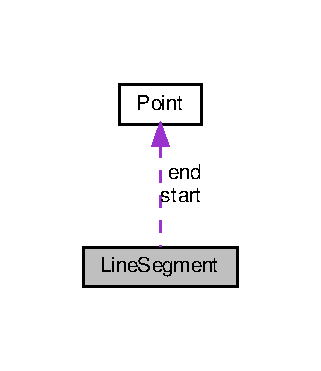
\includegraphics[width=154pt]{class_line_segment__coll__graph}
\end{center}
\end{figure}
\subsection*{Public Member Functions}
\begin{DoxyCompactItemize}
\item 
\hyperlink{class_line_segment_ad006d80e0d72c31734ff22d6c9dfed3d}{Line\+Segment} (\hyperlink{class_point}{Point} x, \hyperlink{class_point}{Point} y)
\begin{DoxyCompactList}\small\item\em \hyperlink{class_line_segment}{Line\+Segment} Default Constructor, a line between 2 points. \end{DoxyCompactList}\item 
\hyperlink{class_point}{Point} \hyperlink{class_line_segment_afcff6bd5f6a3073a44f7b21db0be876f}{get\+Start} () const
\begin{DoxyCompactList}\small\item\em get\+Start getter method for starting point \end{DoxyCompactList}\item 
\hyperlink{class_point}{Point} \hyperlink{class_line_segment_a7b05f883c369b950e61009edfafbbd0e}{get\+End} () const
\begin{DoxyCompactList}\small\item\em get\+End getter method for end of line segment \end{DoxyCompactList}\end{DoxyCompactItemize}
\subsection*{Public Attributes}
\begin{DoxyCompactItemize}
\item 
\hyperlink{class_point}{Point} \hyperlink{class_line_segment_a91bddd96ae050a8255e3180c50f071f5}{start}
\item 
\hyperlink{class_point}{Point} \hyperlink{class_line_segment_acf33c308064ab9c60f47c11b5d23db06}{end}
\end{DoxyCompactItemize}


\subsection{Detailed Description}


Definition at line 112 of file Intersect\+Tester.\+h.



\subsection{Constructor \& Destructor Documentation}
\mbox{\Hypertarget{class_line_segment_ad006d80e0d72c31734ff22d6c9dfed3d}\label{class_line_segment_ad006d80e0d72c31734ff22d6c9dfed3d}} 
\index{Line\+Segment@{Line\+Segment}!Line\+Segment@{Line\+Segment}}
\index{Line\+Segment@{Line\+Segment}!Line\+Segment@{Line\+Segment}}
\subsubsection{\texorpdfstring{Line\+Segment()}{LineSegment()}}
{\footnotesize\ttfamily Line\+Segment\+::\+Line\+Segment (\begin{DoxyParamCaption}\item[{\hyperlink{class_point}{Point}}]{x,  }\item[{\hyperlink{class_point}{Point}}]{y }\end{DoxyParamCaption})\hspace{0.3cm}{\ttfamily [inline]}}



\hyperlink{class_line_segment}{Line\+Segment} Default Constructor, a line between 2 points. 


\begin{DoxyParams}{Parameters}
{\em x} & starting point \\
\hline
{\em y} & ending point \\
\hline
\end{DoxyParams}


Definition at line 121 of file Intersect\+Tester.\+h.


\begin{DoxyCode}
122         \{
123              \hyperlink{class_line_segment_a91bddd96ae050a8255e3180c50f071f5}{start} = \hyperlink{class_point}{Point}(x.\hyperlink{class_point_a29c44ec7c7279e02629645a06cdaf7d5}{getX}(), x.\hyperlink{class_point_a2371ffadbe245d12a8f556d0a976521b}{getY}(), x.\hyperlink{class_point_a9bb9987e32b7dd8dec81ead5d428446c}{getZ}());
124              \hyperlink{class_line_segment_acf33c308064ab9c60f47c11b5d23db06}{end} = \hyperlink{class_point}{Point}(y.\hyperlink{class_point_a29c44ec7c7279e02629645a06cdaf7d5}{getX}(), y.\hyperlink{class_point_a2371ffadbe245d12a8f556d0a976521b}{getY}(), y.\hyperlink{class_point_a9bb9987e32b7dd8dec81ead5d428446c}{getZ}());
125         \}
\end{DoxyCode}


\subsection{Member Function Documentation}
\mbox{\Hypertarget{class_line_segment_a7b05f883c369b950e61009edfafbbd0e}\label{class_line_segment_a7b05f883c369b950e61009edfafbbd0e}} 
\index{Line\+Segment@{Line\+Segment}!get\+End@{get\+End}}
\index{get\+End@{get\+End}!Line\+Segment@{Line\+Segment}}
\subsubsection{\texorpdfstring{get\+End()}{getEnd()}}
{\footnotesize\ttfamily \hyperlink{class_point}{Point} Line\+Segment\+::get\+End (\begin{DoxyParamCaption}{ }\end{DoxyParamCaption}) const\hspace{0.3cm}{\ttfamily [inline]}}



get\+End getter method for end of line segment 

\begin{DoxyReturn}{Returns}
end point of line segment 
\end{DoxyReturn}


Definition at line 135 of file Intersect\+Tester.\+h.


\begin{DoxyCode}
135 \{ \textcolor{keywordflow}{return} \hyperlink{class_line_segment_acf33c308064ab9c60f47c11b5d23db06}{end}; \} 
\end{DoxyCode}
\mbox{\Hypertarget{class_line_segment_afcff6bd5f6a3073a44f7b21db0be876f}\label{class_line_segment_afcff6bd5f6a3073a44f7b21db0be876f}} 
\index{Line\+Segment@{Line\+Segment}!get\+Start@{get\+Start}}
\index{get\+Start@{get\+Start}!Line\+Segment@{Line\+Segment}}
\subsubsection{\texorpdfstring{get\+Start()}{getStart()}}
{\footnotesize\ttfamily \hyperlink{class_point}{Point} Line\+Segment\+::get\+Start (\begin{DoxyParamCaption}{ }\end{DoxyParamCaption}) const\hspace{0.3cm}{\ttfamily [inline]}}



get\+Start getter method for starting point 

\begin{DoxyReturn}{Returns}
starting point of line segment 
\end{DoxyReturn}


Definition at line 130 of file Intersect\+Tester.\+h.


\begin{DoxyCode}
130 \{ \textcolor{keywordflow}{return} \hyperlink{class_line_segment_a91bddd96ae050a8255e3180c50f071f5}{start}; \}
\end{DoxyCode}


\subsection{Member Data Documentation}
\mbox{\Hypertarget{class_line_segment_acf33c308064ab9c60f47c11b5d23db06}\label{class_line_segment_acf33c308064ab9c60f47c11b5d23db06}} 
\index{Line\+Segment@{Line\+Segment}!end@{end}}
\index{end@{end}!Line\+Segment@{Line\+Segment}}
\subsubsection{\texorpdfstring{end}{end}}
{\footnotesize\ttfamily \hyperlink{class_point}{Point} Line\+Segment\+::end}



Definition at line 115 of file Intersect\+Tester.\+h.

\mbox{\Hypertarget{class_line_segment_a91bddd96ae050a8255e3180c50f071f5}\label{class_line_segment_a91bddd96ae050a8255e3180c50f071f5}} 
\index{Line\+Segment@{Line\+Segment}!start@{start}}
\index{start@{start}!Line\+Segment@{Line\+Segment}}
\subsubsection{\texorpdfstring{start}{start}}
{\footnotesize\ttfamily \hyperlink{class_point}{Point} Line\+Segment\+::start}



Definition at line 114 of file Intersect\+Tester.\+h.



The documentation for this class was generated from the following file\+:\begin{DoxyCompactItemize}
\item 
/home/liam/\+Projects/\+Intersection\+Tester\+G\+U\+I/\+Intersect\+Tester/\hyperlink{_intersect_tester_8h}{Intersect\+Tester.\+h}\end{DoxyCompactItemize}

\hypertarget{class_main_interface_window}{}\section{Main\+Interface\+Window Class Reference}
\label{class_main_interface_window}\index{Main\+Interface\+Window@{Main\+Interface\+Window}}


{\ttfamily \#include $<$maininterfacewindow.\+h$>$}



Inheritance diagram for Main\+Interface\+Window\+:
\nopagebreak
\begin{figure}[H]
\begin{center}
\leavevmode
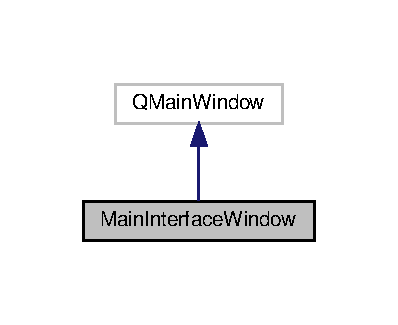
\includegraphics[width=191pt]{class_main_interface_window__inherit__graph}
\end{center}
\end{figure}


Collaboration diagram for Main\+Interface\+Window\+:
\nopagebreak
\begin{figure}[H]
\begin{center}
\leavevmode
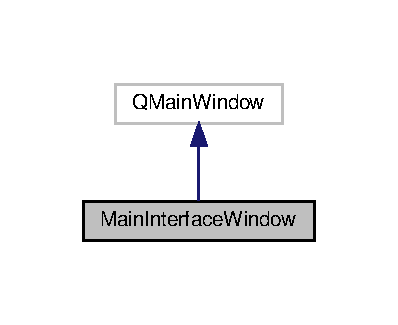
\includegraphics[width=191pt]{class_main_interface_window__coll__graph}
\end{center}
\end{figure}
\subsection*{Public Member Functions}
\begin{DoxyCompactItemize}
\item 
\hyperlink{class_main_interface_window_a8b5aa367c51aca1da2c4e54ddf1571c1}{Main\+Interface\+Window} (Q\+Widget $\ast$parent=0)
\begin{DoxyCompactList}\small\item\em \hyperlink{class_main_interface_window}{Main\+Interface\+Window} constructor. \end{DoxyCompactList}\item 
\hyperlink{class_main_interface_window_a774d48e98f706047f8f12f5f961450d3}{$\sim$\+Main\+Interface\+Window} ()
\end{DoxyCompactItemize}
\subsection*{Private Slots}
\begin{DoxyCompactItemize}
\item 
void \hyperlink{class_main_interface_window_a380d5adfd4f2f434a4dbceba61a3223f}{on\+\_\+cmb\+Static\+\_\+current\+Index\+Changed} ()
\begin{DoxyCompactList}\small\item\em on\+\_\+cmb\+Static\+\_\+current\+Index\+Changed action to switch the state for the static primitive \end{DoxyCompactList}\item 
void \hyperlink{class_main_interface_window_a88d3fa446248d7d4c054cdf9e228571c}{on\+\_\+cmb\+Move\+\_\+current\+Index\+Changed} ()
\begin{DoxyCompactList}\small\item\em on\+\_\+cmb\+Move\+\_\+current\+Index\+Changed action to switch the state for the moving primitive \end{DoxyCompactList}\end{DoxyCompactItemize}
\subsection*{Private Attributes}
\begin{DoxyCompactItemize}
\item 
Ui\+::\+Main\+Interface\+Window $\ast$ \hyperlink{class_main_interface_window_afe3aae95d697ade063b0e4ad517655b9}{ui}
\end{DoxyCompactItemize}


\subsection{Detailed Description}


Definition at line 33 of file maininterfacewindow.\+h.



\subsection{Constructor \& Destructor Documentation}
\mbox{\Hypertarget{class_main_interface_window_a8b5aa367c51aca1da2c4e54ddf1571c1}\label{class_main_interface_window_a8b5aa367c51aca1da2c4e54ddf1571c1}} 
\index{Main\+Interface\+Window@{Main\+Interface\+Window}!Main\+Interface\+Window@{Main\+Interface\+Window}}
\index{Main\+Interface\+Window@{Main\+Interface\+Window}!Main\+Interface\+Window@{Main\+Interface\+Window}}
\subsubsection{\texorpdfstring{Main\+Interface\+Window()}{MainInterfaceWindow()}}
{\footnotesize\ttfamily Main\+Interface\+Window\+::\+Main\+Interface\+Window (\begin{DoxyParamCaption}\item[{Q\+Widget $\ast$}]{parent = {\ttfamily 0} }\end{DoxyParamCaption})\hspace{0.3cm}{\ttfamily [explicit]}}



\hyperlink{class_main_interface_window}{Main\+Interface\+Window} constructor. 


\begin{DoxyParams}{Parameters}
{\em parent} & widget parent \\
\hline
\end{DoxyParams}


Definition at line 4 of file maininterfacewindow.\+cpp.


\begin{DoxyCode}
4                                                         :
5     QMainWindow(parent),
6     \hyperlink{class_main_interface_window_afe3aae95d697ade063b0e4ad517655b9}{ui}(\textcolor{keyword}{new} Ui::MainInterfaceWindow)
7 \{
8     \hyperlink{class_main_interface_window_afe3aae95d697ade063b0e4ad517655b9}{ui}->setupUi(\textcolor{keyword}{this});
9     QStringList list;
10     list << \textcolor{stringliteral}{"Point"} << \textcolor{stringliteral}{"Line"} << \textcolor{stringliteral}{"Circle"} << \textcolor{stringliteral}{"Triangle"} << \textcolor{stringliteral}{"Square"};
11     \hyperlink{class_main_interface_window_afe3aae95d697ade063b0e4ad517655b9}{ui}->cmbMove->addItems(list);
12     \hyperlink{class_main_interface_window_afe3aae95d697ade063b0e4ad517655b9}{ui}->cmbStatic->addItems(list);
13     \hyperlink{class_main_interface_window_afe3aae95d697ade063b0e4ad517655b9}{ui}->cmbStatic->setCurrentIndex(4);
14 \}
\end{DoxyCode}
\mbox{\Hypertarget{class_main_interface_window_a774d48e98f706047f8f12f5f961450d3}\label{class_main_interface_window_a774d48e98f706047f8f12f5f961450d3}} 
\index{Main\+Interface\+Window@{Main\+Interface\+Window}!````~Main\+Interface\+Window@{$\sim$\+Main\+Interface\+Window}}
\index{````~Main\+Interface\+Window@{$\sim$\+Main\+Interface\+Window}!Main\+Interface\+Window@{Main\+Interface\+Window}}
\subsubsection{\texorpdfstring{$\sim$\+Main\+Interface\+Window()}{~MainInterfaceWindow()}}
{\footnotesize\ttfamily Main\+Interface\+Window\+::$\sim$\+Main\+Interface\+Window (\begin{DoxyParamCaption}{ }\end{DoxyParamCaption})}



Definition at line 16 of file maininterfacewindow.\+cpp.


\begin{DoxyCode}
17 \{
18     \textcolor{keyword}{delete} \hyperlink{class_main_interface_window_afe3aae95d697ade063b0e4ad517655b9}{ui};
19 \}
\end{DoxyCode}


\subsection{Member Function Documentation}
\mbox{\Hypertarget{class_main_interface_window_a88d3fa446248d7d4c054cdf9e228571c}\label{class_main_interface_window_a88d3fa446248d7d4c054cdf9e228571c}} 
\index{Main\+Interface\+Window@{Main\+Interface\+Window}!on\+\_\+cmb\+Move\+\_\+current\+Index\+Changed@{on\+\_\+cmb\+Move\+\_\+current\+Index\+Changed}}
\index{on\+\_\+cmb\+Move\+\_\+current\+Index\+Changed@{on\+\_\+cmb\+Move\+\_\+current\+Index\+Changed}!Main\+Interface\+Window@{Main\+Interface\+Window}}
\subsubsection{\texorpdfstring{on\+\_\+cmb\+Move\+\_\+current\+Index\+Changed}{on\_cmbMove\_currentIndexChanged}}
{\footnotesize\ttfamily void Main\+Interface\+Window\+::on\+\_\+cmb\+Move\+\_\+current\+Index\+Changed (\begin{DoxyParamCaption}{ }\end{DoxyParamCaption})\hspace{0.3cm}{\ttfamily [private]}, {\ttfamily [slot]}}



on\+\_\+cmb\+Move\+\_\+current\+Index\+Changed action to switch the state for the moving primitive 



Definition at line 27 of file maininterfacewindow.\+cpp.


\begin{DoxyCode}
28 \{
29     \hyperlink{class_main_interface_window_afe3aae95d697ade063b0e4ad517655b9}{ui}->openGLWidget->setMovingState(\hyperlink{class_main_interface_window_afe3aae95d697ade063b0e4ad517655b9}{ui}->cmbMove->currentIndex());
30     \hyperlink{class_main_interface_window_afe3aae95d697ade063b0e4ad517655b9}{ui}->openGLWidget->update();
31 \}
\end{DoxyCode}
\mbox{\Hypertarget{class_main_interface_window_a380d5adfd4f2f434a4dbceba61a3223f}\label{class_main_interface_window_a380d5adfd4f2f434a4dbceba61a3223f}} 
\index{Main\+Interface\+Window@{Main\+Interface\+Window}!on\+\_\+cmb\+Static\+\_\+current\+Index\+Changed@{on\+\_\+cmb\+Static\+\_\+current\+Index\+Changed}}
\index{on\+\_\+cmb\+Static\+\_\+current\+Index\+Changed@{on\+\_\+cmb\+Static\+\_\+current\+Index\+Changed}!Main\+Interface\+Window@{Main\+Interface\+Window}}
\subsubsection{\texorpdfstring{on\+\_\+cmb\+Static\+\_\+current\+Index\+Changed}{on\_cmbStatic\_currentIndexChanged}}
{\footnotesize\ttfamily void Main\+Interface\+Window\+::on\+\_\+cmb\+Static\+\_\+current\+Index\+Changed (\begin{DoxyParamCaption}{ }\end{DoxyParamCaption})\hspace{0.3cm}{\ttfamily [private]}, {\ttfamily [slot]}}



on\+\_\+cmb\+Static\+\_\+current\+Index\+Changed action to switch the state for the static primitive 



Definition at line 21 of file maininterfacewindow.\+cpp.


\begin{DoxyCode}
22 \{
23     \hyperlink{class_main_interface_window_afe3aae95d697ade063b0e4ad517655b9}{ui}->openGLWidget->setStaticState(\hyperlink{class_main_interface_window_afe3aae95d697ade063b0e4ad517655b9}{ui}->cmbStatic->currentIndex());
24     \hyperlink{class_main_interface_window_afe3aae95d697ade063b0e4ad517655b9}{ui}->openGLWidget->update();
25 \}
\end{DoxyCode}


\subsection{Member Data Documentation}
\mbox{\Hypertarget{class_main_interface_window_afe3aae95d697ade063b0e4ad517655b9}\label{class_main_interface_window_afe3aae95d697ade063b0e4ad517655b9}} 
\index{Main\+Interface\+Window@{Main\+Interface\+Window}!ui@{ui}}
\index{ui@{ui}!Main\+Interface\+Window@{Main\+Interface\+Window}}
\subsubsection{\texorpdfstring{ui}{ui}}
{\footnotesize\ttfamily Ui\+::\+Main\+Interface\+Window$\ast$ Main\+Interface\+Window\+::ui\hspace{0.3cm}{\ttfamily [private]}}



Definition at line 58 of file maininterfacewindow.\+h.



The documentation for this class was generated from the following files\+:\begin{DoxyCompactItemize}
\item 
/home/liam/\+Projects/\+Intersection\+Tester\+G\+U\+I/\hyperlink{maininterfacewindow_8h}{maininterfacewindow.\+h}\item 
/home/liam/\+Projects/\+Intersection\+Tester\+G\+U\+I/\hyperlink{maininterfacewindow_8cpp}{maininterfacewindow.\+cpp}\end{DoxyCompactItemize}

\hypertarget{class_point}{}\section{Point Class Reference}
\label{class_point}\index{Point@{Point}}


{\ttfamily \#include $<$Intersect\+Tester.\+h$>$}

\subsection*{Public Member Functions}
\begin{DoxyCompactItemize}
\item 
\hyperlink{class_point_ad92f2337b839a94ce97dcdb439b4325a}{Point} ()
\begin{DoxyCompactList}\small\item\em \hyperlink{class_point}{Point} Default Constructor. \end{DoxyCompactList}\item 
\hyperlink{class_point_a30bc8409287de4f43e160664be834636}{Point} (float \hyperlink{class_point_a05dfe2dfbde813ad234b514f30e662f1}{x}, float \hyperlink{class_point_a6101960c8d2d4e8ea1d32c9234bbeb8d}{y})
\begin{DoxyCompactList}\small\item\em \hyperlink{class_point}{Point} Constructor for a 2D \hyperlink{class_point}{Point}. \end{DoxyCompactList}\item 
\hyperlink{class_point_a405838cb39b8fb6119633d9ba7e6b4fb}{Point} (float \hyperlink{class_point_a05dfe2dfbde813ad234b514f30e662f1}{x}, float \hyperlink{class_point_a6101960c8d2d4e8ea1d32c9234bbeb8d}{y}, float \hyperlink{class_point_a9a666531e0e99adff132be93d2407d0c}{z})
\begin{DoxyCompactList}\small\item\em \hyperlink{class_point}{Point} Constructor for a 3D \hyperlink{class_point}{Point}. \end{DoxyCompactList}\item 
\hyperlink{class_point}{Point} \& \hyperlink{class_point_a0e75bb40a406c615b5632f36fa035a47}{operator=} (const \hyperlink{class_point}{Point} \&other)
\begin{DoxyCompactList}\small\item\em operator= assignment operator \end{DoxyCompactList}\item 
float \hyperlink{class_point_a29c44ec7c7279e02629645a06cdaf7d5}{getX} () const
\begin{DoxyCompactList}\small\item\em getX getter method for the x axis coordinate reference \end{DoxyCompactList}\item 
float \hyperlink{class_point_a2371ffadbe245d12a8f556d0a976521b}{getY} () const
\begin{DoxyCompactList}\small\item\em getY getter method for the y axis coordinate reference \end{DoxyCompactList}\item 
float \hyperlink{class_point_a9bb9987e32b7dd8dec81ead5d428446c}{getZ} () const
\begin{DoxyCompactList}\small\item\em getZ getter method for the z axis coordinate reference \end{DoxyCompactList}\item 
void \hyperlink{class_point_a337d4410acd500f972f87f4fc73a43fe}{setX} (float newX)
\begin{DoxyCompactList}\small\item\em setX setter method for the x axis coordinate reference \end{DoxyCompactList}\item 
void \hyperlink{class_point_ad77207403cf0e51641b7bc500d351e3f}{setY} (float newY)
\begin{DoxyCompactList}\small\item\em setY setter method for the y axis coordinate reference \end{DoxyCompactList}\item 
void \hyperlink{class_point_a82621ca550dece2b002d8fb5d7b17221}{setZ} (float newZ)
\begin{DoxyCompactList}\small\item\em setZ setter method for the z axis coordinate reference \end{DoxyCompactList}\end{DoxyCompactItemize}
\subsection*{Public Attributes}
\begin{DoxyCompactItemize}
\item 
float \hyperlink{class_point_a05dfe2dfbde813ad234b514f30e662f1}{x}
\item 
float \hyperlink{class_point_a6101960c8d2d4e8ea1d32c9234bbeb8d}{y}
\item 
float \hyperlink{class_point_a9a666531e0e99adff132be93d2407d0c}{z}
\end{DoxyCompactItemize}


\subsection{Detailed Description}
Intersection Tester -\/ v1.\+0.\+0 Original Author\+: Liam Mc\+Nabb Proceeding Author(s)\+: N/A Copyright (c) 2019 Permission is hereby granted, free of charge, to any person obtaining a copy of this software and associated documentation files (Intersection\+Tester), to deal in the Software without restriction, including without limitation the rights to use, copy, modify, merge, publish, distribute, sublicense, and/or sell copies of the Software, and to permit persons to whom the Software is furnished to do so, subject to the following conditions\+: The above copyright notice and this permission notice shall be included in all copies or substantial portions of the Software. T\+HE S\+O\+F\+T\+W\+A\+RE IS P\+R\+O\+V\+I\+D\+ED \char`\"{}\+A\+S I\+S\char`\"{}, W\+I\+T\+H\+O\+UT W\+A\+R\+R\+A\+N\+TY OF A\+NY K\+I\+ND, E\+X\+P\+R\+E\+SS OR I\+M\+P\+L\+I\+ED, I\+N\+C\+L\+U\+D\+I\+NG B\+UT N\+OT L\+I\+M\+I\+T\+ED TO T\+HE W\+A\+R\+R\+A\+N\+T\+I\+ES OF M\+E\+R\+C\+H\+A\+N\+T\+A\+B\+I\+L\+I\+TY, F\+I\+T\+N\+E\+SS F\+OR A P\+A\+R\+T\+I\+C\+U\+L\+AR P\+U\+R\+P\+O\+SE A\+ND N\+O\+N\+I\+N\+F\+R\+I\+N\+G\+E\+M\+E\+NT. IN NO E\+V\+E\+NT S\+H\+A\+LL T\+HE A\+U\+T\+H\+O\+RS OR C\+O\+P\+Y\+R\+I\+G\+HT H\+O\+L\+D\+E\+RS BE L\+I\+A\+B\+LE F\+OR A\+NY C\+L\+A\+IM, D\+A\+M\+A\+G\+ES OR O\+T\+H\+ER L\+I\+A\+B\+I\+L\+I\+TY, W\+H\+E\+T\+H\+ER IN AN A\+C\+T\+I\+ON OF C\+O\+N\+T\+R\+A\+CT, T\+O\+RT OR O\+T\+H\+E\+R\+W\+I\+SE, A\+R\+I\+S\+I\+NG F\+R\+OM, O\+UT OF OR IN C\+O\+N\+N\+E\+C\+T\+I\+ON W\+I\+TH T\+HE S\+O\+F\+T\+W\+A\+RE OR T\+HE U\+SE OR O\+T\+H\+ER D\+E\+A\+L\+I\+N\+GS IN T\+HE S\+O\+F\+T\+W\+A\+RE. 

Definition at line 33 of file Intersect\+Tester.\+h.



\subsection{Constructor \& Destructor Documentation}
\mbox{\Hypertarget{class_point_ad92f2337b839a94ce97dcdb439b4325a}\label{class_point_ad92f2337b839a94ce97dcdb439b4325a}} 
\index{Point@{Point}!Point@{Point}}
\index{Point@{Point}!Point@{Point}}
\subsubsection{\texorpdfstring{Point()}{Point()}\hspace{0.1cm}{\footnotesize\ttfamily [1/3]}}
{\footnotesize\ttfamily Point\+::\+Point (\begin{DoxyParamCaption}{ }\end{DoxyParamCaption})\hspace{0.3cm}{\ttfamily [inline]}}



\hyperlink{class_point}{Point} Default Constructor. 



Definition at line 39 of file Intersect\+Tester.\+h.


\begin{DoxyCode}
40         \{
41             this->\hyperlink{class_point_a05dfe2dfbde813ad234b514f30e662f1}{x} = 0;
42             this->\hyperlink{class_point_a6101960c8d2d4e8ea1d32c9234bbeb8d}{y} = 0;
43             this->\hyperlink{class_point_a9a666531e0e99adff132be93d2407d0c}{z} = 0;
44         \}
\end{DoxyCode}
\mbox{\Hypertarget{class_point_a30bc8409287de4f43e160664be834636}\label{class_point_a30bc8409287de4f43e160664be834636}} 
\index{Point@{Point}!Point@{Point}}
\index{Point@{Point}!Point@{Point}}
\subsubsection{\texorpdfstring{Point()}{Point()}\hspace{0.1cm}{\footnotesize\ttfamily [2/3]}}
{\footnotesize\ttfamily Point\+::\+Point (\begin{DoxyParamCaption}\item[{float}]{x,  }\item[{float}]{y }\end{DoxyParamCaption})\hspace{0.3cm}{\ttfamily [inline]}}



\hyperlink{class_point}{Point} Constructor for a 2D \hyperlink{class_point}{Point}. 


\begin{DoxyParams}{Parameters}
{\em x} & \\
\hline
{\em y} & \\
\hline
\end{DoxyParams}


Definition at line 50 of file Intersect\+Tester.\+h.


\begin{DoxyCode}
51         \{
52             this->\hyperlink{class_point_a05dfe2dfbde813ad234b514f30e662f1}{x} = \hyperlink{class_point_a05dfe2dfbde813ad234b514f30e662f1}{x};
53             this->\hyperlink{class_point_a6101960c8d2d4e8ea1d32c9234bbeb8d}{y} = \hyperlink{class_point_a6101960c8d2d4e8ea1d32c9234bbeb8d}{y};
54             this->\hyperlink{class_point_a9a666531e0e99adff132be93d2407d0c}{z} = 0;
55         \}
\end{DoxyCode}
\mbox{\Hypertarget{class_point_a405838cb39b8fb6119633d9ba7e6b4fb}\label{class_point_a405838cb39b8fb6119633d9ba7e6b4fb}} 
\index{Point@{Point}!Point@{Point}}
\index{Point@{Point}!Point@{Point}}
\subsubsection{\texorpdfstring{Point()}{Point()}\hspace{0.1cm}{\footnotesize\ttfamily [3/3]}}
{\footnotesize\ttfamily Point\+::\+Point (\begin{DoxyParamCaption}\item[{float}]{x,  }\item[{float}]{y,  }\item[{float}]{z }\end{DoxyParamCaption})\hspace{0.3cm}{\ttfamily [inline]}}



\hyperlink{class_point}{Point} Constructor for a 3D \hyperlink{class_point}{Point}. 


\begin{DoxyParams}{Parameters}
{\em x} & \\
\hline
{\em y} & \\
\hline
{\em z} & \\
\hline
\end{DoxyParams}


Definition at line 62 of file Intersect\+Tester.\+h.


\begin{DoxyCode}
63         \{
64             this->\hyperlink{class_point_a05dfe2dfbde813ad234b514f30e662f1}{x} = \hyperlink{class_point_a05dfe2dfbde813ad234b514f30e662f1}{x};
65             this->\hyperlink{class_point_a6101960c8d2d4e8ea1d32c9234bbeb8d}{y} = \hyperlink{class_point_a6101960c8d2d4e8ea1d32c9234bbeb8d}{y};
66             this->\hyperlink{class_point_a9a666531e0e99adff132be93d2407d0c}{z} = \hyperlink{class_point_a9a666531e0e99adff132be93d2407d0c}{z};
67         \}
\end{DoxyCode}


\subsection{Member Function Documentation}
\mbox{\Hypertarget{class_point_a29c44ec7c7279e02629645a06cdaf7d5}\label{class_point_a29c44ec7c7279e02629645a06cdaf7d5}} 
\index{Point@{Point}!getX@{getX}}
\index{getX@{getX}!Point@{Point}}
\subsubsection{\texorpdfstring{get\+X()}{getX()}}
{\footnotesize\ttfamily float Point\+::getX (\begin{DoxyParamCaption}{ }\end{DoxyParamCaption}) const\hspace{0.3cm}{\ttfamily [inline]}}



getX getter method for the x axis coordinate reference 

\begin{DoxyReturn}{Returns}
float depicting x axis coordinate reference 
\end{DoxyReturn}


Definition at line 84 of file Intersect\+Tester.\+h.


\begin{DoxyCode}
84 \{ \textcolor{keywordflow}{return} \hyperlink{class_point_a05dfe2dfbde813ad234b514f30e662f1}{x}; \}
\end{DoxyCode}
\mbox{\Hypertarget{class_point_a2371ffadbe245d12a8f556d0a976521b}\label{class_point_a2371ffadbe245d12a8f556d0a976521b}} 
\index{Point@{Point}!getY@{getY}}
\index{getY@{getY}!Point@{Point}}
\subsubsection{\texorpdfstring{get\+Y()}{getY()}}
{\footnotesize\ttfamily float Point\+::getY (\begin{DoxyParamCaption}{ }\end{DoxyParamCaption}) const\hspace{0.3cm}{\ttfamily [inline]}}



getY getter method for the y axis coordinate reference 

\begin{DoxyReturn}{Returns}
float depicting y axis coordinate reference 
\end{DoxyReturn}


Definition at line 89 of file Intersect\+Tester.\+h.


\begin{DoxyCode}
89 \{ \textcolor{keywordflow}{return} \hyperlink{class_point_a6101960c8d2d4e8ea1d32c9234bbeb8d}{y}; \}
\end{DoxyCode}
\mbox{\Hypertarget{class_point_a9bb9987e32b7dd8dec81ead5d428446c}\label{class_point_a9bb9987e32b7dd8dec81ead5d428446c}} 
\index{Point@{Point}!getZ@{getZ}}
\index{getZ@{getZ}!Point@{Point}}
\subsubsection{\texorpdfstring{get\+Z()}{getZ()}}
{\footnotesize\ttfamily float Point\+::getZ (\begin{DoxyParamCaption}{ }\end{DoxyParamCaption}) const\hspace{0.3cm}{\ttfamily [inline]}}



getZ getter method for the z axis coordinate reference 

\begin{DoxyReturn}{Returns}
float depicting z axis coordinate reference 
\end{DoxyReturn}


Definition at line 94 of file Intersect\+Tester.\+h.


\begin{DoxyCode}
94 \{ \textcolor{keywordflow}{return} \hyperlink{class_point_a9a666531e0e99adff132be93d2407d0c}{z}; \}
\end{DoxyCode}
\mbox{\Hypertarget{class_point_a0e75bb40a406c615b5632f36fa035a47}\label{class_point_a0e75bb40a406c615b5632f36fa035a47}} 
\index{Point@{Point}!operator=@{operator=}}
\index{operator=@{operator=}!Point@{Point}}
\subsubsection{\texorpdfstring{operator=()}{operator=()}}
{\footnotesize\ttfamily \hyperlink{class_point}{Point}\& Point\+::operator= (\begin{DoxyParamCaption}\item[{const \hyperlink{class_point}{Point} \&}]{other }\end{DoxyParamCaption})\hspace{0.3cm}{\ttfamily [inline]}}



operator= assignment operator 


\begin{DoxyParams}{Parameters}
{\em other} & the point to assign to this object \\
\hline
\end{DoxyParams}
\begin{DoxyReturn}{Returns}
return this object 
\end{DoxyReturn}


Definition at line 73 of file Intersect\+Tester.\+h.


\begin{DoxyCode}
74          \{
75              \hyperlink{class_point_a05dfe2dfbde813ad234b514f30e662f1}{x} = other.\hyperlink{class_point_a29c44ec7c7279e02629645a06cdaf7d5}{getX}();
76              \hyperlink{class_point_a6101960c8d2d4e8ea1d32c9234bbeb8d}{y} = other.\hyperlink{class_point_a2371ffadbe245d12a8f556d0a976521b}{getY}();
77              \hyperlink{class_point_a9a666531e0e99adff132be93d2407d0c}{z} = other.\hyperlink{class_point_a9bb9987e32b7dd8dec81ead5d428446c}{getZ}();
78              \textcolor{keywordflow}{return} *\textcolor{keyword}{this};
79          \}
\end{DoxyCode}
\mbox{\Hypertarget{class_point_a337d4410acd500f972f87f4fc73a43fe}\label{class_point_a337d4410acd500f972f87f4fc73a43fe}} 
\index{Point@{Point}!setX@{setX}}
\index{setX@{setX}!Point@{Point}}
\subsubsection{\texorpdfstring{set\+X()}{setX()}}
{\footnotesize\ttfamily void Point\+::setX (\begin{DoxyParamCaption}\item[{float}]{newX }\end{DoxyParamCaption})\hspace{0.3cm}{\ttfamily [inline]}}



setX setter method for the x axis coordinate reference 


\begin{DoxyParams}{Parameters}
{\em newX} & new value for the x axis coordinate reference \\
\hline
\end{DoxyParams}


Definition at line 99 of file Intersect\+Tester.\+h.


\begin{DoxyCode}
99 \{ \hyperlink{class_point_a05dfe2dfbde813ad234b514f30e662f1}{x} = newX; \}
\end{DoxyCode}
\mbox{\Hypertarget{class_point_ad77207403cf0e51641b7bc500d351e3f}\label{class_point_ad77207403cf0e51641b7bc500d351e3f}} 
\index{Point@{Point}!setY@{setY}}
\index{setY@{setY}!Point@{Point}}
\subsubsection{\texorpdfstring{set\+Y()}{setY()}}
{\footnotesize\ttfamily void Point\+::setY (\begin{DoxyParamCaption}\item[{float}]{newY }\end{DoxyParamCaption})\hspace{0.3cm}{\ttfamily [inline]}}



setY setter method for the y axis coordinate reference 


\begin{DoxyParams}{Parameters}
{\em newY} & new value for the y axis coordinate reference \\
\hline
\end{DoxyParams}


Definition at line 104 of file Intersect\+Tester.\+h.


\begin{DoxyCode}
104 \{ \hyperlink{class_point_a6101960c8d2d4e8ea1d32c9234bbeb8d}{y} = newY; \}
\end{DoxyCode}
\mbox{\Hypertarget{class_point_a82621ca550dece2b002d8fb5d7b17221}\label{class_point_a82621ca550dece2b002d8fb5d7b17221}} 
\index{Point@{Point}!setZ@{setZ}}
\index{setZ@{setZ}!Point@{Point}}
\subsubsection{\texorpdfstring{set\+Z()}{setZ()}}
{\footnotesize\ttfamily void Point\+::setZ (\begin{DoxyParamCaption}\item[{float}]{newZ }\end{DoxyParamCaption})\hspace{0.3cm}{\ttfamily [inline]}}



setZ setter method for the z axis coordinate reference 


\begin{DoxyParams}{Parameters}
{\em newZ} & new value for the z axis coordinate reference \\
\hline
\end{DoxyParams}


Definition at line 109 of file Intersect\+Tester.\+h.


\begin{DoxyCode}
109 \{ \hyperlink{class_point_a9a666531e0e99adff132be93d2407d0c}{z} = newZ; \}
\end{DoxyCode}


\subsection{Member Data Documentation}
\mbox{\Hypertarget{class_point_a05dfe2dfbde813ad234b514f30e662f1}\label{class_point_a05dfe2dfbde813ad234b514f30e662f1}} 
\index{Point@{Point}!x@{x}}
\index{x@{x}!Point@{Point}}
\subsubsection{\texorpdfstring{x}{x}}
{\footnotesize\ttfamily float Point\+::x}



Definition at line 35 of file Intersect\+Tester.\+h.

\mbox{\Hypertarget{class_point_a6101960c8d2d4e8ea1d32c9234bbeb8d}\label{class_point_a6101960c8d2d4e8ea1d32c9234bbeb8d}} 
\index{Point@{Point}!y@{y}}
\index{y@{y}!Point@{Point}}
\subsubsection{\texorpdfstring{y}{y}}
{\footnotesize\ttfamily float Point\+::y}



Definition at line 35 of file Intersect\+Tester.\+h.

\mbox{\Hypertarget{class_point_a9a666531e0e99adff132be93d2407d0c}\label{class_point_a9a666531e0e99adff132be93d2407d0c}} 
\index{Point@{Point}!z@{z}}
\index{z@{z}!Point@{Point}}
\subsubsection{\texorpdfstring{z}{z}}
{\footnotesize\ttfamily float Point\+::z}



Definition at line 35 of file Intersect\+Tester.\+h.



The documentation for this class was generated from the following file\+:\begin{DoxyCompactItemize}
\item 
/home/liam/\+Projects/\+Intersection\+Tester\+G\+U\+I/\+Intersect\+Tester/\hyperlink{_intersect_tester_8h}{Intersect\+Tester.\+h}\end{DoxyCompactItemize}

\hypertarget{class_triangle}{}\section{Triangle Class Reference}
\label{class_triangle}\index{Triangle@{Triangle}}


{\ttfamily \#include $<$Intersect\+Tester.\+h$>$}



Collaboration diagram for Triangle\+:\nopagebreak
\begin{figure}[H]
\begin{center}
\leavevmode
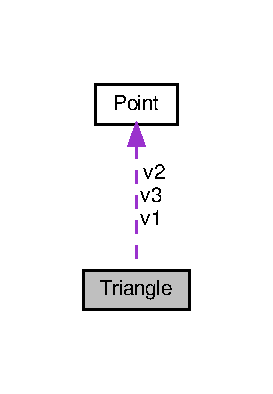
\includegraphics[width=131pt]{class_triangle__coll__graph}
\end{center}
\end{figure}
\subsection*{Public Member Functions}
\begin{DoxyCompactItemize}
\item 
\hyperlink{class_triangle_a07f457e0c5ff143c4cabb39174859a1e}{Triangle} (\hyperlink{class_point}{Point} x, \hyperlink{class_point}{Point} y, \hyperlink{class_point}{Point} z)
\begin{DoxyCompactList}\small\item\em \hyperlink{class_triangle}{Triangle} Default consructor for triangle. \end{DoxyCompactList}\item 
\hyperlink{class_point}{Point} \hyperlink{class_triangle_a88a35d0b66c9636a9be88adc88d003aa}{get\+Vertex\+One} () const
\begin{DoxyCompactList}\small\item\em get\+Vertex\+One getter method for the first vertex \end{DoxyCompactList}\item 
\hyperlink{class_point}{Point} \hyperlink{class_triangle_ac1ae7463f829bcf377fd926b1ad10cac}{get\+Vertex\+Two} () const
\begin{DoxyCompactList}\small\item\em get\+Vertex\+Two getter method for the second vertex \end{DoxyCompactList}\item 
\hyperlink{class_point}{Point} \hyperlink{class_triangle_aed6ceca804b35da95d3d3c930de41e91}{get\+Vertex\+Three} () const
\begin{DoxyCompactList}\small\item\em get\+Vertex\+Three getter method for the third vertex \end{DoxyCompactList}\end{DoxyCompactItemize}
\subsection*{Public Attributes}
\begin{DoxyCompactItemize}
\item 
\hyperlink{class_point}{Point} \hyperlink{class_triangle_a64531c5c908b4ba8aca8b619b97a17bc}{v1}
\item 
\hyperlink{class_point}{Point} \hyperlink{class_triangle_a23721a1b58e5e427c1ac65e311e2828d}{v2}
\item 
\hyperlink{class_point}{Point} \hyperlink{class_triangle_a9ffab42f55ebdbaa549cb1cc592b1c76}{v3}
\end{DoxyCompactItemize}


\subsection{Detailed Description}


Definition at line 139 of file Intersect\+Tester.\+h.



\subsection{Constructor \& Destructor Documentation}
\mbox{\Hypertarget{class_triangle_a07f457e0c5ff143c4cabb39174859a1e}\label{class_triangle_a07f457e0c5ff143c4cabb39174859a1e}} 
\index{Triangle@{Triangle}!Triangle@{Triangle}}
\index{Triangle@{Triangle}!Triangle@{Triangle}}
\subsubsection{\texorpdfstring{Triangle()}{Triangle()}}
{\footnotesize\ttfamily Triangle\+::\+Triangle (\begin{DoxyParamCaption}\item[{\hyperlink{class_point}{Point}}]{x,  }\item[{\hyperlink{class_point}{Point}}]{y,  }\item[{\hyperlink{class_point}{Point}}]{z }\end{DoxyParamCaption})\hspace{0.3cm}{\ttfamily [inline]}}



\hyperlink{class_triangle}{Triangle} Default consructor for triangle. 


\begin{DoxyParams}{Parameters}
{\em x} & vertex one \\
\hline
{\em y} & vertex two \\
\hline
{\em z} & vertex three \\
\hline
\end{DoxyParams}


Definition at line 148 of file Intersect\+Tester.\+h.


\begin{DoxyCode}
149         \{
150              \hyperlink{class_triangle_a64531c5c908b4ba8aca8b619b97a17bc}{v1} = \hyperlink{class_point}{Point}(x.\hyperlink{class_point_a29c44ec7c7279e02629645a06cdaf7d5}{getX}(), x.\hyperlink{class_point_a2371ffadbe245d12a8f556d0a976521b}{getY}(), x.\hyperlink{class_point_a9bb9987e32b7dd8dec81ead5d428446c}{getZ}());
151              \hyperlink{class_triangle_a23721a1b58e5e427c1ac65e311e2828d}{v2} = \hyperlink{class_point}{Point}(y.\hyperlink{class_point_a29c44ec7c7279e02629645a06cdaf7d5}{getX}(), y.\hyperlink{class_point_a2371ffadbe245d12a8f556d0a976521b}{getY}(), y.\hyperlink{class_point_a9bb9987e32b7dd8dec81ead5d428446c}{getZ}());
152              \hyperlink{class_triangle_a9ffab42f55ebdbaa549cb1cc592b1c76}{v3} = \hyperlink{class_point}{Point}(z.\hyperlink{class_point_a29c44ec7c7279e02629645a06cdaf7d5}{getX}(), z.\hyperlink{class_point_a2371ffadbe245d12a8f556d0a976521b}{getY}(), z.\hyperlink{class_point_a9bb9987e32b7dd8dec81ead5d428446c}{getZ}());
153         \}
\end{DoxyCode}


\subsection{Member Function Documentation}
\mbox{\Hypertarget{class_triangle_a88a35d0b66c9636a9be88adc88d003aa}\label{class_triangle_a88a35d0b66c9636a9be88adc88d003aa}} 
\index{Triangle@{Triangle}!get\+Vertex\+One@{get\+Vertex\+One}}
\index{get\+Vertex\+One@{get\+Vertex\+One}!Triangle@{Triangle}}
\subsubsection{\texorpdfstring{get\+Vertex\+One()}{getVertexOne()}}
{\footnotesize\ttfamily \hyperlink{class_point}{Point} Triangle\+::get\+Vertex\+One (\begin{DoxyParamCaption}{ }\end{DoxyParamCaption}) const\hspace{0.3cm}{\ttfamily [inline]}}



get\+Vertex\+One getter method for the first vertex 

\begin{DoxyReturn}{Returns}
vertex one 
\end{DoxyReturn}


Definition at line 158 of file Intersect\+Tester.\+h.


\begin{DoxyCode}
158 \{ \textcolor{keywordflow}{return} \hyperlink{class_triangle_a64531c5c908b4ba8aca8b619b97a17bc}{v1}; \} 
\end{DoxyCode}
\mbox{\Hypertarget{class_triangle_aed6ceca804b35da95d3d3c930de41e91}\label{class_triangle_aed6ceca804b35da95d3d3c930de41e91}} 
\index{Triangle@{Triangle}!get\+Vertex\+Three@{get\+Vertex\+Three}}
\index{get\+Vertex\+Three@{get\+Vertex\+Three}!Triangle@{Triangle}}
\subsubsection{\texorpdfstring{get\+Vertex\+Three()}{getVertexThree()}}
{\footnotesize\ttfamily \hyperlink{class_point}{Point} Triangle\+::get\+Vertex\+Three (\begin{DoxyParamCaption}{ }\end{DoxyParamCaption}) const\hspace{0.3cm}{\ttfamily [inline]}}



get\+Vertex\+Three getter method for the third vertex 

\begin{DoxyReturn}{Returns}
vertex three 
\end{DoxyReturn}


Definition at line 168 of file Intersect\+Tester.\+h.


\begin{DoxyCode}
168 \{ \textcolor{keywordflow}{return} \hyperlink{class_triangle_a9ffab42f55ebdbaa549cb1cc592b1c76}{v3}; \} 
\end{DoxyCode}
\mbox{\Hypertarget{class_triangle_ac1ae7463f829bcf377fd926b1ad10cac}\label{class_triangle_ac1ae7463f829bcf377fd926b1ad10cac}} 
\index{Triangle@{Triangle}!get\+Vertex\+Two@{get\+Vertex\+Two}}
\index{get\+Vertex\+Two@{get\+Vertex\+Two}!Triangle@{Triangle}}
\subsubsection{\texorpdfstring{get\+Vertex\+Two()}{getVertexTwo()}}
{\footnotesize\ttfamily \hyperlink{class_point}{Point} Triangle\+::get\+Vertex\+Two (\begin{DoxyParamCaption}{ }\end{DoxyParamCaption}) const\hspace{0.3cm}{\ttfamily [inline]}}



get\+Vertex\+Two getter method for the second vertex 

\begin{DoxyReturn}{Returns}
vertex two 
\end{DoxyReturn}


Definition at line 163 of file Intersect\+Tester.\+h.


\begin{DoxyCode}
163 \{ \textcolor{keywordflow}{return} \hyperlink{class_triangle_a23721a1b58e5e427c1ac65e311e2828d}{v2}; \} 
\end{DoxyCode}


\subsection{Member Data Documentation}
\mbox{\Hypertarget{class_triangle_a64531c5c908b4ba8aca8b619b97a17bc}\label{class_triangle_a64531c5c908b4ba8aca8b619b97a17bc}} 
\index{Triangle@{Triangle}!v1@{v1}}
\index{v1@{v1}!Triangle@{Triangle}}
\subsubsection{\texorpdfstring{v1}{v1}}
{\footnotesize\ttfamily \hyperlink{class_point}{Point} Triangle\+::v1}



Definition at line 141 of file Intersect\+Tester.\+h.

\mbox{\Hypertarget{class_triangle_a23721a1b58e5e427c1ac65e311e2828d}\label{class_triangle_a23721a1b58e5e427c1ac65e311e2828d}} 
\index{Triangle@{Triangle}!v2@{v2}}
\index{v2@{v2}!Triangle@{Triangle}}
\subsubsection{\texorpdfstring{v2}{v2}}
{\footnotesize\ttfamily \hyperlink{class_point}{Point} Triangle\+::v2}



Definition at line 141 of file Intersect\+Tester.\+h.

\mbox{\Hypertarget{class_triangle_a9ffab42f55ebdbaa549cb1cc592b1c76}\label{class_triangle_a9ffab42f55ebdbaa549cb1cc592b1c76}} 
\index{Triangle@{Triangle}!v3@{v3}}
\index{v3@{v3}!Triangle@{Triangle}}
\subsubsection{\texorpdfstring{v3}{v3}}
{\footnotesize\ttfamily \hyperlink{class_point}{Point} Triangle\+::v3}



Definition at line 141 of file Intersect\+Tester.\+h.



The documentation for this class was generated from the following file\+:\begin{DoxyCompactItemize}
\item 
/home/liam/\+Projects/\+Intersection\+Tester\+G\+U\+I/\+Intersect\+Tester/\hyperlink{_intersect_tester_8h}{Intersect\+Tester.\+h}\end{DoxyCompactItemize}

\chapter{File Documentation}
\hypertarget{canvas_8cpp}{}\section{/home/liam/\+Projects/\+Intersection\+Tester\+G\+U\+I/canvas.cpp File Reference}
\label{canvas_8cpp}\index{/home/liam/\+Projects/\+Intersection\+Tester\+G\+U\+I/canvas.\+cpp@{/home/liam/\+Projects/\+Intersection\+Tester\+G\+U\+I/canvas.\+cpp}}
{\ttfamily \#include \char`\"{}canvas.\+h\char`\"{}}\newline
Include dependency graph for canvas.\+cpp\+:
\nopagebreak
\begin{figure}[H]
\begin{center}
\leavevmode
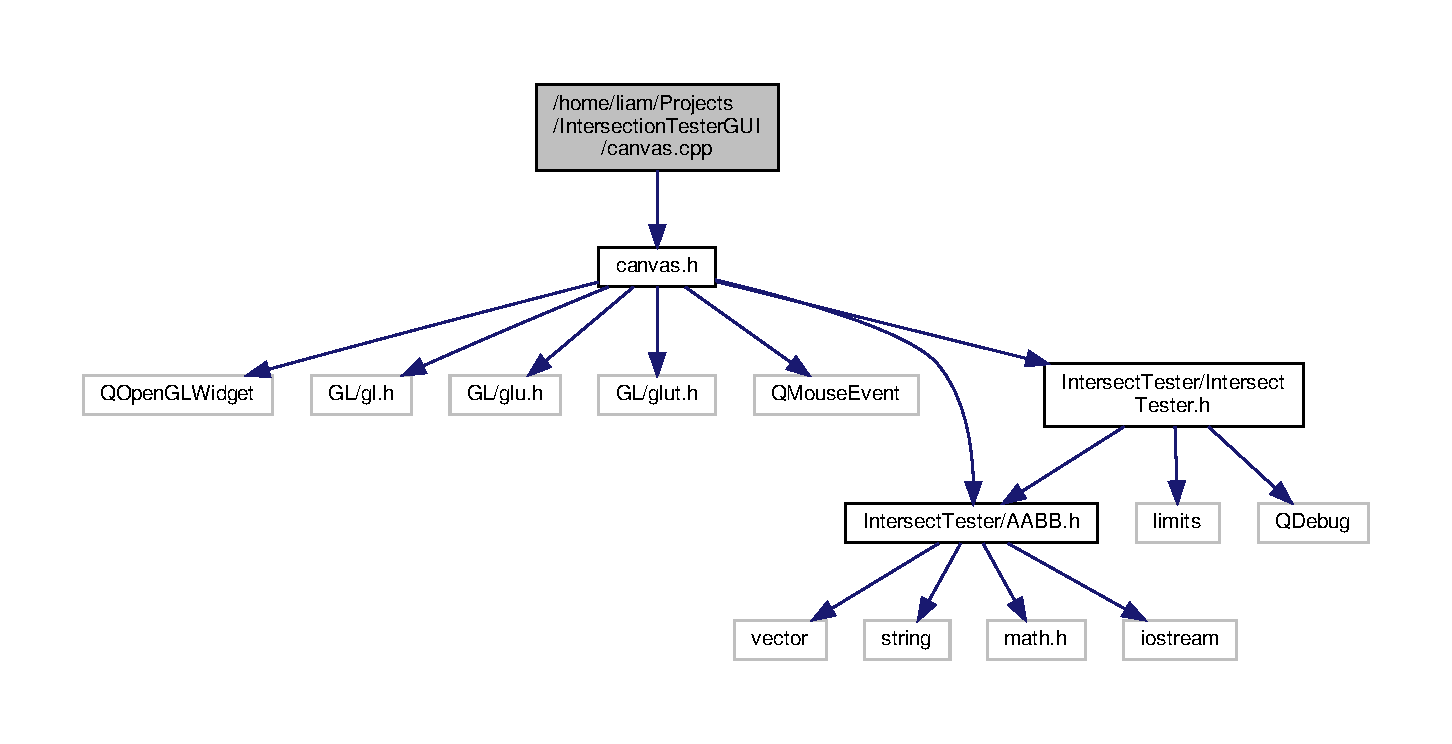
\includegraphics[width=350pt]{canvas_8cpp__incl}
\end{center}
\end{figure}

\hypertarget{canvas_8h}{}\section{/home/liam/\+Projects/\+Intersection\+Tester\+G\+U\+I/canvas.h File Reference}
\label{canvas_8h}\index{/home/liam/\+Projects/\+Intersection\+Tester\+G\+U\+I/canvas.\+h@{/home/liam/\+Projects/\+Intersection\+Tester\+G\+U\+I/canvas.\+h}}
{\ttfamily \#include $<$Q\+Open\+G\+L\+Widget$>$}\newline
{\ttfamily \#include $<$G\+L/gl.\+h$>$}\newline
{\ttfamily \#include $<$G\+L/glu.\+h$>$}\newline
{\ttfamily \#include $<$G\+L/glut.\+h$>$}\newline
{\ttfamily \#include $<$Q\+Mouse\+Event$>$}\newline
{\ttfamily \#include $<$Intersect\+Tester/\+A\+A\+B\+B.\+h$>$}\newline
{\ttfamily \#include $<$Intersect\+Tester/\+Intersect\+Tester.\+h$>$}\newline
Include dependency graph for canvas.\+h\+:
\nopagebreak
\begin{figure}[H]
\begin{center}
\leavevmode
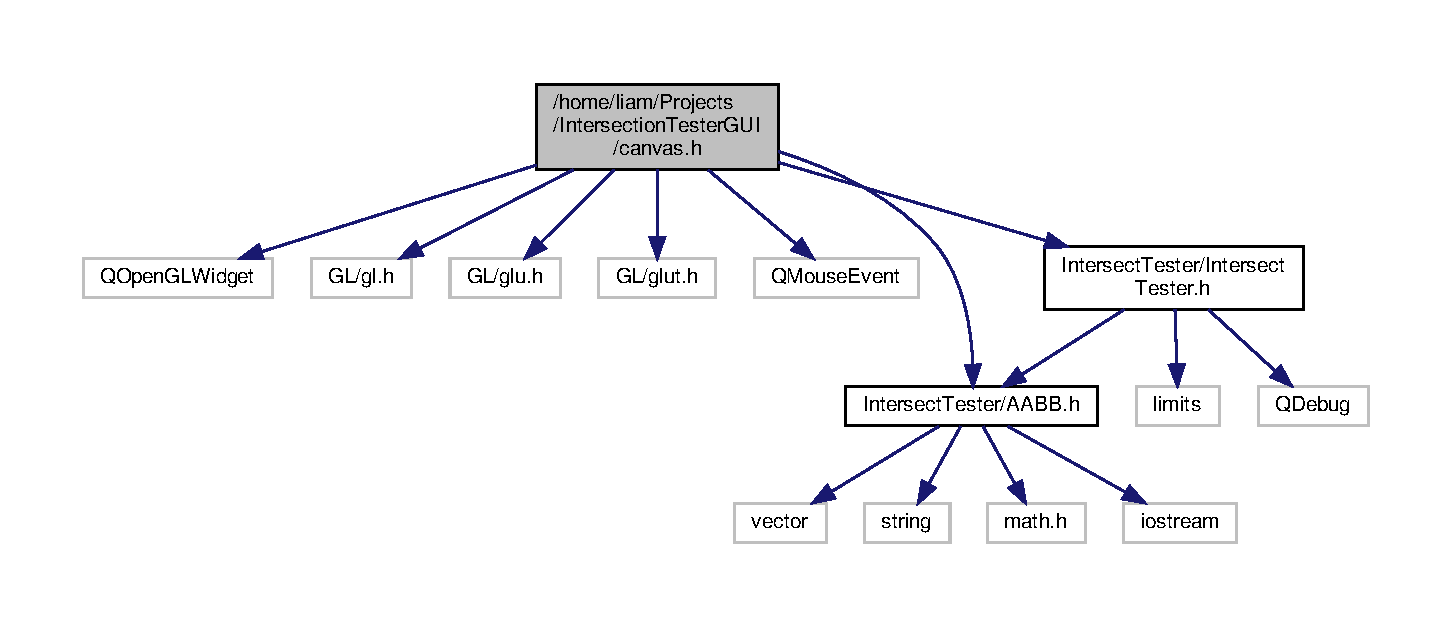
\includegraphics[width=350pt]{canvas_8h__incl}
\end{center}
\end{figure}
This graph shows which files directly or indirectly include this file\+:
\nopagebreak
\begin{figure}[H]
\begin{center}
\leavevmode
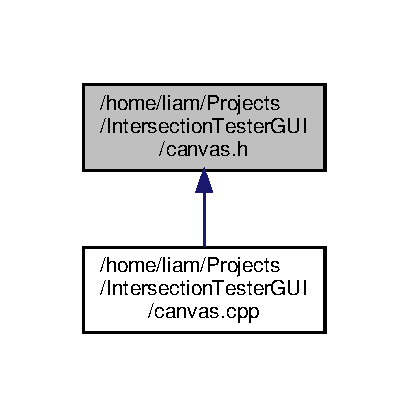
\includegraphics[width=196pt]{canvas_8h__dep__incl}
\end{center}
\end{figure}
\subsection*{Classes}
\begin{DoxyCompactItemize}
\item 
class \hyperlink{class_canvas}{Canvas}
\end{DoxyCompactItemize}

\hypertarget{_a_a_b_b_8cpp}{}\section{/home/liam/\+Projects/\+Intersection\+Tester\+G\+U\+I/\+Intersect\+Tester/\+A\+A\+BB.cpp File Reference}
\label{_a_a_b_b_8cpp}\index{/home/liam/\+Projects/\+Intersection\+Tester\+G\+U\+I/\+Intersect\+Tester/\+A\+A\+B\+B.\+cpp@{/home/liam/\+Projects/\+Intersection\+Tester\+G\+U\+I/\+Intersect\+Tester/\+A\+A\+B\+B.\+cpp}}
{\ttfamily \#include \char`\"{}Intersect\+Tester/\+A\+A\+B\+B.\+h\char`\"{}}\newline
Include dependency graph for A\+A\+B\+B.\+cpp\+:
\nopagebreak
\begin{figure}[H]
\begin{center}
\leavevmode
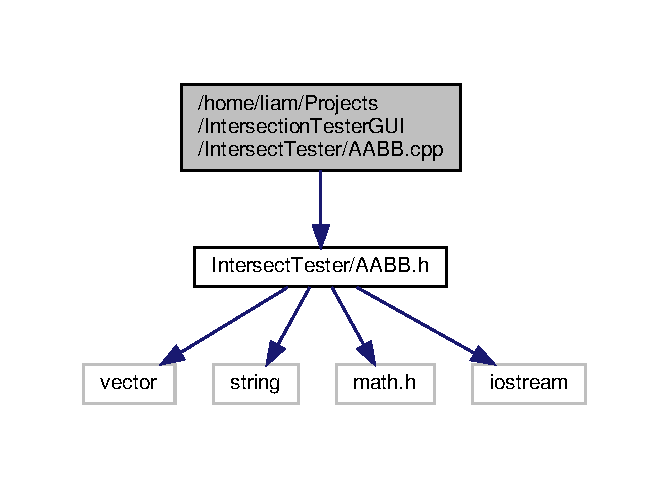
\includegraphics[width=321pt]{_a_a_b_b_8cpp__incl}
\end{center}
\end{figure}

\hypertarget{_a_a_b_b_8h}{}\section{/home/liam/\+Projects/\+Intersection\+Tester\+G\+U\+I/\+Intersect\+Tester/\+A\+A\+BB.h File Reference}
\label{_a_a_b_b_8h}\index{/home/liam/\+Projects/\+Intersection\+Tester\+G\+U\+I/\+Intersect\+Tester/\+A\+A\+B\+B.\+h@{/home/liam/\+Projects/\+Intersection\+Tester\+G\+U\+I/\+Intersect\+Tester/\+A\+A\+B\+B.\+h}}
{\ttfamily \#include $<$vector$>$}\newline
{\ttfamily \#include $<$string$>$}\newline
{\ttfamily \#include $<$math.\+h$>$}\newline
{\ttfamily \#include $<$iostream$>$}\newline
Include dependency graph for A\+A\+B\+B.\+h\+:
\nopagebreak
\begin{figure}[H]
\begin{center}
\leavevmode
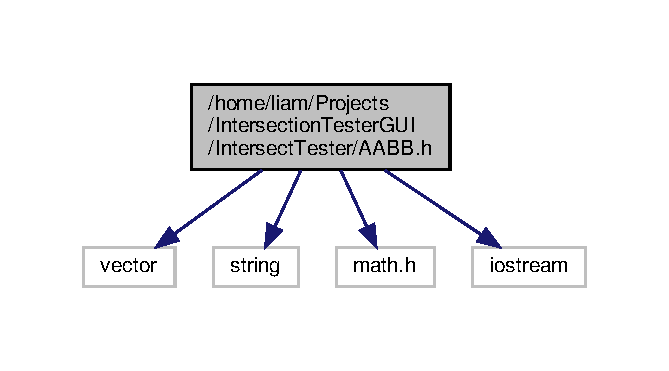
\includegraphics[width=321pt]{_a_a_b_b_8h__incl}
\end{center}
\end{figure}
This graph shows which files directly or indirectly include this file\+:
\nopagebreak
\begin{figure}[H]
\begin{center}
\leavevmode
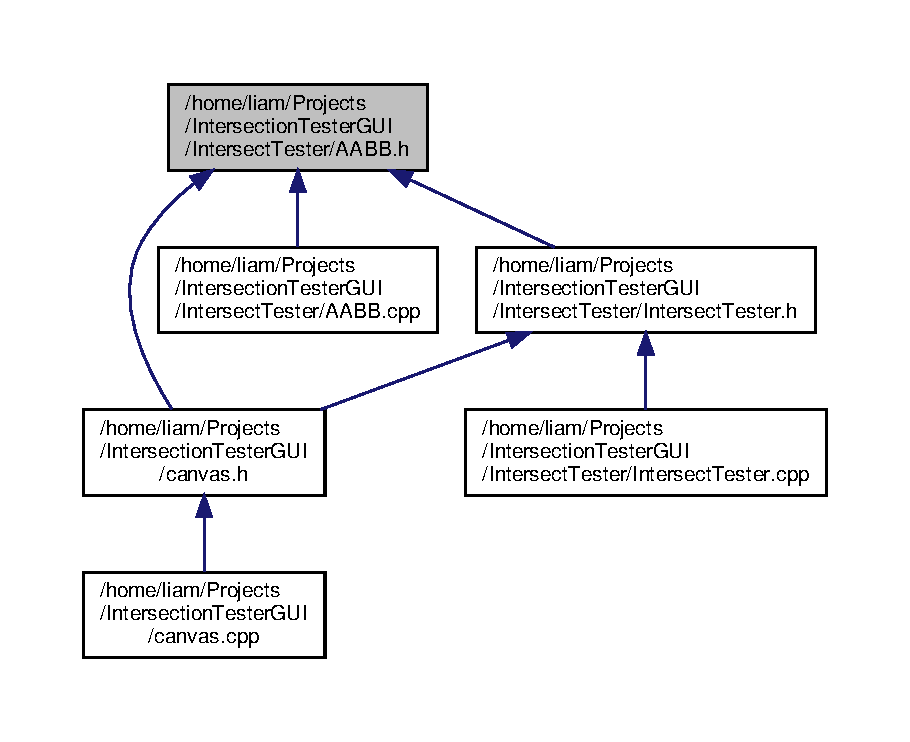
\includegraphics[width=350pt]{_a_a_b_b_8h__dep__incl}
\end{center}
\end{figure}
\subsection*{Classes}
\begin{DoxyCompactItemize}
\item 
class \hyperlink{class_a_a_b_b}{A\+A\+BB}
\end{DoxyCompactItemize}

\hypertarget{_intersect_tester_8cpp}{}\section{/home/liam/\+Projects/\+Intersection\+Tester\+G\+U\+I/\+Intersect\+Tester/\+Intersect\+Tester.cpp File Reference}
\label{_intersect_tester_8cpp}\index{/home/liam/\+Projects/\+Intersection\+Tester\+G\+U\+I/\+Intersect\+Tester/\+Intersect\+Tester.\+cpp@{/home/liam/\+Projects/\+Intersection\+Tester\+G\+U\+I/\+Intersect\+Tester/\+Intersect\+Tester.\+cpp}}
{\ttfamily \#include \char`\"{}Intersect\+Tester.\+h\char`\"{}}\newline
Include dependency graph for Intersect\+Tester.\+cpp\+:
\nopagebreak
\begin{figure}[H]
\begin{center}
\leavevmode
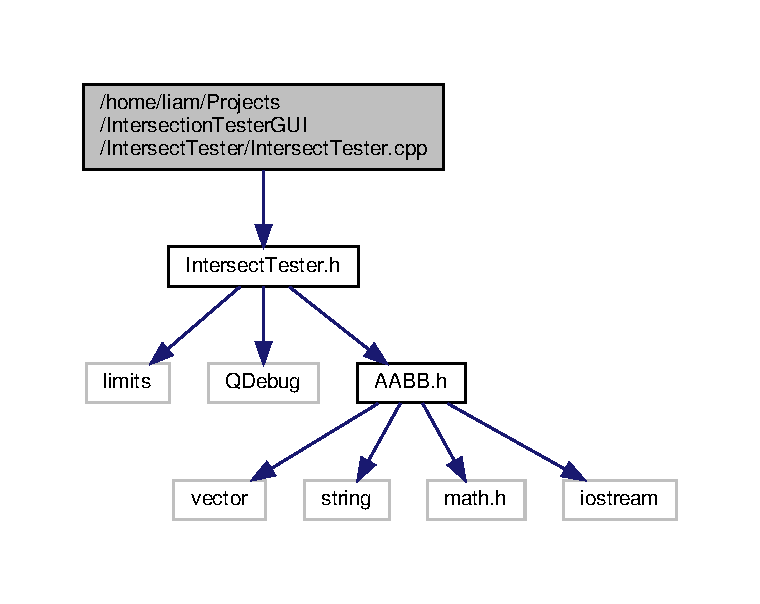
\includegraphics[width=350pt]{_intersect_tester_8cpp__incl}
\end{center}
\end{figure}

\hypertarget{_intersect_tester_8h}{}\section{/home/liam/\+Projects/\+Intersection\+Tester\+G\+U\+I/\+Intersect\+Tester/\+Intersect\+Tester.h File Reference}
\label{_intersect_tester_8h}\index{/home/liam/\+Projects/\+Intersection\+Tester\+G\+U\+I/\+Intersect\+Tester/\+Intersect\+Tester.\+h@{/home/liam/\+Projects/\+Intersection\+Tester\+G\+U\+I/\+Intersect\+Tester/\+Intersect\+Tester.\+h}}
{\ttfamily \#include $<$limits$>$}\newline
{\ttfamily \#include $<$Q\+Debug$>$}\newline
{\ttfamily \#include \char`\"{}A\+A\+B\+B.\+h\char`\"{}}\newline
Include dependency graph for Intersect\+Tester.\+h\+:
\nopagebreak
\begin{figure}[H]
\begin{center}
\leavevmode
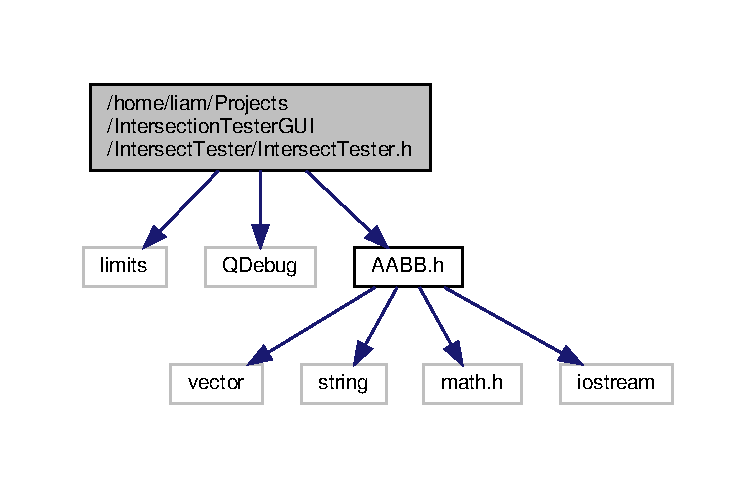
\includegraphics[width=350pt]{_intersect_tester_8h__incl}
\end{center}
\end{figure}
This graph shows which files directly or indirectly include this file\+:
\nopagebreak
\begin{figure}[H]
\begin{center}
\leavevmode
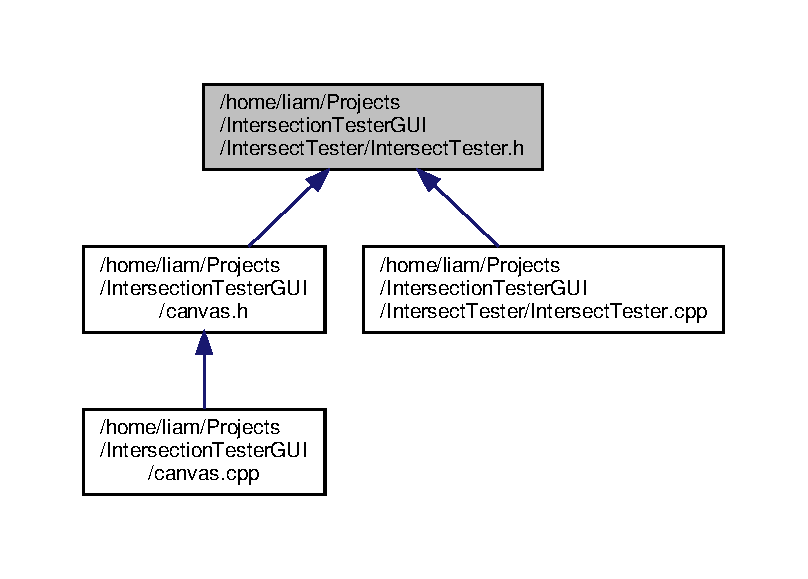
\includegraphics[width=350pt]{_intersect_tester_8h__dep__incl}
\end{center}
\end{figure}
\subsection*{Classes}
\begin{DoxyCompactItemize}
\item 
class \hyperlink{class_point}{Point}
\item 
class \hyperlink{class_line_segment}{Line\+Segment}
\item 
class \hyperlink{class_triangle}{Triangle}
\item 
class \hyperlink{class_circle}{Circle}
\item 
class \hyperlink{class_intersect_tester}{Intersect\+Tester}
\end{DoxyCompactItemize}

\hypertarget{main_8cpp}{}\section{/home/liam/\+Projects/\+Intersection\+Tester\+G\+U\+I/main.cpp File Reference}
\label{main_8cpp}\index{/home/liam/\+Projects/\+Intersection\+Tester\+G\+U\+I/main.\+cpp@{/home/liam/\+Projects/\+Intersection\+Tester\+G\+U\+I/main.\+cpp}}
{\ttfamily \#include \char`\"{}maininterfacewindow.\+h\char`\"{}}\newline
{\ttfamily \#include $<$Q\+Application$>$}\newline
Include dependency graph for main.\+cpp\+:
\nopagebreak
\begin{figure}[H]
\begin{center}
\leavevmode
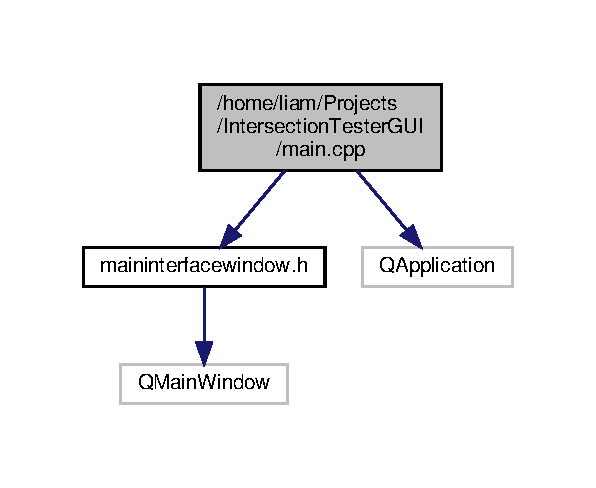
\includegraphics[width=286pt]{main_8cpp__incl}
\end{center}
\end{figure}
\subsection*{Functions}
\begin{DoxyCompactItemize}
\item 
int \hyperlink{main_8cpp_a0ddf1224851353fc92bfbff6f499fa97}{main} (int argc, char $\ast$argv\mbox{[}$\,$\mbox{]})
\end{DoxyCompactItemize}


\subsection{Function Documentation}
\mbox{\Hypertarget{main_8cpp_a0ddf1224851353fc92bfbff6f499fa97}\label{main_8cpp_a0ddf1224851353fc92bfbff6f499fa97}} 
\index{main.\+cpp@{main.\+cpp}!main@{main}}
\index{main@{main}!main.\+cpp@{main.\+cpp}}
\subsubsection{\texorpdfstring{main()}{main()}}
{\footnotesize\ttfamily int main (\begin{DoxyParamCaption}\item[{int}]{argc,  }\item[{char $\ast$}]{argv\mbox{[}$\,$\mbox{]} }\end{DoxyParamCaption})}



Definition at line 4 of file main.\+cpp.


\begin{DoxyCode}
5 \{
6     QApplication a(argc, argv);
7     \hyperlink{class_main_interface_window}{MainInterfaceWindow} w;
8     w.show();
9 
10     \textcolor{keywordflow}{return} a.exec();
11 \}
\end{DoxyCode}

\hypertarget{maininterfacewindow_8cpp}{}\section{/home/liam/\+Projects/\+Intersection\+Tester\+G\+U\+I/maininterfacewindow.cpp File Reference}
\label{maininterfacewindow_8cpp}\index{/home/liam/\+Projects/\+Intersection\+Tester\+G\+U\+I/maininterfacewindow.\+cpp@{/home/liam/\+Projects/\+Intersection\+Tester\+G\+U\+I/maininterfacewindow.\+cpp}}
{\ttfamily \#include \char`\"{}maininterfacewindow.\+h\char`\"{}}\newline
{\ttfamily \#include \char`\"{}ui\+\_\+maininterfacewindow.\+h\char`\"{}}\newline
Include dependency graph for maininterfacewindow.\+cpp\+:
\nopagebreak
\begin{figure}[H]
\begin{center}
\leavevmode
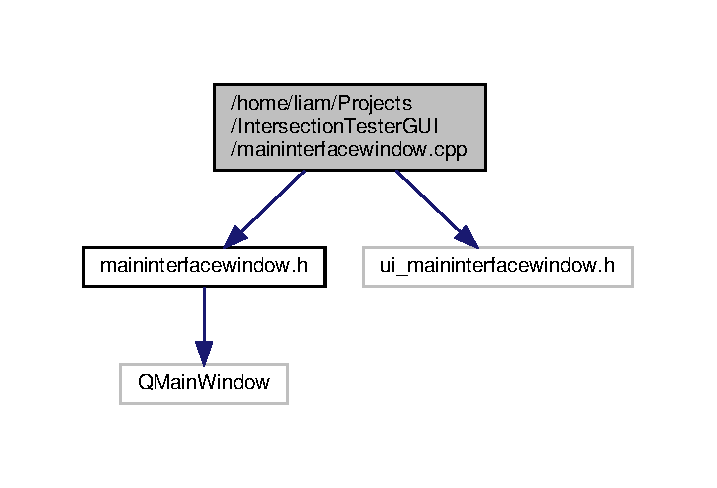
\includegraphics[width=344pt]{maininterfacewindow_8cpp__incl}
\end{center}
\end{figure}

\hypertarget{maininterfacewindow_8h}{}\section{/home/liam/\+Projects/\+Intersection\+Tester\+G\+U\+I/maininterfacewindow.h File Reference}
\label{maininterfacewindow_8h}\index{/home/liam/\+Projects/\+Intersection\+Tester\+G\+U\+I/maininterfacewindow.\+h@{/home/liam/\+Projects/\+Intersection\+Tester\+G\+U\+I/maininterfacewindow.\+h}}
{\ttfamily \#include $<$Q\+Main\+Window$>$}\newline
Include dependency graph for maininterfacewindow.\+h\+:
\nopagebreak
\begin{figure}[H]
\begin{center}
\leavevmode
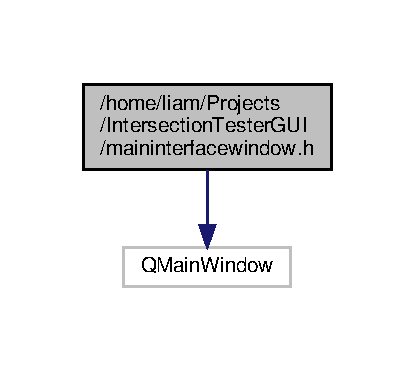
\includegraphics[width=199pt]{maininterfacewindow_8h__incl}
\end{center}
\end{figure}
This graph shows which files directly or indirectly include this file\+:
\nopagebreak
\begin{figure}[H]
\begin{center}
\leavevmode
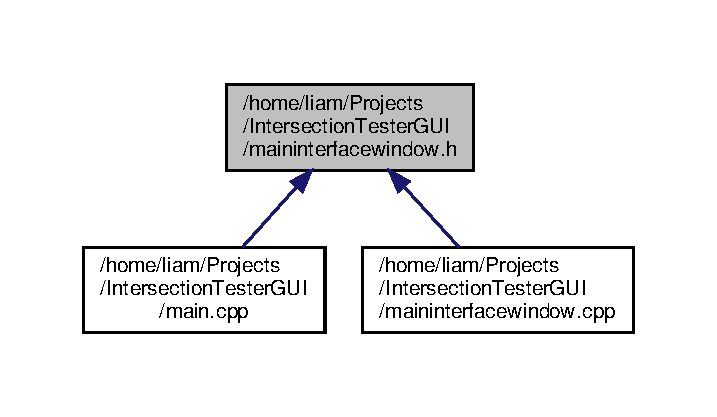
\includegraphics[width=344pt]{maininterfacewindow_8h__dep__incl}
\end{center}
\end{figure}
\subsection*{Classes}
\begin{DoxyCompactItemize}
\item 
class \hyperlink{class_main_interface_window}{Main\+Interface\+Window}
\end{DoxyCompactItemize}
\subsection*{Namespaces}
\begin{DoxyCompactItemize}
\item 
 \hyperlink{namespace_ui}{Ui}
\end{DoxyCompactItemize}

\hypertarget{_r_e_a_d_m_e_8md}{}\section{/home/liam/\+Projects/\+Intersection\+Tester\+G\+U\+I/\+R\+E\+A\+D\+ME.md File Reference}
\label{_r_e_a_d_m_e_8md}\index{/home/liam/\+Projects/\+Intersection\+Tester\+G\+U\+I/\+R\+E\+A\+D\+M\+E.\+md@{/home/liam/\+Projects/\+Intersection\+Tester\+G\+U\+I/\+R\+E\+A\+D\+M\+E.\+md}}

%--- End generated contents ---

% Index
\backmatter
\newpage
\phantomsection
\clearemptydoublepage
\addcontentsline{toc}{chapter}{Index}
\printindex

\end{document}
